%---------------------------------------------------------------------------%
%-                                                                         -%
%-                        Combined Thesis Document                        -%
%-                                                                         -%
%---------------------------------------------------------------------------%
\documentclass[twoside]{Style/ucasthesis}%

%---------------------------------------------------------------------------%
%-                        Helper macros for Combined version (no figures)     -%
%---------------------------------------------------------------------------%
\usepackage{tikz}
\usetikzlibrary{arrows.meta}
\makeatletter
\let\Combined@origincludegraphics\includegraphics
\renewcommand{\includegraphics}[2][]{\Combined@origincludegraphics[#1]{Img/c06h06.png}}
\makeatother

%---------------------------------------------------------------------------%
%-\textrm{e Document settings
%---------------------------------------------------------------------------%
%-\e Document settings
%---------------------------------------------------------------------------%
%---------------------------------------------------------------------------%
%-                        Helper macros for Combined version (no figures)     -%
%---------------------------------------------------------------------------%
%---------------------------------------------------------------------------%
%-\ndocumentclass Document settings
%---------------------------------------------------------------------------%
%-                        Helper macros for Combined version (no figures)     -%
%---------------------------------------------------------------------------%
%---------------------------------------------------------------------------%
%-\e Document settings
%---------------------------------------------------------------------------%
%---------------------------------------------------------------------------%
%->> Document settings
%---------------------------------------------------------------------------%
\usepackage{caption}
\usepackage[super,numbers, list,table,math,tikz]{Style/artratex}
\renewcommand{\topfraction}{0.9}
\renewcommand{\bottomfraction}{0.8}
\renewcommand{\textfraction}{0.07}
\renewcommand{\floatpagefraction}{0.8}
\setlength{\textfloatsep}{10pt plus 2pt minus 2pt}
\usepackage{etoolbox}

%---------------------------------------------------------------------------%
%->> Titlepage information (metadata only, suppress actual generation)
%---------------------------------------------------------------------------%
%---------------------------------------------------------------------------%
%->> Titlepage information
%---------------------------------------------------------------------------%
%-
%-> 中文封面信息
%-
\confidential{}% 密级：涉密论文或延迟公开论文填写
\schoollogo[scale=0.095]{ucas_logo}% 校徽
\title{基于 FPGA 的 SLAM 后端软硬协同加速器设计与实现}% 论文中文题目
\author{张三}% 论文作者
\advisor{我的名字~教授~中国科学院计算机网络信息中心\\}% 指导教师：姓名 专业技术职务 工作单位
%\advisor{指导教师一\\指导教师二\\指导教师三}% 多行指导教师示例
\degree{硕士}% 学位：学士、硕士、博士
\degreetype{工学}% 学位类别：理学、工学、工程、医学等
\major{电子信息}% 一级/二级学科专业名称，领域名称需要与学籍信息一致
\institute{中国科学院大学}% 院系名称
%\institute{中国科学院力学研究所\\流固耦合实验室}% 多行院系名称示例
\date{2026~年~6~月}% 毕业日期：夏季为6月、冬季为12月
%-
%-> 英文封面信息
%-
\TITLE{Design and Implementation of Hardware-Software Co-designed SLAM Backend Accelerator based on FPGA}% 论文英文题目
\AUTHOR{Zhang San}% 论文作者
\ADVISOR{Supervisor: Professor MY NAME}% 指导教师
\DEGREE{Master}% 学位：Bachelor, Master, Doctor, Postdoctor。封面据英文学位名称自动切换，需确保拼写准确
\DEGREETYPE{Engineering}% 学位类别：Philosophy, Natural Science, Engineering, Economics, Agriculture 等
\MAJOR{Electronic Information}% 二级学科专业名称
\INSTITUTE{University of Chinese Academy of Sciences}% 院系名称
\DATE{June, 2026}% 毕业日期：夏季为June、冬季为December
%---------------------------------------------------------------------------%
%
\makeatletter
\@ifundefined{maketitle}{}{%
    \let\Combined@maketitle\maketitle
    \renewcommand{\maketitle}{\relax}%
}
\@ifundefined{MAKETITLE}{}{%
    \let\Combined@MAKETITLE\MAKETITLE
    \renewcommand{\MAKETITLE}{\relax}%
}
\@ifundefined{makedeclaration}{}{%
    \let\Combined@makedeclaration\makedeclaration
    \renewcommand{\makedeclaration}{\relax}%
}
\makeatother

%---------------------------------------------------------------------------%
%->> Document content
%---------------------------------------------------------------------------%
\begin{document}
\mainmatter
\chapter{}
\chapter{}
\chapter{摘要与正文}

\section{中文摘要}
%---------------------------------------------------------------------------%
%-> Chinese abstract content for CombinedThesis
%---------------------------------------------------------------------------%
同步定位与地图构建（Simultaneous Localization and Mapping, SLAM）是自主移动机器人、无人机及增强现实设备实现环境感知与自主导航的核心技术。视觉 SLAM 后端优化涉及大规模稀疏矩阵构建与线性方程组求解，具有极高的计算复杂度与内存访问压力，传统嵌入式 ARM 处理器难以实时完成。针对这一核心矛盾，本文提出并系统实现了一套基于 FPGA 的软硬协同 SLAM 后端加速方案，将"舒尔消元 + EKF 增量更新"的算法策略映射为可在 Zynq UltraScale+ 平台高效运行的异构硬件架构。

在算法层面，本文以 SchurVINS 框架为基础，利用光束法平差（BA）中 Hessian 矩阵的箭形块稀疏结构，通过舒尔补消元将路标点状态从系统中消去，再以单次 EKF 观测更新替代传统 Levenberg--Marquardt 多轮迭代求解，将后端计算主体归结为雅可比累加与 $3 \times 3$ 矩阵求逆两个规则化计算核，实现了算法复杂度与硬件友好性的统一。

在硬件设计层面，本文完成了三项核心工作：（1）设计了 5 级深度流水线雅可比计算模块，覆盖从世界坐标变换、重投影残差计算到 Hessian 矩阵在线累加的完整链路，并通过切换外参常量实现左右目双相机的单硬件路径复用；（2）提出了基于 8 位稀疏观测位图（SOB）编码的两级动态门控机制，在流水线前端实现状态级旁路与相机级时钟门控，自动跳过零块计算，在典型稀疏率 50\% 场景下将总浮点运算量降低约 45\%；（3）实现了针对 $3 \times 3$ 对称矩阵的并行化 Schur 消元核心，以代数余子式法并行计算逆矩阵并利用对称性将输出写操作减少约 50\%，Hessian 矩阵片上 BRAM 占用仅为 67~KB。

在系统架构层面，本文遵循逻辑密集型任务归 PS、数据密集型规则计算归 PL 的原则，在 PS 端 ARM 处理器上运行 SVO 2.0 视觉前端追踪、滑动窗口状态管理与 EKF 位姿更新，将雅可比生成、Hessian 累加与 Schur 消元完全卸载至 PL 端 FPGA 流水线。三通道 AXI 通信架构与双缓冲乒乓调度策略有效隐藏了片外存储访问延迟。

实验结果表明，在 Zynq UltraScale+ ZCU102 平台上，Schur Kernel 将单次后端优化延迟从 2.84~ms 压缩至 0.76~ms，实现 3.74 倍加速比，系统后端优化频率稳定在 25~Hz 以上。在轨迹精度方面，EuRoC 数据集上 FPGA 方案平均绝对轨迹误差（ATE）为 0.073~m，与全软件基准的 0.075~m 精度等价；TUM-VI 数据集上 FPGA 方案平均 ATE 为 0.152~m，优于软件基准的 0.182~m。在能效方面，单帧能耗仅为 19.1~mJ，BRAM 占用为 67~KB，均为同类方案中最优。户外真实场景的部署测试进一步验证了系统的工程可行性。

\keywords{视觉 SLAM，视觉惯性里程计，FPGA，硬件加速，软硬协同，舒尔补消元，稀疏观测位图}


\section{英文摘要}
%---------------------------------------------------------------------------%
%- English abstract content for CombinedThesis
%---------------------------------------------------------------------------%
Simultaneous Localization and Mapping (SLAM) is a fundamental technology enabling environment perception and autonomous navigation for mobile robots, Unmanned Aerial Vehicles (UAVs), and Augmented Reality devices. The backend optimization of visual SLAM involves large-scale sparse matrix construction and linear system solving, imposing prohibitive computational complexity and memory access pressure that conventional embedded ARM processors cannot sustain in real time. To address this critical challenge, this thesis proposes and systematically implements a hardware-software co-designed SLAM backend acceleration scheme based on FPGA, mapping the ``Schur complement elimination + EKF incremental update'' algorithmic strategy onto a heterogeneous hardware architecture running efficiently on the Zynq UltraScale+ platform.

At the algorithmic level, building upon the SchurVINS framework, this work exploits the arrowhead block-sparse structure of the Hessian matrix in Bundle Adjustment (BA), employing Schur complement elimination to marginalize landmark states from the system. A single EKF observation update then replaces the traditional multi-iteration Levenberg--Marquardt solver, reducing the backend computation to two regularized kernels: Jacobian outer-product accumulation and $3 \times 3$ matrix inversion, achieving a unified balance between algorithmic complexity and hardware friendliness.

At the hardware design level, three core contributions are made: (1) A 5-stage deep-pipelined Jacobian computation module is designed, covering the complete chain from world coordinate transformation and reprojection residual calculation to online Hessian matrix accumulation, with stereo camera branch reuse achieved through extrinsic parameter switching on a single hardware datapath. (2) A two-level dynamic gating mechanism based on 8-bit Sparse Observation Bitmap (SOB) encoding is proposed, implementing state-level bypass and camera-level clock gating at the pipeline front-end to automatically skip null-block computations, reducing total floating-point operations by approximately 45\% under a typical 50\% sparsity scenario. (3) A parallelized Schur elimination core targeting $3 \times 3$ symmetric matrices is implemented, computing inverse matrices via the cofactor method in parallel and exploiting output symmetry to reduce write operations by approximately 50\%, with the on-chip BRAM footprint for the Hessian matrix compressed to only 67~KB.

At the system architecture level, following the principle of assigning logic-intensive tasks to the PS and data-intensive regular computations to the PL, the ARM processor on the PS side runs the SVO~2.0 visual front-end tracking, sliding window state management, and EKF pose updates, while Jacobian generation, Hessian accumulation, and Schur elimination are fully offloaded to the FPGA pipeline on the PL side. A three-channel AXI communication architecture combined with a double-buffering ping-pong scheduling strategy effectively hides off-chip memory access latency.

Experimental results on the Zynq UltraScale+ ZCU102 platform demonstrate that the Schur Kernel compresses single backend optimization latency from 2.84~ms to 0.76~ms, achieving a 3.74$\times$ speedup with the system backend optimization frequency sustained above 25~Hz. In terms of trajectory accuracy, the FPGA scheme achieves a mean Absolute Trajectory Error (ATE) of 0.073~m on the EuRoC dataset, equivalent to the 0.075~m of the full-software baseline; on the TUM-VI dataset, the FPGA scheme achieves a mean ATE of 0.152~m, outperforming the software baseline of 0.182~m. In terms of energy efficiency, the per-frame energy consumption is only 19.1~mJ and the BRAM footprint is 67~KB, both representing the best among comparable solutions. Outdoor real-world deployment tests further validate the engineering feasibility of the system.

\KEYWORDS{Visual SLAM, Visual-Inertial Odometry, FPGA, Hardware Acceleration, Hardware-Software Co-design, Schur Complement Elimination, Sparse Observation Bitmap}


%---------------------------------------------------------------------------%
%->> Combined main content (chapters downgraded to sections)
%---------------------------------------------------------------------------%
{%% local scope for heading redefinitions
    \let\chapter\section
    \let\section\subsection
    \let\subsection\subsubsection
    \let\subsubsection\paragraph
    %---------------------------------------------------------------------------%
%->> Main content
%---------------------------------------------------------------------------%
\renewcommand{\thefigure}{\thechapter-\arabic{figure}}
\renewcommand{\thetable}{\thechapter-\arabic{table}}
\renewcommand{\theequation}{\thechapter-\arabic{equation}}
\chapter{绪论}\label{chap:introduction}

\section{研究背景与意义}

同步定位与地图构建（Simultaneous Localization and Mapping, SLAM）是移动机器人、无人机以及增强现实/虚拟现实设备实现自主导航与环境感知的关键技术\cite{thrun2005probabilistic}。在未知或弱先验环境中，系统需依靠机载传感器持续估计自身位姿并构建环境地图，从而为路径规划、任务执行和人机交互提供基础支撑。Cadena 等人\cite{cadena2016past}在其里程碑式的综述中系统回顾了 SLAM 研究三十余年的发展历程，将其划分为经典时代（1986--2004）、算法改进时代（2004--2015）与鲁棒感知时代（2015 至今），指出 SLAM 已从单一的概率推断问题演进为融合几何、语义和深度学习的综合性感知框架。随着视觉传感器的成本持续下降、成像质量提升以及嵌入式计算能力增强，视觉 SLAM 逐渐成为主流方案\cite{gao2017vslam14}，并在空间探测、仓储物流、家庭服务与移动终端等场景中得到广泛应用。

从应用场景看，SLAM 已成为多类智能系统的基础能力。在自动驾驶与配送机器人中，SLAM 为车辆提供高精度定位与动态环境建图，支撑路径规划和安全决策；在无人机与室内巡检中，SLAM 使平台在 GPS 不可用的环境中实现稳定导航\cite{forster2014svo}；在 AR/VR 设备与移动终端中，SLAM 支撑实时空间理解与虚实融合，直接决定交互体验\cite{klein2007parallel}；在仓储、安防与服务机器人场景，SLAM 则提供可重复构建的语义地图与任务级定位能力。图~\ref{fig:slam_applications} 展示了 SLAM 技术在不同领域的典型应用场景。

\begin{figure}[htbp]
    \centering
    \begin{subfigure}[b]{0.48\textwidth}
        \centering
        \includegraphics[width=\textwidth]{Img/scene1_auto_drive_car.png}
        \caption{自动驾驶汽车}
        \label{fig:slam_app_auto_drive}
    \end{subfigure}
    \hfill
    \begin{subfigure}[b]{0.48\textwidth}
        \centering
        \includegraphics[width=\textwidth]{Img/scene2_delivery_robot.png}
        \caption{配送机器人}
        \label{fig:slam_app_delivery}
    \end{subfigure}

    \vspace{0.5em}

    \begin{subfigure}[b]{0.48\textwidth}
        \centering
        \includegraphics[width=\textwidth]{Img/scene3_drone.png}
        \caption{无人机室内导航}
        \label{fig:slam_app_drone}
    \end{subfigure}
    \hfill
    \begin{subfigure}[b]{0.48\textwidth}
        \centering
        \includegraphics[width=\textwidth]{Img/scene4_AR_VR.png}
        \caption{增强/虚拟现实设备}
        \label{fig:slam_app_ar_vr}
    \end{subfigure}

    \vspace{0.5em}

    \begin{subfigure}[b]{0.48\textwidth}
        \centering
        \includegraphics[width=\textwidth]{Img/scene5_industrial_mobile_robot.png}
        \caption{仓储搬运机器人}
        \label{fig:slam_app_warehouse}
    \end{subfigure}
    \hfill
    \begin{subfigure}[b]{0.48\textwidth}
        \centering
        \includegraphics[width=\textwidth]{Img/scene6_security_patrol_robot.png}
        \caption{安防巡检机器人}
        \label{fig:slam_app_security}
    \end{subfigure}

    \vspace{0.5em}

    \begin{subfigure}[b]{0.48\textwidth}
        \centering
        \includegraphics[width=\textwidth]{Img/scene7_humanoid_service_robot.png}
        \caption{家庭服务机器人}
        \label{fig:slam_app_service}
    \end{subfigure}
    \hfill
    \begin{subfigure}[b]{0.48\textwidth}
        \centering
        \includegraphics[width=\textwidth]{Img/scene8_lunar_rover.png}
        \caption{空间探测月球车}
        \label{fig:slam_app_space}
    \end{subfigure}

    \bicaption{SLAM 技术的典型应用场景}{Typical application scenarios of SLAM technology}
    \label{fig:slam_applications}
\end{figure}

SLAM 的发展历史可以追溯到 1980 年代末和 1990 年代初的概率机器人学研究。Thrun 等人\cite{thrun2005probabilistic}在其专著《Probabilistic Robotics》中系统阐述了将概率推断方法应用于机器人感知与决策的理论框架，为 SLAM 的数学建模奠定了基础。这一时期的核心贡献在于将地图构建与定位问题统一在一个概率框架下，特别是 Smith 和 Cheeseman~\cite{smith1988estimating} 提出的状态估计理论，以及 Durrant-Whyte~\cite{durrant1987uncertain} 对不确定性建模的深入探讨。随着 Smith 等人~\cite{smith1990estimating} 明确描述了地标位置与机器人位姿之间的统计相关性，SLAM 作为一个独立的科学问题正式确立。Durrant-Whyte 和 Bailey~\cite{durrantwhyte2006slam} 在其经典的双篇综述教程中（Part I 与 Part II\cite{bailey2006simultaneous}），分别对 SLAM 的概率基础与计算方法进行了系统梳理：Part I 阐述了基于 EKF、粒子滤波与信息滤波的递推贝叶斯框架，深入分析了 SLAM 问题的收敛特性与一致性条件；Part II 则讨论了数据关联、闭环检测和多机器人协作等关键工程问题。此后基于扩展卡尔曼滤波（EKF-SLAM）的方法成为早期最为主流的实现方案。这一阶段的关键认识是地标误差与位姿误差存在强相关性，地图无法拆分为独立估计问题，因此必须在联合状态中统一建模。与此同时，EKF-SLAM 的协方差矩阵随地标数量 $N$ 呈 $O(N^2)$ 增长，计算与存储开销随规模迅速上升，直接推动了后续的 FastSLAM 与图优化框架的发展。进入 2000 年代，随着图优化理论与稀疏线性代数领域的成熟，Kaess 等人先后提出了增量式平滑与建图方法 iSAM\cite{kaess2008isam} 和 iSAM2\cite{kaess2011isam2}，开创性地利用贝叶斯树数据结构实现了因子图的增量更新，使得大规模 SLAM 问题的在线求解成为可能。K{\"u}mmerle 等人\cite{kummerle2011g}提出的通用图优化框架 g$^2$o 则为后续众多 SLAM 系统提供了高效的后端优化引擎，支持多种求解器与鲁棒核函数。2010 年代以来，视觉 SLAM 迅速普及，单目、双目与视觉惯性系统相继成熟，ORB-SLAM\cite{mur2015orb}、LSD-SLAM\cite{engel2014lsd}、SVO\cite{forster2014svo}、OKVIS\cite{leutenegger2015keyframe}、VINS-Mono\cite{qin2018vins} 与 ROVIO\cite{bloesch2015robust} 等经典框架推动了系统在实时性、鲁棒性与多传感器融合方面的进步，ORB-SLAM2/3 进一步扩展到双目、RGB-D 与视觉惯性多地图场景\cite{mur2017orb,campos2021orb}。近年来，深度学习与语义感知开始与 SLAM 融合，使得系统在动态场景与弱纹理环境中的表现进一步增强，同时也对后端优化的算力提出了更高要求。

典型视觉 SLAM 体系通常包含传感器数据获取、前端跟踪、后端优化、回环检测与建图更新等模块，其流程如图~\ref{fig:visual_slam_pipeline} 所示。前端负责特征提取与匹配并给出初始位姿估计，后端通过非线性优化进一步消除累积误差，回环检测与建图模块则保证全局一致性与地图质量。由于视觉测量噪声、光照变化与动态遮挡等因素的存在，前端估计易产生漂移，因此位姿优化成为决定定位精度与系统稳定性的核心环节。

\begin{figure}[htbp]
    \centering
    \resizebox{0.92\linewidth}{!}{\begin{tikzpicture}[node distance=14mm,>=Stealth,rounded corners,thick]
    \tikzstyle{block}=[draw,minimum width=22mm,minimum height=8mm,align=center]
    \tikzstyle{data}=[draw,minimum width=18mm,minimum height=8mm,align=center]

    \node[block] (sensor) {传感器\\数据获取};
    \node[block, right=of sensor] (frontend) {前端\\跟踪与匹配};
    \node[block, right=of frontend] (backend) {后端\\位姿优化};
    \node[block, right=of backend] (loop) {回环\\检测};
    \node[block, below=of backend] (mapping) {建图\\与更新};

    \draw[->] (sensor) -- (frontend);
    \draw[->] (frontend) -- (backend);
    \draw[->] (backend) -- (mapping);
    \draw[->] (loop) -- (backend);
    \draw[->] (backend) -- (loop);
    \draw[->] (mapping) -| (frontend);
\end{tikzpicture}
}
    \bicaption{经典视觉 SLAM 系统流程}{Classic visual SLAM pipeline}
    \label{fig:visual_slam_pipeline}
\end{figure}

在视觉 SLAM 的演进历程中，后端状态估计主要形成了以扩展卡尔曼滤波（EKF）为代表的滤波法和以束调整（Bundle Adjustment, BA）为代表的非线性优化法两大路径。早期的后端方案多采用基于马尔科夫假设的滤波框架，如经典 EKF-SLAM\cite{smith1990estimating}，其核心在于通过预测与更新步骤实时维护状态向量及其协方差矩阵；随后，Mourikis 等人提出的多状态约束卡尔曼滤波（MSCKF）\cite{mourikis2007multi}进一步提升了视觉惯性系统的实时性。滤波法的优势在于计算资源消耗相对可控，通过边际化历史状态实现了极高的处理频率；然而，其固有的线性化误差往往导致系统估计的不一致性，且在处理大规模闭环或长距离漂移时，缺乏重新线性化的机制，容易陷入局部最优。相比之下，基于图优化的非线性优化法\cite{kummerle2011g}逐渐成为当前主流趋势，该方法将定位与建图转化为超定方程的最小二乘问题，通过高斯—牛顿或列文伯格—马夸尔特等算法迭代求解\cite{triggs1999bundle}。优化法的核心优势在于允许对历史状态进行重新线性化，配合滑动窗口或关键帧机制\cite{leutenegger2015keyframe}，能显著提升全局定位精度；然而，这种精度增益是以巨大的计算开销为代价的，优化过程涉及复杂的雅可比矩阵计算、大规模海森矩阵累积以及稀疏线性方程组求解，尽管稀疏性可利用舒尔补进行加速，但随着路标点与关键帧规模的迅速扩张，计算复杂度仍呈指数级增长，形成显著的后端性能瓶颈。在高频视觉输入与实时性需求下，这种计算密集的特性使得后端优化在移动端和嵌入式平台上难以满足低延时要求。传统的通用处理器（CPU）或图形处理器（GPU）虽然具备极高的编程灵活性，但受限于功耗与能效比，难以在小型无人机、可穿戴 AR 设备等对功耗极度敏感的场景中长期稳定运行。因此，针对后端优化算法中矩阵运算的底层特征进行硬件架构级的加速设计，已成为突破 SLAM 系统实时性瓶颈的关键方向。

与通用处理器相比，现场可编程门阵列（Field-Programmable Gate Array, FPGA）具备高度并行、确定性时延与可定制存储层级的优势，能够以更低能耗实现稀疏矩阵运算、雅可比流水线与舒尔补求解等核心算子，从而为 SLAM 后端优化提供更高的实时性保障\cite{huangkun2025vslam}。通过软硬协同的设计方式，将计算密集的位姿优化环节迁移至 FPGA，同时在处理器端保留系统控制与轻量更新逻辑，可在保持精度的同时显著降低延时与功耗。这不仅有助于推动视觉 SLAM 在资源受限平台上的落地，也为高可靠、自主运行的智能系统提供关键支撑。

\section{国内外研究现状}

针对视觉 SLAM 及其后端优化的加速研究，国内外学者从算法改进与硬件架构设计两个维度开展了大量工作。本节将从软件算法演进、国外研究现状以及国内研究进展三个方面进行综述。

\subsection{系统框架与软件算法演进}

视觉 SLAM 算法的演进是一个多种理论不断交叉融合的过程，从早期的滤波机制到现代的非线性优化，再到如今引入深度学习模型，其系统框架在精度、鲁棒性以及计算复杂度上不断寻求平衡。本节将从前端数据关联方式、后端状态估计框架以及深度学习的融合三个维度，对视觉 SLAM 的软件算法演进进行阐述。

\subsubsection{视觉前端数据关联}

视觉前端的主要任务是从图像流中提取特征并建立帧间数据关联，进而为后端提供初始的相机运动估计。根据数据关联方式的不同，前端主要分为间接法、直接法和半直接法三大类。

间接法（特征点法）是目前最为成熟和广泛应用的前端方案。该方法首先从图像中提取具有代表性的关键点并计算相应的描述子，随后通过描述子匹配建立相邻帧之间的 2D-2D 或 2D-3D 数据关联，最后通过最小化重投影误差（Reprojection Error）求解相机位姿。在特征提取器的发展历程中，Lowe\cite{lowe2004distinctive} 于 2004 年提出的尺度不变特征变换（SIFT）是里程碑式的工作，该算法通过构建高斯差分尺度空间检测关键点，并以关键点邻域梯度直方图作为 128 维描述子，具有良好的旋转、尺度与仿射不变性，但其计算开销较大（单帧需数百毫秒），难以满足实时性要求。Bay 等人\cite{bay2008surf} 提出的加速稳健特征（SURF）利用积分图像与 Haar 小波近似替代 SIFT 中的高斯卷积，将计算速度提升约 3 倍，但仍无法满足嵌入式平台的帧率需求。为此，Rublee 等人\cite{rublee2011orb} 在 2011 年提出了 ORB（Oriented FAST and Rotated BRIEF）描述子，结合 Rosten 和 Drummond\cite{rosten2006machine} 设计的高速 FAST 角点检测器与旋转 BRIEF 二进制描述子，在保持良好匹配性能的同时将单帧计算压缩到毫秒级别，成为当前实时 SLAM 系统中应用最为广泛的手工特征。间接法的优势在于对光照变化和图像模糊具有较强的鲁棒性，且提取的几何特征便于后端进行优化与回环检测。

在系统层面，Klein 和 Murray\cite{klein2007parallel} 于 2007 年提出的 PTAM（Parallel Tracking and Mapping）开创性地将跟踪与建图分离到两个并行线程，首次在增强现实场景中实现了实时的关键帧式 BA 优化，标志着 SLAM 从滤波范式向优化范式的重要转折。此后，Mur-Artal 等人\cite{mur2015orb}提出的 ORB-SLAM 将 ORB 特征、共视图（Covisibility Graph）与 G{\'a}lvez-L{\'o}pez 和 Tard{\'o}s\cite{galvez2012bags} 提出的词袋（Bag of Binary Words, DBoW2）回环检测融为一体，构建了包含跟踪、局部建图与闭环三线程的完整系统架构。ORB-SLAM2\cite{mur2017orb} 将支持范围从单目扩展到双目与 RGB-D 相机，ORB-SLAM3\cite{campos2021orb} 进一步集成了视觉惯性紧耦合与多地图管理能力，成为当前功能最完备的开源特征点法 SLAM 系统。然而，特征提取和匹配过程极为耗时，往往构成了前端计算资源的瓶颈，尤其在高分辨率图像或高帧率场景下，ORB 提取可占据前端超过 60\% 的计算时间。

直接法（Direct Method）的提出旨在跳过耗时的特征提取环节。它基于灰度不变性假设（即空间中同一点在不同视角下的像素灰度保持不变），通过直接最小化光度误差（Photometric Error）来估计相机运动。直接法能够利用图像中的像素点（包括边缘和无明显角点区域），在弱纹理环境中表现出更好的鲁棒性。Newcombe 等人\cite{newcombe2011dtam}提出的 DTAM（Dense Tracking and Mapping）是最早的实时稠密直接法系统之一，通过最小化全图光度误差同时恢复相机运动与稠密深度图，但依赖 GPU 并行计算。Engel 等人\cite{engel2014lsd}提出的 LSD-SLAM（Large-Scale Direct Monocular SLAM）将直接法与半稠密重建结合，在单目 CPU 上实现了大规模环境的实时建图。此后，Engel 等人\cite{engel2017direct}进一步提出了 DSO（Direct Sparse Odometry），放弃了 LSD-SLAM 中的稠密重建策略，改为在图像中选取具有强梯度的稀疏像素点进行联合光度优化，同时显式建模几何参数（逆深度）与光度参数（曝光时间与暗角），在保持直接法灵活性的同时显著提升了精度与效率。尽管直接法省去了特征计算，但由于局部光度梯度的非凸性，其对相机的剧烈运动和光照突变极为敏感，容易陷入局部最优。

为了结合上述两者的优势，半直接法（Semi-direct Method）应运而生。半直接法通常仅提取 FAST 角点但不计算描述子，利用光流法或直接法追踪这些特征点，随后再结合特征对齐提升定位精度。它在一定程度上避免了直接法的非凸性问题，同时免去了特征点法冗长的描述子匹配开销。Forster 等人\cite{forster2014svo}于 2014 年提出的 SVO（Semi-direct Visual Odometry）是该领域的标杆算法，其将稀疏图像对齐（Sparse Image Alignment）与特征对齐（Feature Alignment）级联，凭借极高的前端运行帧率（在标准测试中可达 300~fps 以上）和良好的精度，成为微型飞行器（MAV）等计算受限平台的理想框架。SVO 2.0\cite{forster2017svo} 进一步扩展了多相机支持与边缘特征利用，显著提升了系统在宽基线与大视场角场景下的鲁棒性。

\subsubsection{后端状态估计框架}

视觉 SLAM 的后端负责消除前端的累积漂移，通过融合多源测量（如 IMU、里程计等）维持全局一致的地图。按照状态估计类型的不同，主要分为滤波法和优化法两大路径。

滤波法（Filter-based）主要基于马尔科夫假设，利用贝叶斯滤波框架在当前时刻更新系统状态与协方差矩阵。早期的单目 MonoSLAM\cite{davison2007monoslam} 采用了扩展卡尔曼滤波（EKF）框架，将相机位姿与路标点共同纳入状态向量进行更新。Davison 等人的贡献在于首次证明了单目相机在未知环境中能够实时完成概率性的自主建图，但由于状态向量和协方差矩阵的大小随路标点的增加而膨胀，其计算量呈平方级增长（$O(N^2)$），严重限制了地图的大规模扩展。为解决此问题，Mourikis 和 Roumeliotis\cite{mourikis2007multi} 提出了 MSCKF（Multi-State Constraint Kalman Filter），其核心思想是在状态向量中仅维护滑动窗口内的历史位姿，将针对同一路标的多帧观测投影到零空间消除路标状态，使计算复杂度仅与窗口大小相关而非路标数量。MSCKF 极大地提升了系统的实时性，成为了视觉惯性里程计（VIO）领域的经典方案，并广泛应用于 Google ARCore 等工业级产品。Geneva 等人\cite{geneva2020openvins}在 ICRA 2020 上发布的 OpenVINS 开源平台系统整合了 MSCKF 的多种变体与扩展（包括 SLAM 特征、FEJ 一致性保证、在线标定等），为 VIO 算法的研究与对比评估提供了统一基准。Bloesch 等人\cite{bloesch2015robust}提出的 ROVIO（Robust Visual Inertial Odometry）则将直接法光度误差引入 EKF 更新步骤，避免了特征提取与匹配的开销，在计算资源极为有限的场景下展现出良好的实时性。

随着图优化理论与稀疏矩阵线性代数求解器领域的成熟，优化法（Optimization-based）逐渐取代滤波法成为主流框架。Kaess 等人\cite{kaess2008isam}于 2008 年提出的 iSAM（Incremental Smoothing and Mapping）首次实现了因子图的增量式 QR 分解更新，避免了每次新增观测时对整个信息矩阵的重新分解。此后，iSAM2\cite{kaess2011isam2} 引入贝叶斯树（Bayes Tree）数据结构，实现了增量式变量重排序与流体式重新线性化（Fluid Relinearization），使得仅受新观测影响的局部子图被更新，极大提升了大规模地图的在线求解效率。K{\"u}mmerle 等人\cite{kummerle2011g}提出的通用图优化框架 g$^2$o（General Graph Optimization）为后续众多 SLAM 系统提供了高效的后端优化引擎，其采用稀疏 Cholesky 分解求解正规方程，支持多种鲁棒核函数与求解策略，已被 ORB-SLAM、LSD-SLAM 等系统广泛采用。优化法将所有或一段滑动窗口内的历史轨迹及路标点构建为一个超大的非线性最小二乘图，通过束调整（Bundle Adjustment, BA）全局解算位姿与路标。Triggs 等人\cite{triggs1999bundle}在其经典的综述中系统总结了 BA 的理论基础与实现方法，指出 BA 本质上是一个在流形上的稀疏非线性最小二乘问题，其海森矩阵（Hessian Matrix）天然具有箭头形稀疏结构，可通过舒尔补（Schur Complement）消元将路标变量边际化，从而将求解规模从 $(N_p + N_m)$ 降至 $N_p$（$N_p$ 为位姿数，$N_m$ 为路标数），这一思想构成了本文硬件加速器设计的算法基础。

在视觉惯性融合方面，IMU 预积分理论的提出是重要的里程碑。Lupton 和 Sukkarieh\cite{lupton2012visual} 于 2012 年首次提出了 IMU 预积分（Preintegration）的概念，将相邻关键帧之间的高频 IMU 测量预先积分为相对运动约束，避免了偏置更新时对所有 IMU 数据的重新积分。Forster 等人\cite{forster2017onmanifold}在此基础上进一步发展了流形上的预积分理论（On-Manifold Preintegration），通过在 $SO(3)$ 流形上直接进行旋转积分，消除了欧拉角或四元数参数化带来的奇异性问题，并推导了协方差传播与偏置修正的解析公式，成为当前 VIO 系统（如 VINS-Mono、OKVIS、ORB-SLAM3）普遍采用的标准方法。

当前主流系统如 ORB-SLAM 系列、OKVIS\cite{leutenegger2015keyframe} 以及 VINS-Mono\cite{qin2018vins} 均采用优化法。其中，Leutenegger 等人\cite{leutenegger2015keyframe}提出的 OKVIS 是最早的基于关键帧的视觉惯性非线性优化系统之一，通过在滑动窗口中联合优化相机位姿、速度、IMU 偏置与路标点，建立了紧耦合 VIO 的基本范式。Qin 等人\cite{qin2018vins}提出的 VINS-Mono 进一步将滑动窗口机制与预积分技术相结合，创新性地设计了边缘化（Marginalization）策略将早期状态信息转化为先验融入系统，并引入了在线时序标定\cite{qin2018online}以处理视觉与惯性传感器之间的时间偏移，在 EuRoC\cite{Burri25012016} 等权威数据集上展现了优异的精度表现。此外，Fan 等人\cite{fan2024schurvins}在 CVPR 2024 上提出的 SchurVINS 通过将舒尔补消元与误差状态卡尔曼滤波（EKF）增量更新相结合，以极低的计算代价实现了接近全 BA 优化的精度，为嵌入式平台上的 VIO 部署提供了轻量化解决方案，本文的硬件加速架构正是基于该算法框架展开设计的。

\subsubsection{深度学习与视觉 SLAM 的融合}

近年来，深度学习技术正在逐步渗透到 SLAM 的各个模块中，从特征提取与匹配到深度估计与端到端位姿回归，深层神经网络通过数据驱动的方式展现出了应对复杂动态场景、弱纹理区域以及剧烈光照变化的强大能力。

在前端特征提取层面，DeTone 等人\cite{detone2018superpoint}于 2018 年提出的 SuperPoint 网络采用自监督训练策略，通过单应性变换（Homographic Adaptation）从合成几何图形迁移学习到真实图像，能够在单次前向推理中同时输出关键点位置及其 256 维描述子。相比传统的 FAST/ORB 提取器，SuperPoint 在光照变化、视角变换与运动模糊条件下展现出显著更强的重复性与匹配稳定性。在此基础上，Sarlin 等人\cite{sarlin2020superglue}于 CVPR 2020 提出的 SuperGlue 利用图神经网络（Graph Neural Network）与注意力机制对关键点集合进行联合推理，通过可微分的 Sinkhorn 最优传输算法建立跨图像的特征对应关系，显著提升了宽基线、重复纹理和弱纹理场景下的匹配精度。Sun 等人\cite{sun2021loftr}在 CVPR 2021 进一步提出了 LoFTR（Local Feature Matching with Transformers），该方法完全摒弃了关键点检测步骤，利用 Transformer 的全局感受野在粗粒度特征图上建立稠密对应，再通过精细化模块提取亚像素级匹配。LoFTR 在室内弱纹理环境（如白墙、走廊）中表现尤为突出，为无纹理区域的视觉定位提供了新的思路。

在深层多视图几何理解方面，Teed 和 Deng\cite{teed2020raft} 提出了基于全对偶场循环架构的 RAFT（Recurrent All-Pairs Field Transforms）用于准确预估光流。RAFT 构建了 4D 全对偶相关体（Correlation Volume），并通过 GRU 循环单元迭代更新光流场，在 Sintel 和 KITTI 基准上取得了突破性的精度提升。到了系统层面，Teed 和 Deng\cite{zhu2020droid} 进一步提出了端到端的 DROID-SLAM，利用循环 GRU 模块迭代更新相机位姿与像素级对应场，在前端跟踪阶段采用稠密 BA 层（Dense BA Layer）通过可微分的 Gauss-Newton 求解实时优化位姿与深度，后端则借助全局 BA 消除累积漂移。DROID-SLAM 在 TartanAir、EuRoC 与 TUM-RGBD 等多种基准上均达到了与经典几何方法可比甚至超越的精度，特别是在大运动与严重模糊条件下展现出了显著优于传统方法的鲁棒性。

尽管深度学习 SLAM 展现出了高鲁棒性与语义感知潜力，但其依赖高性能 GPU 运算的特性（DROID-SLAM 在 NVIDIA RTX 3090 上仍仅能以约 10~fps 运行），极大地限制了其在功耗和算力受限的边缘芯片平台上的大规模部署。此外，深度学习方法对训练数据分布的依赖使其泛化能力仍有待提升。因此，在当前的嵌入式 SLAM 系统中，基于传统几何方法的优化后端仍然是保证实时性与可靠性的主流选择。

\subsubsection{后端优化的计算瓶颈分析}

综上所述，虽然基于优化法（BA）的 SLAM 在精度与鲁棒性方面表现优异，但在嵌入式系统中它却带来了沉重的计算负担。莫霄睿等人\cite{mo2024ba_review}在其综述中系统分析了 BA 优化芯片的研究现状，指出一次典型的后端 BA 优化需要经历雅可比矩阵求导（Jacobian Computation）、海森矩阵累积（Hessian Accumulation）、舒尔补消元（Schur Complement Elimination）以及线性方程组求解（Linear System Solving）等多个计算密集阶段。以滑动窗口大小为 4、路标点数量为 200 的典型 VIO 场景为例，单次优化迭代需要完成约 $4 \times 200 \times 2 = 1600$ 次雅可比计算（考虑双目），累积 $6 \times 6$ 位姿块与 $3 \times 3$ 路标块共计数千个海森子矩阵，并最终求解 24 维的舒尔补正规方程组。Gan 等人\cite{gan2021eudoxus}在 HPCA 2021 上发表的 Eudoxus 工作中，通过对自动驾驶定位系统的系统性性能剖析（Profiling），量化揭示了后端优化在总计算时间中占比高达 70\%--90\% 的事实，其中舒尔补与矩阵求解是最主要的热点函数。这一复杂的矩阵迭代过程在移动终端（如基于 ARM 处理器的无人机或 AR 设备上）产生了几十到上百毫秒量级的延迟，成为制约系统实时性与能效比的瓶颈。

针对 SLAM 的高昂算力需求，学术界首先在前端探索了专用领域的硬件加速方案。Fang 等人\cite{fang2017fpga_orb}早在 2017 年就在 ICFPT 会议上展示了基于 FPGA 的 ORB 特征提取加速器，将 FAST 角点检测与 BRIEF 描述子计算整合到统一流水线中。此后，Liu 等人设计的 eSLAM\cite{liu2019eslam} 在 DAC 2019 上提出了面向完整 ORB-SLAM 前端的节能加速器，通过 FPGA 全流水线成功实现了高速特征检测、描述子计算与帧间匹配的端到端加速，相比 ARM Cortex-A9 实现了 3 倍加速与 61\% 的能耗节省。Fang 等人\cite{fang2019fpga}则在 IEEE TCAS-I 上发表了针对视觉 SLAM 前端的系统化加速架构，将特征提取、光流跟踪与位姿估计集成为统一的硬件流水线。Zhang 等人\cite{zhang2023fpga_feature}在 2023 年进一步提出了同时支持特征提取与追踪的 FPGA 加速器，通过并行化 Lucas-Kanade 光流计算实现了更高的前端吞吐率。然而，当前端的处理能力得到了成倍的提升后，原本就吃紧的后端优化阶段面临着更加密集的特征点输入约束。这意味着必须突破通用处理器的计算瓶颈，针对基于 BA 的稀疏矩阵运算法则设计更深层级与更大规模数据的专用处理架构，方能在低功耗平台满足 SLAM 复杂算法迭代的需要。因此，将目光聚焦于通过软硬协同或者底层算子加速来提升 SLAM 后端运算效率，已成为了突破嵌入式领域自动导航系统性能天花板的必由之路。

\subsection{国外研究现状}

国外顶尖高校与研究机构在 SLAM 硬件加速领域起步较早，研究重点已从早期的前端特征提取加速逐渐转向后端非线性优化与稀疏矩阵求解器的深度定制化设计。根据目标硬件平台的不同，相关工作可分为基于 FPGA 的前端视觉加速器、基于 FPGA 的后端优化加速器、基于 ASIC 的专用芯片流片以及基于 GPU 的并行优化等方向。

\subsubsection{基于 FPGA 的前端视觉加速器}

SLAM 前端的计算负载主要集中在特征提取与匹配、光流跟踪以及立体深度估计等环节。由于这些操作具有高度的数据级并行性与规则的访存模式，非常适合在 FPGA 上以流水线方式实现。

在特征提取加速方面，除前文提及的 Fang 等人\cite{fang2017fpga_orb}的 ORB 加速器和 Liu 等人\cite{liu2019eslam}的 eSLAM 系统外，清华大学电子工程系 Xu 等人\cite{xu2020cnn_fpga}于 FCCM 2020 上提出了基于 CNN 的 FPGA 特征点提取加速器，将轻量级卷积神经网络部署到嵌入式 FPGA 上，替代传统的手工特征（如 ORB/FAST），在保持与 SuperPoint 相当的检测精度的同时，实现了实时推理速度。该工作展示了深度学习特征在嵌入式 FPGA 上的可行性，为 SLAM 前端从手工特征向学习型特征的迁移提供了硬件基础。Han 和 Liu\cite{han2025orb_fpga}在 ICFPT 2025 上进一步提出了采用循环缓冲架构的 ORB 特征提取 FPGA 加速器，专门面向双目视觉 SLAM 场景，通过时间复用策略在单一硬件实例上交替处理左右目图像，有效降低了资源占用。

在角点检测与特征跟踪方面，Gu 等人\cite{gu2022harris}于 IROS 2022 上提出了面向视觉惯性里程计（VIO）的高能效 Harris 角点检测 FPGA 加速器。该工作来自清华大学精密仪器系，将 Harris 角点检测算法的梯度计算、自相关矩阵累积与非极大值抑制三个阶段整合到统一的像素级流水线中，在 Xilinx Zynq FPGA 上实现了实时 VIO 处理。在光流跟踪方面，Jang 等人\cite{jang2009klt}早在 2009 年就在 ITSC 会议上报告了金字塔 KLT（Kanade-Lucas-Tomasi）光流跟踪器的硬件实现，通过层次化的多分辨率光流计算与流水线化的迭代求解，实现了面向驾驶辅助系统的实时特征跟踪，为后续 SLAM 前端的光流硬件加速奠定了基础。Blachut 和 Kryjak\cite{blachut2022lk_fpga}在 2022 年进一步实现了多尺度 Lucas-Kanade 与 Horn-Schunck 光流算法在 FPGA 上的高效部署，通过像素级流水线与多分辨率金字塔并行计算，在 4K 分辨率视频流上实现了实时光流估计。Zhang 等人\cite{zhang2023fpga_feature}在 2023 年则进一步提出了同时支持特征提取与 Lucas-Kanade 光流追踪的 FPGA 加速器，通过并行化光流计算实现了更高的前端吞吐率。

在立体视觉与深度估计方面，双目立体匹配是 SLAM 系统获取稠密深度信息的重要途径。Banz 等人\cite{banz2010sgm}于 2010 年在 SAMOS 会议上首次系统地报告了半全局匹配（Semi-Global Matching, SGM）算法的 FPGA 实时实现方案，通过沿多个方向并行传播代价体（Cost Volume）并设计片上缓存策略来满足 SGM 算法的高带宽需求，实现了实时的稠密视差图计算。Shrivastava 等人\cite{shrivastava2020sgm}在 FPL 2020 上进一步提出了通过松弛 SGM 中路径间数据依赖关系来提升并行度的方法，在不显著降低视差图质量的前提下，将 FPGA 上的立体匹配吞吐率提升了 2 倍以上。

近年来，基于深度学习的光流估计模型（如 RAFT\cite{teed2020raft}）在精度上取得了突破性进展，其 FPGA 加速也成为新的研究热点。中山大学 Ling 等人\cite{ling2022flowacc}于 DATE 2022 上提出了 FlowAcc，这是首个面向基于 DNN 的光流估计的实时 FPGA 加速器，通过模型压缩与定制化数据流设计，在保持与 GPU 实现相当精度的同时实现了低功耗实时推理。同一团队的 Yan 等人\cite{yan2023optflow}在 Journal of Systems Architecture 2023 上发表了该工作的期刊扩展版本，进一步优化了加速器架构与量化策略。西安交通大学的 Jia 等人\cite{jia2025raft_fpga}于 ISCAS 2025 上专门针对 RAFT 的循环全对偶场变换（Recurrent All-Pairs Field Transforms）架构设计了 FPGA 加速器，通过特征相关体（Correlation Volume）的分块计算与 GRU 迭代单元的硬件映射，实现了端到端的实时光流估计。复旦大学的 Li 等人\cite{li2024optflow_slam}在 A-SSCC 2024 上则提出了面向 SLAM 场景的基于光流的 FPGA 加速器，创新性地利用帧间相似性（Inter-Frame Similarity）减少冗余计算，并采用相关性引导的混合精度流更新策略（Correlation-Guided Mixed-Precision Flow Update），在保持定位精度的同时显著降低了计算量与功耗。

上述前端加速工作表明，随着前端处理能力的大幅提升，后端优化环节的计算压力进一步加剧，因此针对后端的专用加速器设计变得尤为迫切。

\subsubsection{基于 FPGA 的后端加速器}

FPGA 凭借其高度可重构性、确定性时延以及相比 ASIC 更短的开发周期，成为 SLAM 后端加速研究的主流平台。早期的探索性工作中，T{\"o}rtei Tertei 等人\cite{tertei2016ekf_fpga}于 2016 年在 Computers \& Electrical Engineering 期刊上报告了面向三维视觉 SLAM 的 EKF 块加速器 FPGA 设计，通过将 EKF 更新步骤中的矩阵运算模块化并映射到 FPGA 流水线，验证了滤波法后端在可编程逻辑上的实现可行性，为后续优化法后端的 FPGA 加速提供了早期参考。

在该方向上，最具影响力的早期工作是 Liu 等人的 $\pi$-BA 系列。Qin 等人\cite{qin2019piba}于 2019 年在 FCCM 会议上首次提出了嵌入式 FPGA SoC 上的 BA 加速引擎 $\pi$-BA，该工作针对 BA 中三维点共观测（Co-observation）分布的不均匀性进行了深入分析，设计了基于共观测优化的计算调度策略，使硬件能够跳过大量无效的零块运算。$\pi$-BA 在 Xilinx ZC706 FPGA 上采用 Levenberg-Marquardt（LM）优化方法进行验证，将 Schur 消元算法部署到可编程逻辑端进行硬件加速，线性方程组求解等步骤则交由处理器系统（PS）端完成，实现了软硬协同的 BA 加速。Liu 等人\cite{liu2020pi}随后在 IEEE Transactions on Computers 上发表了 $\pi$-BA 的期刊扩展版本，进一步深化了共观测分布理论，完善了完整的 PL 端 BA 部署方案——包括利用非线性最小二乘（NLS）求解器计算 Jacobian 矩阵、通过 Schur 消元简化线性系统、以及通过 Cholesky 分解进行最终求解。通过硬件模块实现流水线并行与动态优化控制（动态调节 NLS 迭代次数和 Schur 消元模块数量），该工作在高效利用计算资源与提升系统效率方面取得了显著进展。

上海交通大学的 Sun 等人\cite{sun2020bax}在 2020 年提出了 BA 加速器 BAX，创新性地采用了访存/执行分离（Decoupled Access/Execute）的体系结构来缓解 BA 计算中严重的访存瓶颈。BAX 将内存访问与计算流水线分离到独立数据通路中，通过片内存储访问单元（Memory Access Unit, MAU）预取数据并分层缓存至计算流水线，同时设计了 3 种无转置矩阵乘法的数据流模式以减少矩阵转置操作带来的额外访存开销。在 Xilinx ZCU102 FPGA 上，BAX 在 200~MHz 频率下功耗仅为 1.12~W，相比 Intel i7-8700 桌面 CPU 实现了 1.73 倍的速度提升，相比 ARM Cortex-A53 嵌入式 CPU 则获得了 22.38 倍的加速。

麻省理工学院（MIT）的 Vivienne Sze 团队在低功耗视觉导航芯片设计方面做出了开创性工作。其代表作 Navion~\cite{suleiman2019navion} 是一款集成视觉惯性里程计（VIO）加速的 65~nm 专用 ASIC 芯片，功耗仅 24~mW。该芯片针对非线性优化中的稀疏性进行了深度挖掘，设计了专用的 Gauss-Newton 求解器，并采用二维稀疏块存储结构，相比移动端 CPU 实现了 171 倍的能效提升。此前，Suleiman 等人\cite{suleiman2018navion}在 2018 年 VLSI Circuits Symposium 上报告了 Navion 的初始设计，展示了将完整 VIO 流水线（包括特征跟踪、IMU 积分、非线性优化与更新）集成到单芯片上的可行性。虽然 Navion 针对 ASIC 流片设计，但其稀疏性利用策略与存储优化思想对 FPGA 架构设计极具启发价值。

Gan 等人\cite{gan2021eudoxus}于 HPCA 2021 上发表的 Eudoxus 是对自动驾驶定位系统进行系统性计算特征分析的代表性工作。该工作对包括 ORB-SLAM2、VINS-Mono 在内的多种主流定位算法进行了深入的性能剖析（Profiling），量化揭示了后端优化中矩阵运算（特别是 Hessian 矩阵构建与 Schur 补求解）在总计算时间中占比高达 70\%--90\% 的事实，并据此提出了针对热点函数的专用加速器设计方法学。在此基础上，Liu 等人\cite{liu2021archytas}在 MICRO 2021 上提出了 Archytas 框架，将加速器综合（Accelerator Synthesis）与运行时动态优化相结合，能够根据不同 SLAM 算法的计算特征自动生成定制化的硬件加速器。Archytas 通过参数化的硬件模板库和编译器驱动的设计空间探索，显著降低了 SLAM 加速器的开发成本。Liu 等人\cite{liu2022cicc}在 CICC 2022 上进一步提出了运行时可重构的 FPGA 加速器，支持在不同定位算法之间动态切换，并在 IEEE Transactions on Computers\cite{liu2022reconfig} 上发表了期刊扩展版本。

加州大学伯克利分校（UC Berkeley）的 Sophia Shao 团队在 2025 年 ASPLOS 会议上提出的 SuperNoVA 架构~\cite{zhao2025supernova}代表了算法-硬件协同设计（Algorithm-Hardware Co-Design）的最新趋势。该工作针对 SLAM 后端的计算延迟瓶颈，提出了资源感知的稀疏矩阵计算数据流架构，专门优化了 BA 过程中的舒尔补操作。通过动态调度与流水线重叠技术，SuperNoVA 在 Xilinx ZCU102 平台上实现了 10~ms 级别的后端优化延迟，相比 NVIDIA Jetson TX2 嵌入式 GPU 降低了 3.2 倍延迟并节省了 68\% 的能耗。

伦敦帝国理工学院（Imperial College London）Christos-Savvas Bouganis 团队探索了基于高斯置信度传播（Gaussian Belief Propagation, GBP）的分布式优化架构。传统的 BA 求解器（如 LM 或 Gauss-Newton）采用集中式策略，需要构建并分解全局 Hessian 矩阵，其计算模式天然适合序列化处理但难以充分发挥 FPGA 的并行优势。Sharif 等人在 DATE 2024 会议上提出的 GBP 加速框架~\cite{sharif2024framework}，通过高度并行的消息传递机制替代传统的集中式求解器，将全局 BA 问题分解为局部子问题并行求解。在因子图的每个节点上，GBP 通过迭代传递高斯分布形式的消息来达成全局一致的状态估计。该框架在 Xilinx Zynq-7000 平台上实现了 5.8 倍加速比，展示了非传统优化算法在硬件加速领域的应用潜力。

多伦多大学的 Chen 和 Anderson~\cite{chen2021fpga}则专注于稀疏 Cholesky 分解的硬件加速，这是 BA 求解器中的核心子模块。SLAM 后端优化中的正规方程 $\mathbf{H}\Delta\mathbf{x} = \mathbf{b}$ 通常通过 Cholesky 分解 $\mathbf{H} = \mathbf{L}\mathbf{L}^\mathrm{T}$ 求解。针对 SLAM 优化过程中稀疏模式动态变化的特点（不同时刻的共视关系导致 Hessian 矩阵的稀疏结构不断改变），Chen 等人提出了基于运行时任务调度的自适应求解器架构，通过符号分解预处理与数值分解流水化，在 Intel Arria~10 FPGA 上实现了相比 Intel MKL 库 2.1 倍的加速。该工作为处理不规则稀疏矩阵运算提供了硬件调度层面的解决方案。

此外，香港城市大学 Cheung 团队的郭润洲等人~\cite{guo2022fpga}针对双目视觉里程计的局部 BA 优化，在 Xilinx Zynq UltraScale+ MPSoC 上设计了专用加速器。该工作将矩阵乘加速器与预条件共轭梯度（PCG）求解器相结合，实现了 Jacobian 矩阵生成与 Hessian 矩阵累积的流水线并行，相比 Intel x86 处理器实现了约 1.74 倍的速度提升，相比 ARM 处理器获得了 27.76 倍的加速比，功耗节省达 95\%，在 MH\_03\_medium 数据集上达到了约 13.6~fps 的后端优化频率。

\subsubsection{基于 ASIC 的专用芯片}

与 FPGA 相比，ASIC 通过全定制化设计能够实现更高的能效比与更小的芯片面积，适合面向量产的嵌入式应用场景。除前述 MIT 的 Navion\cite{suleiman2019navion} 之外，Yoon 等人\cite{yoon2013graphics}于 2013 年在 IEEE TVLSI 上报告了一款面向 AR 应用的视觉与图形统一处理器，采用 0.18~$\mu$m CMOS 工艺，集成了姿态估计引擎，在 200~MHz 工作频率下达到 153.6~GOPS 的峰值算力，功耗仅为 413~mW，能效达 371.9~GOPS/W。该工作采用正交迭代（Orthogonal Iteration, OI）算法和四元数矩阵（Quaternion Matrices, QMs）来估计物体的旋转和平移，是较早将视觉位姿估计集成到专用芯片的尝试。

\subsubsection{基于 GPU 的并行优化}

GPU 凭借其大规模 SIMD 并行架构，在 BA 求解的矩阵运算中具有天然优势。Gopinath 等人\cite{gopinath2023gpu}在 ICRA 2023 上报告了针对视觉惯性 SLAM 局部 BA 的 GPU 加速工作，通过精细的 CUDA 内核设计与显存布局优化，在 NVIDIA 嵌入式 GPU 上实现了相比 CPU 实现数倍的加速。然而，GPU 方案的功耗通常在数瓦到数十瓦量级，难以满足无人机、可穿戴 AR 设备等功耗预算在百毫瓦级别的严苛场景，这也是 FPGA 与 ASIC 方案持续受到关注的根本原因。

\subsubsection{全系统软硬协同设计}

近年来，学术界开始关注覆盖 SLAM 前后端的全系统级硬件加速。Arora 等人\cite{arora2025socslam}在 DSD 2025 上提出的 SoC-SLAM 是这一方向的代表性工作，该系统在 Zynq FPGA SoC 上同时加速了前端特征提取/匹配与后端 BA 优化，通过 ARM 处理器与 FPGA 可编程逻辑的紧密协同，实现了完整视觉 SLAM 流水线的实时运行。Huang 等人\cite{huang2023eds}在 ICCAD 2023 上提出的 EDS-SLAM 则面向稠密双目 SLAM 场景，将基于深度学习的特征匹配（Learned Feature Matching）引入硬件加速架构，在保持高精度的同时实现了低功耗运行，代表了传统几何方法与深度学习方法在硬件层面融合的新趋势。

\subsection{国内研究现状}

近年来，国内高校在 SLAM 算法硬件化与后端加速器设计方面取得了长足进步，特别是在软硬协同设计、稀疏矩阵优化与能效提升方面涌现出多项高水平成果。与此同时，前端视觉处理模块的 FPGA 加速也受到了越来越多的关注。

在 SLAM 前端硬件加速方面，电子科技大学周军团队的 Liu 等人\cite{liu2022mobilesp}于 2022 年在 IEEE TCAS-I 上发表了 MobileSP 加速器，这是一款面向移动视觉 SLAM 的实时关键点提取硬件加速器。MobileSP 针对嵌入式平台的资源约束，设计了轻量级的可学习关键点检测网络及其对应的 FPGA 硬件映射方案，通过网络结构搜索与定点量化优化，在 FPGA 上实现了实时的关键点检测与描述子生成，为 SLAM 前端从传统手工特征（ORB/FAST）向深度学习特征的嵌入式部署迈出了重要一步。同一团队的 Liu 等人\cite{liu2024optflow_fpga}在 ISCAS 2024 上进一步提出了面向自动驾驶的超高性能可扩展光流 FPGA 加速器，通过多通道并行光流估计与可扩展的硬件架构设计，实现了满足高帧率视频处理需求的实时推理，展现了电子科技大学团队从后端优化向前端视觉处理全面拓展的技术布局。清华大学集成电路学院的 Zhang 等人\cite{zhang2022ropyslam}于 ICTA 2022 上提出了 ROPY-SLAM 异构 CPU-FPGA 系统，将前端特征提取与后端位姿优化分别部署在 FPGA 可编程逻辑与 ARM 处理器上，实现了软硬协同的完整 SLAM 流水线，是国内较早的覆盖 SLAM 前后端的全系统级硬件加速工作。

在 BA 优化硬件加速方向，清华大学集成电路学院张春团队保持了持续的系统性创新。年成等人\cite{nian2023energy}于 MWSCAS 2023 上首先提出了一种面向移动视觉 SLAM 机器人的节能位姿估计 FPGA 加速器，创新性地设计了基于 Cramer 定理和 Laplace 展开的六维线性方程求解器，在 Xilinx Kintex XCKU040 FPGA 上相比 Intel i7-10875H 处理器实现了 14.55 倍的速度提升和 45.63 倍的能效改善。同期，Niu 等人\cite{niu2023hwsw}在 IECON 2023 会议上提出了软硬协同矩阵求解方案，深入分析了非线性优化中 Levenberg-Marquardt 算法的计算特性，提出了 FSFI-Cholesky（基于 Cholesky 分解的直接解法，适用于稠密矩阵）和 FI-Iterative（基于迭代的求解方法，适合大规模稀疏矩阵）两种矩阵求解方法，在 ZCU104 FPGA 上分别实现了 12.8 倍与 120.2 倍的加速提升。在此基础上，年成等人\cite{nian2025vslamba}在 IEEE TVLSI 2025 上发表了 VSLAM-BA 加速器的期刊完整版本，提出了单帧束调整（Single-Frame Bundle Adjustment）架构，通过细粒度的计算重组与混合精度定点运算策略，实现了每帧仅 197~$\mu$J 的超低能耗，将乘法器资源使用量降低了 42\%，为移动机器人平台提供了极具竞争力的能效解决方案。清华大学电子工程系的另一研究团队也在相关方向取得了进展，Xiang 等人\cite{xiang2024loadbalanced}在 ICFPT 2024 上提出了面向基于 CNN 的视觉惯性里程计的负载均衡稀疏 BA 加速器，针对深度学习前端输出的特征点分布不均匀问题，设计了动态负载均衡的硬件调度机制，显著提升了各计算单元的利用率。莫霄睿等人\cite{mo2024ba_review}在 2024 年发表的综述论文《视觉 SLAM 机器人中光束法平差优化芯片研究综述》系统梳理了 BA 优化专用芯片的研究现状与发展趋势，涵盖了 FPGA、ASIC 与 GPU 三大硬件平台上的加速方法，为该领域的后续研究提供了重要参考。

在后端优化的另一条技术路线上，电子科技大学信息与通信工程学院周军团队形成了独特的研究体系。Liu 等人\cite{liu2023boha}于 2023 年在 IEEE TCAS-II 上发表了 BOHA（Backend Optimization Hardware Accelerator），提出了递归细粒度 H 矩阵分解（Recursive Fine-Grain H-Matrix Decomposition）策略，通过避免后端优化中的数据冗余来减小计算延迟，同时采用两级深度舒尔消元法，在 Xilinx FPGA ZCU104 上实现了 5.1~ms 的后端优化计算延迟和 0.27\% 的轨迹误差。在此基础上，黄坤\cite{huangkun2025vslam}在其硕士学位论文中系统总结了面向视觉 SLAM 的低延时位姿优化硬件加速器设计方法，提出了硬件友好型位姿优化算法与两阶段求解的多粒度流水架构，在 ZCU104 FPGA 上以 202.82~帧/秒的处理速率运行，轨迹误差仅为 0.26\%（无回环）和 0.15\%（有回环），展现了优异的延时-精度权衡。Liu 等人\cite{liu2025vslamba}于 2025 年在 IEEE TCAS-I 上进一步发表了 VSLAM-BA 系统，提出了算法与硬件协同设计的方法论，从算法层面重新审视了 BA 计算的数据依赖关系，据此设计了高性能且节能的后端硬件加速架构，代表了该团队在该方向的最新进展。

在 VIO 算法系统与硬件加速的结合方面，香港中文大学沈劭劼团队提出的 VINS-Mono 算法~\cite{qin2018vins}已成为学术界与工业界广泛采用的开源基准，为后续大量的算法改进与硬件加速工作提供了标准化的算法框架与评测基准。基于该算法框架，Li 等人~\cite{li2022fpga}在 IROS 2022 会议上针对后端优化瓶颈设计了 FPGA 加速器，采用双级并行架构加速 Jacobian 矩阵与残差向量的计算，相比 ARM Cortex-A53 处理器获得了 23 倍的处理频率提升。

综上所述，国内外研究均表明，随着 SLAM 系统对实时性与精度要求的不断提高，单纯依靠通用处理器的软件优化已难以满足需求。通过 FPGA 等专用硬件对后端非线性优化、稀疏矩阵构建与求解进行深度加速，已成为当前学术界与工业界共同关注的热点方向。表~\ref{tab:hw_accel_comparison} 对上述代表性工作进行了系统对比。

\begin{table}[htbp]
\centering
\bicaption{SLAM 后端硬件加速器代表性工作对比}{Comparison of representative SLAM backend hardware accelerators}
\label{tab:hw_accel_comparison}
\resizebox{\linewidth}{!}{
\begin{tabular}{lcccccc}
\hline
\textbf{工作} & \textbf{年份} & \textbf{平台} & \textbf{目标算法} & \textbf{求解方法} & \textbf{加速比} & \textbf{功耗} \\
\hline
$\pi$-BA\cite{liu2020pi} & 2020 & Xilinx ZC706 & BA (LM) & Schur + Cholesky & -- & -- \\
BAX\cite{sun2020bax} & 2020 & Xilinx ZCU102 & BA & Schur + 直接法 & 22.38$\times$ (vs ARM) & 1.12 W \\
Navion\cite{suleiman2019navion} & 2019 & 65 nm ASIC & VIO & Gauss-Newton & 171$\times$ (能效) & 24 mW \\
Guo et al.\cite{guo2022fpga} & 2022 & Zynq US+ & LBA & PCG & 27.76$\times$ (vs ARM) & -- \\
BOHA\cite{liu2023boha} & 2023 & ZCU104 & BA & Schur (两级) & -- & -- \\
Nian et al.\cite{nian2025vslamba} & 2025 & FPGA & SF-BA & Cramer/Laplace & 14.55$\times$ (vs i7) & 197 $\mu$J/帧 \\
SuperNoVA\cite{zhao2025supernova} & 2025 & ZCU102 & BA & Schur + 动态调度 & 3.2$\times$ (vs Jetson) & -- \\
GBP\cite{sharif2024framework} & 2024 & Zynq-7000 & BA (GBP) & 消息传递 & 5.8$\times$ & -- \\
\textbf{本文} & 2026 & Zynq US+ & SchurVINS & Schur + EKF & 3.74$\times$ (vs ARM) & -- \\
\hline
\end{tabular}
}
\end{table}

从表~\ref{tab:hw_accel_comparison} 可以看出，现有工作虽然在各自的技术路线上取得了显著进展，但普遍存在以下不足：（1）多数工作仅针对 BA 计算链中的单一阶段（如仅加速 Hessian 构建或仅加速线性求解），缺乏从 Jacobian 计算到 Schur 消元的全链路流水优化；（2）对 SLAM 后端特有的稀疏观测模式利用不够充分，未能充分跳过无效的零块计算；（3）存储优化策略较为粗糙，未能针对 Hessian 矩阵的对称性与块稀疏性设计紧凑的片上存储方案。本文针对上述问题，提出了基于 SOB 编码的动态门控机制与紧凑型 BRAM 管理方案，旨在实现更高效的全链路后端加速。

\section{本文主要研究内容与贡献}

针对上述国内外研究中存在的不足——全链路流水优化缺失、稀疏观测模式利用不充分以及片上存储方案粗糙等问题，本文围绕嵌入式平台下视觉 SLAM 后端优化计算负担重、实时性差这一核心矛盾，提出并系统实现了一套基于 FPGA 的软硬协同 SLAM 后端加速方案。本文以 SchurVINS 算法框架为基础，将"舒尔消元 + EKF 增量更新"的轻量化求解策略映射为可在 Zynq UltraScale+ 平台高效运行的异构硬件架构，从算法理论、系统架构、硬件模块设计到全系统集成验证形成了完整的研究体系。主要研究内容与贡献概括如下：

\begin{enumerate}
    \item \textbf{提出了面向嵌入式实时约束的"舒尔消元 + EKF 增量更新"算法策略}。针对传统 BA 在嵌入式平台上 LM 多轮迭代计算量过大的问题，本文将舒尔补消元后的等效信息矩阵与残差向量代入 EKF 观测更新步骤，以单次卡尔曼增益计算替代多轮矩阵分解迭代，将后端计算主体归结为高度规则化的雅可比累加与 $3 \times 3$ 矩阵求逆两个计算核，实现了算法复杂度与硬件友好性的统一，为后续硬件加速器的架构映射奠定了算法基础。

    \item \textbf{设计了基于 SOB 编码的两级动态门控机制与紧凑型存储管理方案}。针对 SLAM 后端 Hessian 矩阵构建中大量零块导致的无效计算问题，设计了一种 8 位的稀疏观测位图（Sparse Observation Bitmap, SOB）编码机制，紧凑表达滑动窗口内 4 个状态与左右目双相机的观测活跃拓扑。基于该编码，在硬件流水线前端实现了状态级旁路（State-level Bypass）与相机级时钟门控（Camera-level Clock Gating）两级稀疏跳过机制，自动跳过零块计算。SOB 解码得到的非零子块紧凑偏移直接用于 BRAM 写地址生成，实现了仅存储非零 Hessian 块的紧凑存储结构与隐式索引寻址。实验表明，该机制在典型稀疏率 50\% 场景下将总浮点运算量降低约 45\%，将 Hessian 矩阵的片上 BRAM 占用压缩至仅 67~KB，为同类方案中最优。

    \item \textbf{构建了支持双目复用的 5 级深度流水线雅可比计算模块与并行化 Schur 消元核心}。雅可比计算模块采用从世界坐标变换到 Hessian 矩阵在线累加的完整 5 级流水线架构，在坐标变换级通过切换外参常量实现左右目分支的单硬件路径复用，有效减少了资源占用；在残差级集成 Huber 鲁棒加权与观测方差归一化；在累加级利用 SOB 偏移实现非零子块的稀疏直写。Schur 消元模块面向路标块均为 $3 \times 3$ 对称正定矩阵的特点，以代数余子式法并行计算逆矩阵，引入奇异性保护机制防止数值溢出，并利用结果矩阵的对称性将输出写操作减少约 50\%。

    \item \textbf{完成了全系统集成、多数据集实验验证与真实场景部署测试}。基于 Zynq UltraScale+ 平台搭建了完整的软硬协同加速系统，设计了三通道 AXI 通信架构（AXI4-Lite 控制平面、AXI4-MM 数据平面与硬件中断通知）与双缓冲乒乓调度策略，有效隐藏了片外存储访问延迟。在 EuRoC 和 TUM-VI 权威数据集上的系统性实验表明，所设计的 Schur Kernel 将单次后端优化延迟从 2.84~ms 压缩至 0.76~ms，实现了 3.74 倍的加速比，系统后端优化频率稳定在 25~Hz 以上；EuRoC 上的平均绝对轨迹误差（ATE）为 0.073~m，与全软件基准（0.075~m）精度等价；单帧能耗仅为 19.1~mJ，为所有参照方案中最低。户外真实场景的部署测试进一步验证了系统在动态环境下的工程可行性。
\end{enumerate}

\section{论文结构安排}

本文共分六章，各章内容的逻辑关系与章节安排如图~\ref{fig:thesis_structure} 所示。

\begin{figure}[h!t]
\centering
\resizebox{0.98\linewidth}{!}{% thesis_structure.tex —— 论文结构安排横向树形图
\begin{tikzpicture}[
    >=Stealth,
    every node/.style={font=\rmfamily\footnotesize},
    % 根节点
    root/.style={
        draw, rounded corners=4pt, thick, align=center,
        fill=blue!18, minimum width=24mm, minimum height=14mm,
        text width=22mm
    },
    % 章节节点
    chap/.style={
        draw, rounded corners=3pt, thick, align=center,
        fill=blue!8, minimum width=34mm, minimum height=8mm,
        text width=32mm, font=\rmfamily\footnotesize
    },
    % 内容叶节点
    leaf/.style={
        draw, rounded corners=2pt, thin, align=left,
        fill=gray!6, minimum width=42mm, minimum height=6mm,
        text width=40mm, font=\rmfamily\scriptsize
    },
    % 连线
    edge/.style={-, thick, gray!70},
    branch/.style={-, thin, gray!50},
]

%% ── 根节点 ───────────────────────────────────────────
\node[root] (root) at (0, 0)
    {\textbf{面向嵌入式异构}\\[-1pt]\textbf{系统的 SLAM 算法}\\[-1pt]\textbf{软硬件协同加速设计}};

%% ── 章节节点（纵向均布，列 x=4.0cm）───────────────────
\def\cs{2.2}  % 章间距

\node[chap] (c1) at (4.0,  5*\cs/2) {\textbf{第一章}\ \ 绪\ \ 论};
\node[chap] (c2) at (4.0,  3*\cs/2) {\textbf{第二章}\ \ 算法理论基础};
\node[chap] (c3) at (4.0,  1*\cs/2) {\textbf{第三章}\ \ 系统架构总体设计};
\node[chap] (c4) at (4.0, -1*\cs/2) {\textbf{第四章}\ \ 硬件加速器详细设计};
\node[chap] (c5) at (4.0, -3*\cs/2) {\textbf{第五章}\ \ 系统实现与实验评价};
\node[chap] (c6) at (4.0, -5*\cs/2) {\textbf{第六章}\ \ 总结与展望};

%% ── 根 → 章节连线（主干 + 纵向脊 + 水平分支）──────────
\def\rx{2.0}  % 根节点主干分叉脊的 x 坐标

\draw[edge] (root.east) -- (\rx, 0);
\draw[edge] (\rx, 5.5) -- (\rx, -5.5);
\foreach \c/\cy in {c1/5.5, c2/3.3, c3/1.1, c4/-1.1, c5/-3.3, c6/-5.5}{
    \draw[edge] (\rx, \cy) -- (\c.west);
}

%% ── 内容叶节点（列 x=9.2cm） ──────────────────────────
\def\lx{9.2}

% 第一章
\node[leaf] (l1a) at (\lx,  5*\cs/2 + 0.65) {研究背景与应用意义};
\node[leaf] (l1b) at (\lx,  5*\cs/2 - 0.00) {国内外研究现状综述};
\node[leaf] (l1c) at (\lx,  5*\cs/2 - 0.65) {本文主要贡献与论文结构};

% 第二章
\node[leaf] (l2a) at (\lx,  3*\cs/2 + 0.65) {相机模型与视觉前端处理};
\node[leaf] (l2b) at (\lx,  3*\cs/2 - 0.00) {IMU 预积分与紧耦合状态估计};
\node[leaf] (l2c) at (\lx,  3*\cs/2 - 0.65) {BA 稀疏性、舒尔补与 EKF 更新};

% 第三章
\node[leaf] (l3a) at (\lx,  1*\cs/2 + 0.50) {设计目标与软硬件功能划分};
\node[leaf] (l3b) at (\lx,  1*\cs/2 - 0.50) {AXI 通信协议与双缓冲调度};

% 第四章
\node[leaf] (l4a) at (\lx, -1*\cs/2 + 0.65) {五级深度流水线雅可比计算模块};
\node[leaf] (l4b) at (\lx, -1*\cs/2 - 0.00) {SOB 编码与两级动态门控机制};
\node[leaf] (l4c) at (\lx, -1*\cs/2 - 0.65) {3$\times$3 并行 Schur 消元核心};

% 第五章
\node[leaf] (l5a) at (\lx, -3*\cs/2 + 0.65) {传感器标定与实验环境搭建};
\node[leaf] (l5b) at (\lx, -3*\cs/2 - 0.00) {轨迹精度与计算延迟分析};
\node[leaf] (l5c) at (\lx, -3*\cs/2 - 0.65) {资源利用率、能效与 SOB 优化};

% 第六章
\node[leaf] (l6a) at (\lx, -5*\cs/2 + 0.40) {全文总结与主要创新点};
\node[leaf] (l6b) at (\lx, -5*\cs/2 - 0.40) {后续工作展望};

%% ── 章节 → 叶节点连线（主干 + 垂直脊 + 水平分支）────────
\def\mx{6.8}  % 垂直分支脊的 x 坐标

% 第一章：y=5.5，叶偏移 ±0.65、0
\draw[branch] (c1.east) -- (\mx, 5.5);
\draw[branch] (\mx, 5.5+0.65) -- (\mx, 5.5-0.65);
\draw[branch] (\mx, 5.5+0.65) -- (l1a.west);
\draw[branch] (\mx, 5.5+0.00) -- (l1b.west);
\draw[branch] (\mx, 5.5-0.65) -- (l1c.west);

% 第二章：y=3.3，叶偏移 ±0.65、0
\draw[branch] (c2.east) -- (\mx, 3.3);
\draw[branch] (\mx, 3.3+0.65) -- (\mx, 3.3-0.65);
\draw[branch] (\mx, 3.3+0.65) -- (l2a.west);
\draw[branch] (\mx, 3.3+0.00) -- (l2b.west);
\draw[branch] (\mx, 3.3-0.65) -- (l2c.west);

% 第三章：y=1.1，叶偏移 ±0.50
\draw[branch] (c3.east) -- (\mx, 1.1);
\draw[branch] (\mx, 1.1+0.50) -- (\mx, 1.1-0.50);
\draw[branch] (\mx, 1.1+0.50) -- (l3a.west);
\draw[branch] (\mx, 1.1-0.50) -- (l3b.west);

% 第四章：y=-1.1，叶偏移 ±0.65、0
\draw[branch] (c4.east) -- (\mx, -1.1);
\draw[branch] (\mx, -1.1+0.65) -- (\mx, -1.1-0.65);
\draw[branch] (\mx, -1.1+0.65) -- (l4a.west);
\draw[branch] (\mx, -1.1+0.00) -- (l4b.west);
\draw[branch] (\mx, -1.1-0.65) -- (l4c.west);

% 第五章：y=-3.3，叶偏移 ±0.65、0
\draw[branch] (c5.east) -- (\mx, -3.3);
\draw[branch] (\mx, -3.3+0.65) -- (\mx, -3.3-0.65);
\draw[branch] (\mx, -3.3+0.65) -- (l5a.west);
\draw[branch] (\mx, -3.3+0.00) -- (l5b.west);
\draw[branch] (\mx, -3.3-0.65) -- (l5c.west);

% 第六章：y=-5.5，叶偏移 ±0.40
\draw[branch] (c6.east) -- (\mx, -5.5);
\draw[branch] (\mx, -5.5+0.40) -- (\mx, -5.5-0.40);
\draw[branch] (\mx, -5.5+0.40) -- (l6a.west);
\draw[branch] (\mx, -5.5-0.40) -- (l6b.west);

\end{tikzpicture}
}
\bicaption{论文结构安排示意图}{Illustration of thesis structure}
\label{fig:thesis_structure}
\end{figure}

\textbf{第一章}为绪论，介绍研究背景与工程意义，梳理 SLAM 前后端算法的国内外研究现状及现有硬件加速工作的局限性，提出本文的研究目标，并概括全文主要贡献与论文结构安排。

\textbf{第二章}为算法理论基础，系统建立本文软硬协同后端所依赖的数学理论体系。以针孔相机模型与畸变校正为起点，介绍基于 SVO 2.0 半直接法的视觉前端处理流程；推导 IMU 预积分理论与紧耦合视觉惯性状态估计框架；深入分析 Hessian 矩阵的块稀疏结构，推导舒尔补消元降维公式，并提出面向嵌入式实时约束的"舒尔消元 + EKF 增量更新"轻量化求解策略。

\textbf{第三章}为系统架构总体设计，从顶层确立系统的四项量化设计目标，遵循"逻辑密集型任务归 PS、数据密集型规则计算归 PL"的原则完成软硬件功能划分，并设计三通道 AXI 通信协议（AXI-Lite 控制平面、AXI-MM 数据平面、硬件中断通知）与双缓冲乒乓调度策略，为第四章硬件模块设计提供系统级框架。

\textbf{第四章}为硬件加速器详细设计，是全文核心章节。依次介绍支持左右目复用的五级深度流水线雅可比计算模块、基于 8 位 SOB 编码的状态级旁路与相机级时钟门控两级动态门控机制、仅存储非零 Hessian 子块的紧凑 BRAM 管理方案，以及代数余子式法并行化 $3\times3$ 对称矩阵求逆的 Schur 消元核心。

\textbf{第五章}为系统实现与实验评价，详细记录基于 Zynq UltraScale+ 平台的全系统集成过程，包括三阶段传感器离线标定方法与结果。通过在 EuRoC 和 TUM-VI 权威数据集及真实场景上的系统性实验，从轨迹精度（ATE）、计算延迟与加速比、硬件资源占用、功耗与能效，以及 SOB 编码优化效果五个维度对加速器性能进行全面定量评估。

\textbf{第六章}为总结与展望，对全文研究工作进行系统回顾，提炼四项主要创新点，并就前端硬件化集成、广角相机模型扩展、回环检测全局优化加速及语义 SLAM 软硬协同加速等方向给出后续工作展望。


\chapter{相关技术与理论基础}\label{chap:methodology}

\section{视觉惯性里程计基础知识}

视觉惯性里程计（Visual-Inertial Odometry, VIO）是一种通过融合视觉传感器（如单目或双目相机）提供的图像信息与惯性测量单元（Inertial Measurement Unit, IMU）提供的运动信息，实现载体运动轨迹估计和自身位姿解算的算法。相较于单纯的视觉 SLAM，VIO 能够通过 IMU 的高频测量数据弥补视觉追踪在快速运动或剧烈光照变化下的鲁棒性不足，同时视觉信息可以有效校正 IMU 的积分漂移，实现互补优势。

\section{视觉测量模型与预处理}

在 VIO 系统中，相机作为核心视觉传感器，其成像模型与畸变校正方式直接决定了视觉观测残差的构建形式。

\subsection{相机投影模型}

本研究采用经典的针孔相机模型（Pinhole Camera Model）。设三维空间点在相机坐标系下的坐标为 $\mathbf{P}_c = [X, Y, Z]^\top$，其在归一化平面上的投影点为 $\mathbf{p}_n = [u_n, v_n]^\top$，对应关系为：
\begin{equation}
    u_n = \frac{X}{Z}, \quad v_n = \frac{Y}{Z}
\end{equation}
实际投影至像素平面的坐标 $\mathbf{p}_{uv} = [u, v]^\top$ 与内参矩阵 $\mathbf{K}$ 的关系为：
\begin{equation}
    \begin{bmatrix} u \\ v \\ 1 \end{bmatrix} = \mathbf{K} \begin{bmatrix} u_n \\ v_n \\ 1 \end{bmatrix} = \begin{bmatrix} f_x & 0 & c_x \\ 0 & f_y & c_y \\ 0 & 0 & 1 \end{bmatrix} \begin{bmatrix} u_n \\ v_n \\ 1 \end{bmatrix}
\end{equation}
展开可得：
\begin{equation}
    u = f_x u_n + c_x, \quad v = f_y v_n + c_y
\end{equation}
其中 $f_x, f_y$ 为焦距，$c_x, c_y$ 为主点坐标（Optical center）。

由于透镜制造工艺限制，原始图像往往会产生非线性的几何畸变。本系统主要考虑了径向畸变（Radial Distortion）和切向畸变（Tangential Distortion），采用常用的五参数模型 $(k_1, k_2, p_1, p_2, k_3)$ 对去畸变后的坐标进行修正。此外，针对硬件加速器对双目观测的并行处理需求，系统在前端对双目图像进行了立体校正（Stereo Rectification），使得左右目图像的特征点搜索可限制在同一水平行（极线）上，极大地降低了双目匹配的搜索空间。

\subsection{视觉前端处理}

视觉前端的主要任务是从图像序列中提取特征并建立帧间的数据关联。本系统采用特征块（Patch）提取与光流追踪相结合的策略。前端流程通常包括：
\begin{enumerate}
    \item \textbf{特征提取}：在图像的关键区域提取具有显著梯度的角点特征（如 FAST 角点）。
    \item \textbf{特征追踪}：利用金字塔 Lucas-Kanade（KLT）光流法追踪已知特征点在连续帧间的投影位置。对于双目观测，同时在右目对应极线上进行特征点的对极搜索与匹配。
    \item \textbf{关键帧选定}：根据相邻帧间的平均运动距离或追踪特征点的有效数量下降情况，选定当前帧是否为关键帧，并触发后端优化逻辑。
\end{enumerate}

\section{视觉惯性状态估计与优化理论}

\subsection{IMU 预积分基础}

IMU 传感器以极高的频率（通常为 100~Hz 到 1000~Hz）输出载体的角速度和加速度。由于 SLAM 的后端优化频率（如 20~Hz）远低于 IMU 的输出频率，直接将高频的原始 IMU 数据作为状态进行约束会导致计算维数爆炸。IMU 预积分（IMU Pre-integration）技术~\cite{forster2016onmanifold}的引入解决了这一问题。其核心思想是在载体坐标系下对两关键帧之间的所有 IMU 测量值进行局部积分，构建出与起始状态无关的相对运动约束。

\subsection{状态向量定义}

本文在后端优化逻辑中，定义了载体在滑动窗口内的状态向量。设第 $k$ 时刻载体的全状态向量变量 $\mathbf{x}_k$ 为：
\begin{equation}
    \mathbf{x}_k = [\mathbf{R}_k, \mathbf{p}_k, \mathbf{v}_k, \mathbf{b}_{a,k}, \mathbf{b}_{g,k}]^\top
\end{equation}
其中，各分量的含义如下：
\begin{itemize}
    \item $\mathbf{R}_k \in SO(3)$：载体相对于世界坐标系的旋转矩阵；
    \item $\mathbf{p}_k \in \mathbb{R}^3$：载体在世界坐标系下的平移位置；
    \item $\mathbf{v}_k \in \mathbb{R}^3$：载体在世界坐标系下的平移速度；
    \item $\mathbf{b}_{a,k}, \mathbf{b}_{g,k} \in \mathbb{R}^3$：分别为加速度计和陀螺仪的零偏误差（Bias）。
\end{itemize}

\subsection{非线性最小二乘问题构建}

在视觉 SLAM 中，后端优化通常被建模为一个非线性最小二乘（Non-linear Least Squares, NLS）问题。优化的目标是寻找最优状态 $\mathbf{x}^*$，使得代价函数最小化：
\begin{equation}
    \mathbf{x}^* = \arg \min_{\mathbf{x}} \left( \|\mathbf{r}_p - \mathbf{H}_p \mathbf{x}\|^2 + \sum_{k,i} \rho(\|\mathbf{r}_{v}(\mathbf{z}_{k,i}, \mathbf{x})\|^2_{\mathbf{\Omega}_{v}}) + \sum_{k} \|\mathbf{r}_{i}(\mathbf{x}_k, \mathbf{x}_{k+1})\|^2_{\mathbf{\Omega}_{i}} \right)
\end{equation}
式中各项含义如下：
\begin{itemize}
    \item $\mathbf{r}_p$ 为先验残差项（Prior residual），$\mathbf{H}_p$ 为对应的先验信息矩阵，用于引入边缘化后的历史约束；
    \item $\mathbf{r}_{v}(\mathbf{z}_{k,i}, \mathbf{x})$ 为第 $k$ 帧第 $i$ 个特征的视觉重投影残差，$\mathbf{z}_{k,i}$ 为观测量，$\mathbf{\Omega}_{v}$ 为视觉观测的信息矩阵（权重）；
    \item $\rho(\cdot)$ 为鲁棒核函数，用于降低外点对优化结果的影响；
    \item $\mathbf{r}_{i}(\mathbf{x}_k, \mathbf{x}_{k+1})$ 为 IMU 预积分残差，$\mathbf{\Omega}_{i}$ 为 IMU 约束的信息矩阵。
\end{itemize}
该问题通常采用 Gauss-Newton 或 Levenberg-Marquardt 等迭代算法进行求解。

\subsection{滑动窗口与边缘化机制}

为了平衡计算量与估计精度，现代 VIO 常采用滑动窗口（Sliding Window）机制。该机制仅在优化器中保留最近一段时空范围内的关键帧和路标点。当新的关键帧加入窗口时，由于内存和算力限制，必须移除（边缘化）旧的关键帧。边缘化（Marginalization）的过程利用 Schur 补理论，将待移除状态所携带的约束信息转化为剩余状态的先验信息（Prior Information）。

\subsection{Hessian 矩阵的稀疏性分析}

在基于滑动窗口的 VIO 系统中，Hessian 矩阵 $\mathbf{H}$ 具有极强的稀疏性。这种稀疏性来源主要包括：
\begin{enumerate}
    \item \textbf{观测局域性}：在短时间的滑动窗口内，路标点仅能被少数几个位姿检测到，导致 $\mathbf{H}_{pm}$ 块大部分为零。
    \item \textbf{图像遮挡与丢失}：在动态场景下，特征点在某些时刻不可见。
\end{enumerate}
本文引入了稀疏观测位图（SOB）的概念，通过硬件逻辑识别并跳过无效计算周期。

\section{舒尔补数学原理}

在 VIO 滑动窗口优化中，线性化方程组可以表示为分块矩阵形式：
\begin{equation}
    \begin{bmatrix}
        \mathbf{H}_{pp} & \mathbf{H}_{pm} \\
        \mathbf{H}_{pm}^{\top} & \mathbf{H}_{mm}
    \end{bmatrix}
    \begin{bmatrix}
        \Delta\mathbf{X}_p \\
        \Delta\mathbf{X}_m
    \end{bmatrix}
    =
    \begin{bmatrix}
        \mathbf{b}_p \\
        \mathbf{b}_m
    \end{bmatrix}
\end{equation}
其中 $\mathbf{H}_{mm}$ 是路标点相关的矩阵块，由于路标点之间通常被认为是不相关的，$\mathbf{H}_{mm}$ 呈现出块对角（Block Diagonal）的特性。

通过 Schur 补消元，我们可以先独立求解位姿增量 $\Delta\mathbf{X}_p$：
\begin{equation}
    \mathbf{S} = \mathbf{H}_{pp} - \mathbf{H}_{pm}\mathbf{H}_{mm}^{-1}\mathbf{H}_{pm}^{\top}
\end{equation}
\begin{equation}
    \mathbf{S} \Delta\mathbf{X}_p = \mathbf{b}_p - \mathbf{H}_{pm}\mathbf{H}_{mm}^{-1}\mathbf{b}_m
\end{equation}
其中 $\mathbf{S}$ 称为 Schur 补矩阵。这一步消元将位姿优化与路标点优化解耦，是 SLAM 高端优化的核心。

\section{FPGA 开发平台与软硬协同流程}

本系统部署于赛灵思（Xilinx）的 Zynq 系列 SoC 平台。该平台通过高性能的 AXI 总线将处理器系统（PS）与可编程逻辑（PL）紧密结合。在开发流程上，采用 Vivado 进行硬件架构设计，利用 Vitis 进行嵌入式软件开发，通过 DMA 引擎实现 PS 与 PL 之间的高吞吐率数据交互。

%!TEX root = ../Thesis.tex
\chapter{系统架构总体设计}\label{chap:architecture}

本章将详细阐述基于 FPGA 的 SLAM 后端加速器的系统级架构设计。本系统选用赛灵思（Xilinx）Zynq 系列 SoC 作为核心计算平台，该平台通过高性能 AXI 总线将处理器系统（PS）与可编程逻辑（PL）紧密耦合，为软硬协同设计提供了物理基础。在开发流程上，采用 Vivado 工具套件进行硬件逻辑架构设计与综合，利用 Vitis 统一软件平台进行嵌入式驱动与应用开发，并通过 DMA 引擎实现 PS 与 PL 之间的高带宽数据交互。

在此硬件基础之上，本章将依次论述系统的总体设计目标、软硬件功能的详细划分策略，以及连接软硬件两侧的数据流与通信协议设计。

\section{总体设计目标}

针对嵌入式自主移动平台对 SLAM 系统在实时性、能耗以及精度方面的严苛要求，本文设计的基于 FPGA 的后端加速器旨在通过软硬协同的设计思路，突破传统通用处理器的计算瓶颈。系统的总体设计目标主要包含以下四个方面：

\begin{enumerate}
    \item \textbf{高实时性需求}：实时性是 SLAM 系统实现在线定位的关键指标。为了配合视觉前端的高频采样并确保控制回路的稳定性，本系统设计的后端加速器需实现在滑动窗口负载下，单次非线性优化的频率稳定在 \textbf{25~Hz 以上}。这意味着系统必须在 40~ms 内完成包括雅可比（Jacobi）矩阵生成、海森（Hessian）矩阵累加及舒尔补（Schur Complement）消元在内的所有复杂矩阵运算。

    \item \textbf{低功耗与高能效比}：嵌入式平台（如无人机、手持 AR 设备）对续航时间极其敏感。本设计的目标是在维持高性能计算输出的同时，满足移动端的低功耗限制。通过利用 FPGA 的硬件定制特性，引入动态门控机制跳过无效计算，旨在实现显著优于通用嵌入式处理器（如 ARM Cortex-A 系列）的\textbf{能效比（Performance per Watt）}。

    \item \textbf{高定位精度维持}：硬件加速器的引入不应以牺牲定位精度为代价。由于 FPGA 硬件实现中通常涉及定点化（Fixed-point）处理，本系统的设计目标是优化位宽分配与运算溢出控制，确保经硬件加速后的后端优化结果（位姿轨迹与路标点坐标）与原始双精度浮点全软件实现相比，其误差保持在极小范围内，维持系统原有的\textbf{定位精度等级}。

    \item \textbf{资源利用率最优化}：本文采用的 Zynq UltraScale+ 系列 FPGA 片上资源（如逻辑单元 LUT、乘法器 DSP、块存储 BRAM）相对有限。因此，设计目标之一是实现计算逻辑的紧凑化。通过复用计算单元、优化 Hessian 矩阵的存储结构（如隐式索引机制）以及精简数据流水线，确保核心加速算子能够被适配到\textbf{资源受限的嵌入式 SoC} 中。
\end{enumerate}

\section{软硬件功能划分}

为了在 Zynq 异构 SoC 平台上实现最优的性能与能效平衡，本文遵循将计算密集型任务迁移至硬件、逻辑管理型任务保留在软件的设计原则，对系统进行了深度的软硬件功能划分。系统整体分为处理器系统（Processing System, PS）端与可编程逻辑（Programmable Logic, PL）端两大部分，如图~\ref{fig:hw_sw_partition}~所示。

\begin{figure}[htbp]
    \centering
    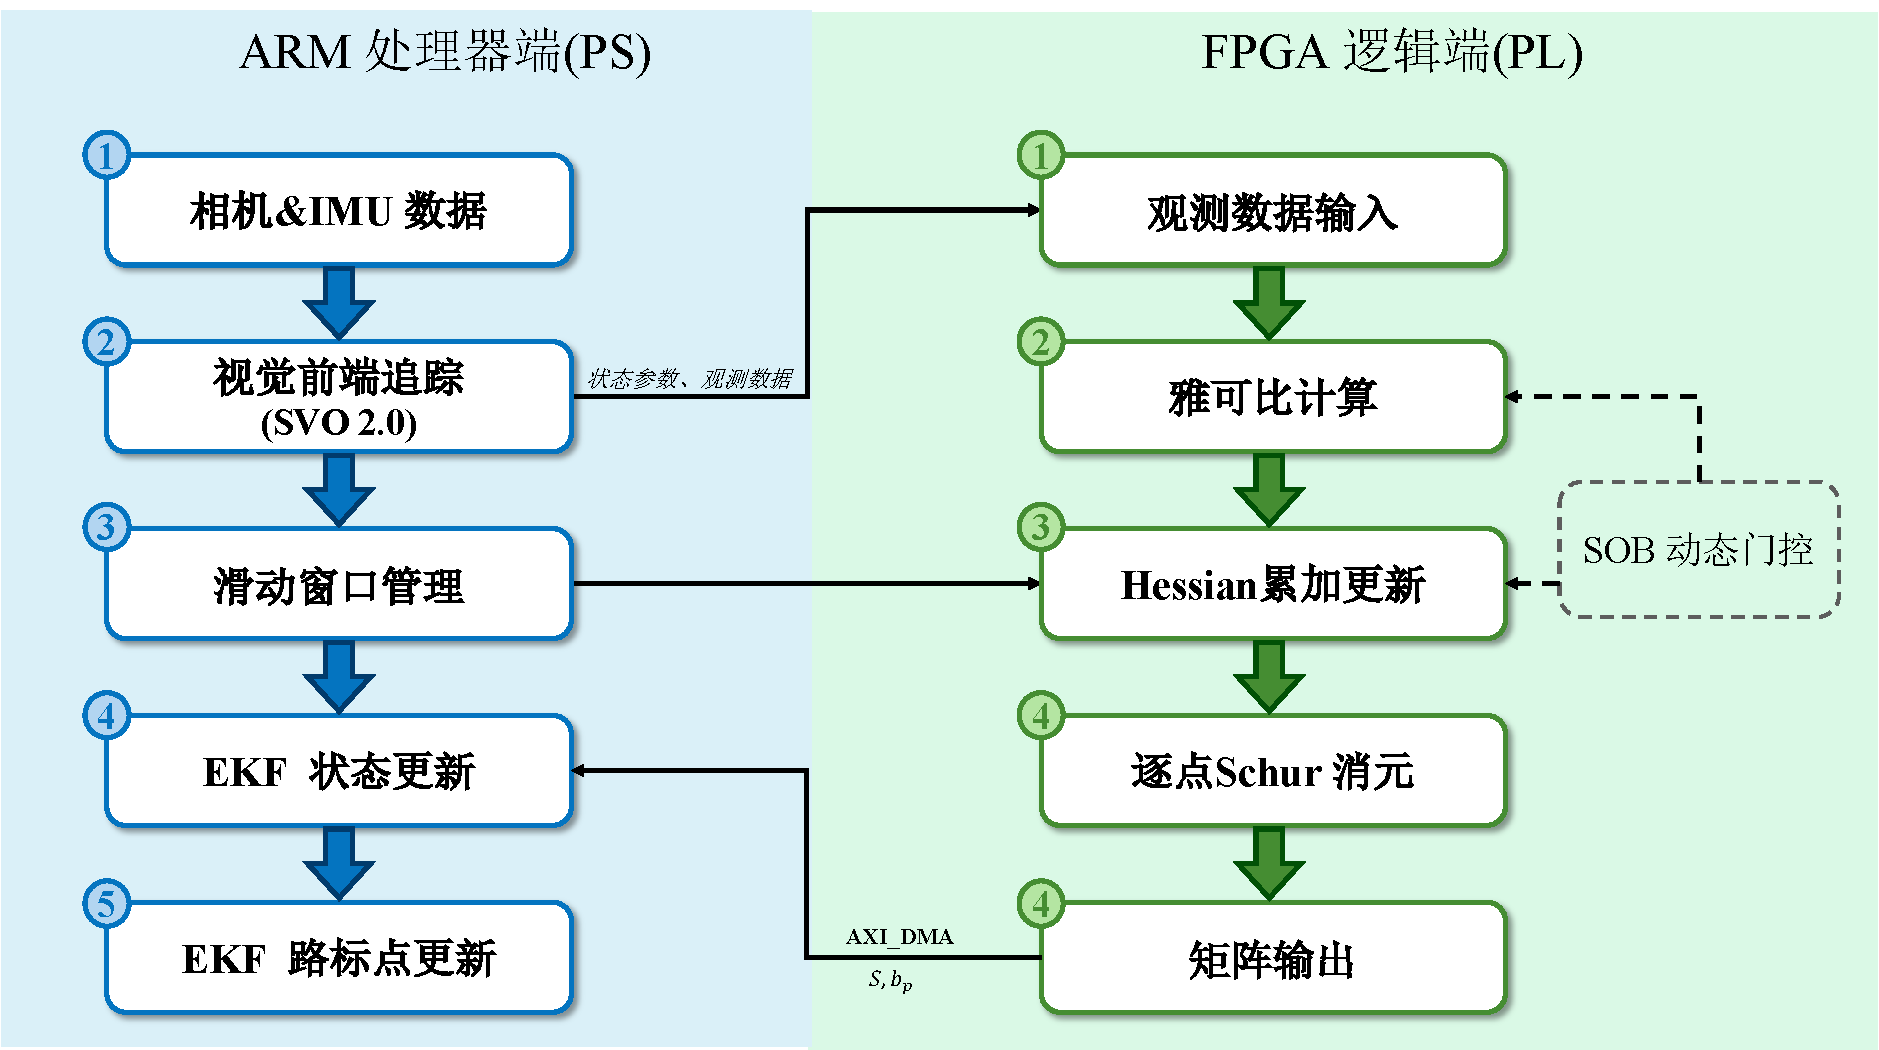
\includegraphics[width=0.95\textwidth]{Img/hw_sw_partition.pdf}
    \bicaption{软硬件功能划分与数据流示意图}{Hardware-Software Functional Partitioning and Data Flow Diagram}
    \label{fig:hw_sw_partition}
\end{figure}

\subsection{ARM 处理器端（PS）任务}

ARM 处理器端主要负责系统的全局协调、低频逻辑评估以及对外部传感器的管理，重点执行具有高逻辑分歧度的非加速任务。其具体任务包括：

\subsubsection{数据获取与多源同步}

系统通过驱动程序实时采集来自双目相机的图像流与惯性测量单元（IMU）的原始加速度计和陀螺仪数据。由于视觉传感器与惯性传感器的采样频率和触发机制存在异步特性（相机通常工作在 20--30~Hz，IMU 则高达 200--400~Hz），系统需要在 PS 端实现精确的时间戳对齐与数据缓冲管理。具体实现上，采用基于硬件时钟的时间戳标注机制，并使用线性插值方法同步异步数据流，确保后续前端追踪与后端优化的观测数据具有时序一致性。

\subsubsection{视觉前端追踪}

本系统采用 SVO 2.0~\cite{forster2017svo} 作为视觉前端，实现快速鲁棒的特征提取与帧间追踪。SVO 2.0 是一种半直接单目视觉里程计（Semi-Direct Monocular Visual Odometry），结合了直接法的快速性与特征法的鲁棒性。其核心工作流程包括以下几个关键步骤：

\paragraph{特征提取与初始化}
系统在新到达的关键帧上执行 FAST（Features from Accelerated Segment Test）角点检测算法，提取图像中具有显著灰度变化的角点特征。为保证特征点在图像上的均匀分布，采用自适应非极大值抑制（Adaptive Non-Maximal Suppression, ANMS）策略，将图像划分为均匀网格并限制每个网格内的特征点数量上限。提取出的特征点被初始化为候选路标点，并建立对应的深度滤波器。

\paragraph{深度滤波与三角化}
由于单目相机缺乏直接的深度信息，系统采用贝叶斯深度滤波器对每个新特征点的逆深度进行概率估计。具体而言，对每个特征点维护一个高斯分布 $\mathcal{N}(\rho, \sigma^2)$，其中 $\rho$ 为逆深度均值，$\sigma^2$ 为不确定性。随着该特征点在后续帧中被持续观测，利用三角测量的几何约束对深度分布进行贝叶斯更新，直至不确定性 $\sigma^2$ 收敛到预设阈值以下，此时该特征点被正式提升为成熟路标点并参与后端优化。

\paragraph{直接法特征对齐}
SVO 2.0 采用基于光度一致性的直接法进行帧间运动估计。对于已跟踪的特征点，系统在当前帧中以其预测投影位置为中心，通过最小化光度残差（Photometric Residual）优化特征点在新帧中的精确像素坐标：
\begin{equation}
    \min_{\mathbf{u}} \sum_{i \in \mathcal{P}} \| I_{\text{ref}}(\mathbf{u}_i) - I_{\text{cur}}(\mathbf{u}_i + \Delta \mathbf{u}) \|^2
\end{equation}
其中 $I_{\text{ref}}$ 和 $I_{\text{cur}}$ 分别为参考帧和当前帧的灰度图像，$\mathcal{P}$ 为特征点邻域的像素集合，$\Delta \mathbf{u}$ 为像素级的位移增量。直接法避免了传统特征描述子的计算开销，显著提升了前端处理速度。

\paragraph{关键帧选择策略}
为防止关键帧冗余并确保滑动窗口内的帧间约束充分，系统采用基于场景覆盖度与视差的关键帧选择策略。当新帧与最近关键帧之间的平均特征点视差超过预设阈值（通常为 5--10 像素），或成功跟踪的特征点比例低于 80\%时，该帧被标记为新关键帧并加入滑动窗口。

\subsubsection{滑动窗口状态管理}

本系统采用基于滑动窗口的状态估计框架，维护固定数量（通常为 4--5 帧）的关键帧状态，以在计算复杂度与估计精度之间取得平衡。滑动窗口内的状态向量定义为：
\begin{equation}
    \mathbf{X} = \begin{bmatrix} \mathbf{x}_0, \mathbf{x}_1, \dots, \mathbf{x}_n \end{bmatrix}^{\mathrm{T}}
\end{equation}
其中每个关键帧状态 $\mathbf{x}_i$ 包含以下分量：
\begin{equation}
    \mathbf{x}_i = \begin{bmatrix} \mathbf{p}_i^{\mathrm{T}}, \mathbf{q}_i^{\mathrm{T}}, \mathbf{v}_i^{\mathrm{T}}, \mathbf{b}_a^{\mathrm{T}}, \mathbf{b}_g^{\mathrm{T}} \end{bmatrix}^{\mathrm{T}}
\end{equation}
\begin{itemize}
    \item $\mathbf{p}_i \in \mathbb{R}^3$：第 $i$ 帧相机在世界坐标系下的位置向量。
    \item $\mathbf{q}_i \in \mathbb{S}^3$：第 $i$ 帧相机的姿态四元数（Quaternion）。
    \item $\mathbf{v}_i \in \mathbb{R}^3$：第 $i$ 帧时刻的三维速度向量。
    \item $\mathbf{b}_a \in \mathbb{R}^3$：加速度计偏差（Accelerometer Bias）。
    \item $\mathbf{b}_g \in \mathbb{R}^3$：陀螺仪偏差（Gyroscope Bias）。
\end{itemize}

当新关键帧加入滑动窗口且窗口已满时，系统需执行边缘化（Marginalization）操作以移除最旧的关键帧。边缘化过程需将被移除帧的观测约束信息保留为先验项，并转化为对剩余状态的约束，从而避免信息丢失。具体实现上，系统通过 Schur 补消元技术将被边缘化状态对应的 Hessian 矩阵块进行消元，并将结果合并到剩余状态的信息矩阵中，保持系统的一致性。

\subsubsection{EKF 位姿与路标点更新}

基于 SchurVINS~\cite{fan2024schurvins} 的设计思想，本系统采用扩展卡尔曼滤波（EKF）框架实现轻量化的状态更新，充分利用 FPGA 端返回的 Schur 消元结果，将位姿优化与路标点更新解耦，极大降低了计算复杂度。

\paragraph{位姿更新}
FPGA 端完成 Schur 消元后，输出降维的位姿相关信息矩阵 $\mathbf{S}$（即更新后的 $\mathbf{H}_{pp}$）和对应的梯度向量 $\mathbf{b}_p'$。这些量构成了仅关于位姿状态的边缘化正规方程：
\begin{equation}
    \mathbf{S} \Delta \mathbf{X}_p = -\mathbf{b}_p'
\end{equation}
其中 $\mathbf{S} = \mathbf{H}_{pp} - \mathbf{H}_{pm}\mathbf{H}_{mm}^{-1}\mathbf{H}_{pm}^{\mathrm{T}}$ 为 Schur 补矩阵，$\Delta \mathbf{X}_p$ 为位姿状态的增量。

在 EKF 框架下，系统将上述信息矩阵视为等效观测模型的雅可比矩阵，并结合先验协方差 $\mathbf{P}$ 计算卡尔曼增益 $\mathbf{K}$：
\begin{equation}
    \mathbf{K} = \mathbf{P} \mathbf{S}^{\mathrm{T}} (\mathbf{S} \mathbf{P} \mathbf{S}^{\mathrm{T}} + \mathbf{R})^{-1}
\end{equation}
其中 $\mathbf{R}$ 为测量噪声协方差矩阵。随后更新位姿状态及其协方差：
\begin{equation}
    \mathbf{X}_p \leftarrow \mathbf{X}_p + \mathbf{K} \mathbf{b}_p'
\end{equation}
\begin{equation}
    \mathbf{P} \leftarrow (\mathbf{I} - \mathbf{K} \mathbf{S}) \mathbf{P}
\end{equation}

由于 Schur 消元已将路标点状态从系统中消去，位姿更新的维度仅为滑动窗口内关键帧状态的总维度（通常为 $15n$，$n$ 为关键帧数量），相比传统的联合优化（包含数百个路标点）计算量降低了一个数量级。

\paragraph{路标点更新}
在位姿状态更新完成后，系统对每个路标点进行独立的增量更新。由于 Schur 消元过程中，路标点与位姿之间的耦合已被解耦，路标点的更新可并行执行。对于第 $k$ 个路标点，其更新梯度为：
\begin{equation}
    \mathbf{b}_{m,k}' = \mathbf{b}_{m,k} - \mathbf{H}_{pm,k}^{\mathrm{T}} \Delta \mathbf{X}_p
\end{equation}
路标点的三维坐标增量 $\Delta \mathbf{x}_{m,k}$ 由下式计算：
\begin{equation}
    \Delta \mathbf{x}_{m,k} = -\mathbf{H}_{mm,k}^{-1} \mathbf{b}_{m,k}'
\end{equation}
其中 $\mathbf{H}_{mm,k}$ 为第 $k$ 个路标点对应的 $3 \times 3$ Hessian 块。由于路标点之间相互独立，该过程可以在 CPU 多线程环境下高效并行化，或借助 FPGA 端预先计算的 $\mathbf{H}_{mm}^{-1}$ 进一步降低计算开销。

通过上述解耦设计，系统实现了增量式的轻量化状态更新，避免了传统基于 Levenberg-Marquardt 迭代求解大规模稀疏线性方程组的高昂开销，为实时性提供了关键保障。

\subsection{FPGA 逻辑端（PL）任务}

FPGA 逻辑端作为协处理器与运算加速核心，利用其大规模并行计算能力处理算法中计算密度最高、数据流规整的稀疏矩阵运算与方程组消元过程。如图~\ref{fig:hw_sw_partition}~右侧所示，其具体任务包括：
\begin{itemize}
    \item \textbf{观测处理与雅可比并行生成}：针对滑动窗口内的视觉观测残差，设计 5 级深度计算流水线，完成从坐标变换、重投影残差计算到关于位姿和路标点的雅可比偏导数（$\mathbf{J}_p$ 和 $\mathbf{J}_m$）的生成计算。
    \item \textbf{Hessian 矩阵块在线累加}：实时将流水线生成的雅可比矩阵进行外积计算，并基于稀疏性累加至片上缓存内的对应 Hessian 块区域（$\mathbf{H}_{pp}, \mathbf{H}_{pm}, \mathbf{H}_{mm}$ 及梯度项 $\mathbf{b}_p, \mathbf{b}_m$）。
    \item \textbf{SOB 编码与动态门控逻辑}：解析经过紧凑编码的稀疏观测位图（SOB），在流水线前端实现数据流旁路（Bypass）与时钟门控（Clock Gating），从而跳过无效的状态与相机块观测运算，提升能效。
    \item \textbf{Schur 消元引擎调度}：在雅可比与 Hessian 矩阵构建完成后，驱动舒尔消元模块高速执行 $3 \times 3$ Hessian 对角块求逆以及基于舒尔补的降维更新操作，输出仅关联相机位姿的简化系统给 PS 端。
\end{itemize}


\section{数据流分析与通信协议设计}

为了有效支撑上述的 PS/PL 异构协同计算架构，必须设计一套与算法流程高度匹配的数据流调度策略以及高效的互联通信协议。

\subsection{系统级数据交互分析}

一次完整的 SLAM 后端优化迭代中的软硬件数据流转可总结为三个主要阶段，具体交互逻辑如图~\ref{fig:ba_core_arch} 所示（详见第~\ref{chap:hardware_design} 章硬件架构设计）：

\begin{enumerate}
    \item \textbf{配置与输入搬运阶段（PS $\rightarrow$ PL）}：
    CPU 在完成前端追踪并决定执行后端优化后，首先将当前滑动窗口的状态参数（包括相机位姿、IMU 预积分增量等）、观测参数（如特征点的像素坐标及有效状态的 SOB 编码）以及路标点的世界坐标等打包。这些数据被放置在双倍数据速率（Double Data Rate, DDR）存储器的指定共享缓存区中。随后，处理器通过控制总线向 PL 侧下发启动命令与地址指针，触发 FPGA 内部的 DMA 读取引擎将上述数据通过突发（Burst）方式读入 PL 内部的多级只读存储器（BRAM）缓冲中。

    \item \textbf{内部流水线计算阶段（PL 内部）}：
    在确保配置与初始数据加载完毕后，FPGA 内部的\textbf{主控制有限状态机（FSM）}接管控制权。首先激活“雅可比计算与 Hessian 累积模块”，从缓冲中连续压入观测与状态数据，驱动 5 级计算流水线。运算产生的稀疏 Hessian 块中间结果写入片上暂存 RAM。当所有路标点的观测均处理完毕，FSM 切换至第二阶段，启动“Schur 消元模块”，从暂存 RAM 中按需读取 $\mathbf{H}_{pm}$ 与 $\mathbf{H}_{mm}$ 进行舒尔补消元更新。由于这两相计算任务共享了大量片间缓存，大幅减少了对片外 DDR 存储器的访存依赖，缓解了传统 SLAM 加速器中常见的存储墙问题。

    \item \textbf{结果回写与系统更新阶段（PL $\rightarrow$ PS）}：
    舒尔消元计算结束时，PL 内部产生经过降维的位姿海森矩阵 $\mathbf{S}$（即舒尔补 $\mathbf{S} = \mathbf{H}_{pp} - \mathbf{H}_{pm}\mathbf{H}_{mm}^{-1}\mathbf{H}_{pm}^{\mathrm{T}}$）和更新后的梯度向量 $\mathbf{b}'_p = \mathbf{b}_p - \mathbf{H}_{pm}\mathbf{H}_{mm}^{-1}\mathbf{b}_m$。主控制 FSM 随即唤醒 DMA 回写引擎，将这部分压缩的矩阵数据写回 DDR 的预期位置。回写完成后，FPGA 向 CPU 触发硬中断信号，通知 PS 端提取计算结果完成后续的卡尔曼增益求解和状态实际更新。
\end{enumerate}

\subsection{PS-PL 通信协议实现}

为保障数据流交互的高带宽和控制请求的低延迟，系统基于先进可扩展接口（Advanced eXtensible Interface, AXI）协议体系设计了异构通信通道：

\begin{itemize}
    \item \textbf{配置与状态监控平面（AXI-Lite）}：
    利用 AXI4-Lite 总线实现轻量级的寄存器级访问。在 FPGA 逻辑侧设计了一组专用的控制与状态寄存器（如 \texttt{IP\_CTRL}、\texttt{IP\_STATUS} 以及基址寄存器）。ARM 处理器通过内存映射 I/O（MMIO）的方式访问这些地址，实现诸如“复位加速器”、“配置基地址”、“启动/停止流水线”等控制动作，并实时诊断 PL 模块状态是否空闲、报错等。

    \item \textbf{大吞吐量数据平面（AXI-MM 与 DMA）}：
    算法所需的观测数据与输出的矩阵规模通常在几兆字节（MB）量级，远超 AXI-Lite 的处理能力。因此系统配置了 AXI4 Memory Mapped（AXI-MM）接口，并在 PL 端实例化了直接存储器访问（DMA）核心。PS 控制端只需下发源地址和目标块大小，数据搬运随即由硬件独立执行。加速器内部还引入了双缓冲（Double Buffering）机制：在计算当前一批数据的同时，DMA 可以预加载接下来需要处理的下一批路标观测特征，实现计算与内存访问延迟的隐藏。

    \item \textbf{事件通知平面（Interrupt）}：
    为避免处理器浪费资源执行休眠轮询（Polling），系统集成了一条连接到 ARM 并行通用中断控制器（GIC）上的直接硬件中断线。每次 DMA 传输完成或整个 Schur Kernel 算法流水终止时，拉高该中断线。在 Linux 或裸机前台的驱动程序响应中断服务例程（ISR）提取数据，从而实现软件任务与硬件执行时间线的完美解耦。
\end{itemize}

\subsection{数据读写时序与双缓冲调度}

为了匹配计算流水线的高速吞吐，避免内存访问成为瓶颈，本系统在数据交互上采用了双缓冲（Double Buffering）或者称作乒乓操作（Ping-Pong Buffer）的队列调度策略。

由于 SLAM 后端优化的工作负载表现出典型的“计算-访存”交替模式，常规的数据提取方式（即等待上一组路标点计算完毕后再发起下一次 DMA 读请求）会导致计算单元的严重空闲。在系统中，片上内存结构被明确划分为两个深度相同的交替使用区域（\texttt{Buffer 0} 与 \texttt{Buffer 1}）。其调度逻辑如下：
当计算单元正在处理 \texttt{Buffer 0} 中已被加载的观测特征和状态变量时，由于外部 AXI 通道仍然处于可用状态，DMA 读取引擎被允许在后台立刻向空闲的 \texttt{Buffer 1} 填充下一次迭代或者下一批路标点的所需数据。一旦计算通道运算完毕且后台加载也就绪，FSM 便会发出交替指令。计算模块立即接入 \texttt{Buffer 1} 进行计算，不仅实现了通信延迟与计算耗时的重叠（Latency Hiding），甚至确保雅可比发生器与 Hessian 累加器的流水线气泡（Stall Bubble）被缩减至最低。

\section{本章小结}

本章从系统顶层视角出发，对基于 Zynq UltraScale+ SoC 的 SLAM 后端加速器进行了整体架构设计，涵盖设计目标确立、软硬件功能划分以及 PS-PL 数据通路与协议设计三个层面，为第四章的硬件模块详细设计提供了系统级依据。

在设计目标方面，本章明确提出四项系统级约束：后端优化频率稳定在 25~Hz 以上以满足实时性需求；利用 FPGA 可定制特性与动态门控机制实现高能效比；通过位宽优化保障硬件计算与全精度软件实现的精度等价性；以及通过 Hessian 紧凑存储与计算复用将核心加速器适配于资源受限的嵌入式 SoC。上述目标共同构成了软硬协同设计的量化指导原则。

在软硬件功能划分方面，本章以逻辑密集型任务归 PS、数据密集型规则计算归 PL 为原则实现深度解耦。PS 端 ARM 处理器负责多传感器数据同步、SVO 2.0 视觉前端追踪（含 FAST 特征提取、光流跟踪与深度滤波）、滑动窗口状态管理（含关键帧选择与边缘化先验更新）以及基于 EKF 框架的轻量化位姿与路标点增量更新；PL 端 FPGA 则专注于观测处理与雅可比并行生成、Hessian 矩阵块在线累加、SOB 编码解析与动态门控，以及 Schur 消元引擎的调度执行。这一划分使得每次后端迭代中计算最密集的雅可比生成与矩阵消元操作完全卸载至硬件流水线，而需要复杂分支判断的状态管理逻辑则保留在处理器端，实现了计算效率与编程灵活性的有机统一。

在数据流与通信协议方面，本章将一次完整后端迭代划分为三个阶段：PS 向 PL 搬运状态、观测与路标数据的配置阶段，FPGA 内部驱动 5 级流水线完成雅可比计算、Hessian 累加与 Schur 消元的计算阶段，以及 PL 将降维后的舒尔补矩阵 $\mathbf{S}$ 与梯度向量 $\mathbf{b}'_p$ 回写 DDR 并触发中断通知 PS 的结果回写阶段。通信层面采用三通道 AXI 架构：AXI4-Lite 实现控制寄存器的低延迟配置与状态监控，AXI4-MM 结合 DMA 引擎实现大吞吐量数据搬运，硬件中断线消除了处理器的轮询等待开销。双缓冲乒乓调度策略进一步将 DMA 预取与流水线计算在时间轴上交叠，有效隐藏了片外存储访问延迟，使计算单元的有效利用率最大化。

\chapter{基于 FPGA 的后端加速器详细设计}\label{chap:hardware_design}

本章详细介绍了基于 FPGA 的 SLAM 后端加速器的具体逻辑设计方案。作为全系统的核心，加速器旨在通过深度流水线化和高度并行的存储架构，实现计算密集型算子的高效执行。本章将依次论述总体硬件架构、Jacobi 处理引擎、基于 SOB 编码的动态门控机制、紧凑型存储管理方案以及舒尔消元核心（Schur Core）的实现细节。

\section{总体硬件架构}

针对后端优化算法的计算特性，本文设计了如图~\ref{fig:ba_core_arch} 所示的 Schur Kernel 硬件加速器架构。该架构采用 PS-PL 异构设计：PS 端的 ARM CPU 负责系统控制与参数配置，通过 AXI-Lite 接口与加速器通信；PL 端实现核心计算逻辑，通过 AXI-MM 直接存储器访问（Direct Memory Access, DMA）接口与双倍数据速率（Double Data Rate, DDR）存储器进行高带宽数据交换。加速器内部划分为两个主要计算模块：Jacobi 计算模块和 Schur 消元模块，分别对应 Hessian 构建阶段与边缘化求解阶段。

\begin{figure}[htbp]
    \centering
    \resizebox{0.95\linewidth}{!}{% BA 硬件加速器架构图
% 使用方法: \input{figures/BA_accelerator_arch.tex}
% 符号与论文 main.tex 保持一致
% 字体: 中文使用宋体（继承文档设置），英文使用 Times New Roman（newtxtext）

\begin{tikzpicture}[
    scale=1.0,
    every node/.append style={font=\rmfamily},  % 确保使用衬线字体（Times/宋体）
    % 模块样式
    mainmodule/.style={draw, thick, rounded corners=3pt, minimum width=2.2cm, minimum height=0.7cm, align=center, font=\small},
    submodule/.style={draw, thick, rounded corners=2pt, minimum width=1.8cm, minimum height=0.6cm, align=center, font=\scriptsize},
    buffer/.style={draw, thick, fill=blue!15, minimum width=1.3cm, minimum height=0.5cm, align=center, font=\scriptsize},
    compute/.style={draw, thick, fill=green!15, rounded corners=2pt, minimum width=1.5cm, minimum height=0.5cm, align=center, font=\scriptsize},
    interface/.style={draw, thick, fill=yellow!25, rounded corners=3pt, minimum width=0.8cm, minimum height=1.8cm, align=center, font=\small},
    phasebox/.style={draw, very thick, rounded corners=5pt, fill=#1, fill opacity=0.08},
    arrow/.style={->, >=stealth, thick},
    dataarrow/.style={->, >=stealth, thick, black},
    ctrlarrow/.style={->, >=stealth, dashed, gray},
]

% ========== 外部接口 (左侧竖排) ==========
\node[interface] (ps) at (-1.2, -2.0) {\rotatebox{90}{PS (ARM) CPU}};
\node[interface, fill=orange!20] (ddr) at (-1.2, -6.8) {\rotatebox{90}{DDR Memory}};

% ========== 加速器边框 ==========
\draw[very thick, rounded corners=6pt, fill=gray!5] (0, 0) rectangle (8.5, -9.0);
\node[anchor=north west, font=\bfseries\small] at (0.2, 0) {Schur Kernel Accelerator (PL)};

% ========== AXI 接口 ==========
\node[submodule, fill=yellow!15, minimum width=1.6cm] (axilite) at (1.2, -2.0) {AXI-Lite\\配置接口};
\node[submodule, fill=yellow!15, minimum width=1.6cm] (aximm) at (1.2, -6.8) {AXI-MM\\DMA};

% 外部连接
\draw[arrow] (ps.east) -- (axilite.west);
\draw[<->, thick] (ddr.east) -- (aximm.west);

% ========== 控制单元 ==========
\node[mainmodule, fill=orange!10, minimum width=1.6cm] (ctrl) at (1.2, -3.6) {主控制\\FSM};
\draw[arrow] (axilite.south) -- (ctrl.north);

% ========== Phase 2 区域 ==========
\draw[phasebox=blue!40] (2.4, -0.6) rectangle (8.2, -4.2);
\node[anchor=north west, font=\scriptsize, blue!70] at (2.6, -0.65) {雅可比计算模块};

% Phase 2 输入缓存
\node[buffer] (sob) at (3.5, -1.45) {SOB 解码器};
\node[buffer] (pts) at (5.3, -1.45) {路标点 $\mathbf{L}_j$};
\node[buffer] (feat) at (7.1, -1.45) {观测 $\mathbf{z}_{ij}$};

% 坐标变换
\node[compute, minimum width=4.2cm] (coord) at (5.3, -2.2) {坐标变换: $\mathbf{p}_w \to \mathbf{p}_i \to \mathbf{p}_c$};

% 残差与雅可比
\node[compute, minimum width=1.6cm] (residual) at (3.9, -2.95) {残差 $\mathbf{r}_{ij}$};
\node[compute, minimum width=2cm] (jacobian) at (6.7, -2.95) {雅可比 $\mathbf{J}_p$, $\mathbf{J}_m$};

% Hessian 累积器
\node[compute, minimum width=4.6cm, fill=cyan!15] (accum) at (5.3, -3.75) {Hessian: $\mathbf{H}_{pp}$, $\mathbf{H}_{pm}$, $\mathbf{H}_{mm}$, $\mathbf{b}_p$, $\mathbf{b}_m$};

% Phase 2 内部连接
\draw[dataarrow] (sob.south) -- (3.5, -1.92);
\draw[dataarrow] (pts.south) -- (5.3, -1.92);
\draw[dataarrow] (feat.south) -- (7.1, -1.92);
\draw[dataarrow] (3.9, -2.48) -- (residual.north);
\draw[dataarrow] (6.7, -2.48) -- (jacobian.north);
\draw[dataarrow] (residual.south) -- (3.9, -3.47);
\draw[dataarrow] (jacobian.south) -- (6.7, -3.47);

% ========== 中间缓存 ==========
\node[buffer, minimum width=4.8cm, fill=purple!15] (interbuf) at (5.3, -5.0) {缓存: $\mathbf{H}_{pp}$, $\mathbf{H}_{pm}$, $\mathbf{H}_{mm}$, $\mathbf{b}_p$, $\mathbf{b}_m$};

% Phase 2 到中间缓存
\draw[dataarrow] (accum.south) -- (interbuf.north);

% ========== Phase 3 区域 ==========
\draw[phasebox=red!40] (2.4, -5.8) rectangle (8.2, -8.1);
\node[anchor=north west, font=\scriptsize, red!70] at (2.6, -5.75) {Schur 消元模块};

% Phase 3 计算模块
\node[compute, fill=red!15, minimum width=1.4cm] (vinv) at (3.5, -6.6) {$\mathbf{H}_{mm}^{-1}$};
\node[compute, fill=red!15, minimum width=1.5cm] (wv) at (5.3, -6.6) {$\mathbf{H}_{pm}\mathbf{H}_{mm}^{-1}$};
\node[compute, fill=red!15, minimum width=1.4cm] (schur) at (7.1, -6.6) {$\mathbf{H}_{pp}$ 更新};

% 输出
\node[buffer, minimum width=4.8cm, fill=green!20] (output) at (5.3, -7.55) {输出: $\mathbf{H}_{pp} - \mathbf{H}_{pm}\mathbf{H}_{mm}^{-1}\mathbf{H}_{pm}^T$};

% Phase 3 内部连接
\draw[dataarrow] (vinv.east) -- (wv.west);
\draw[dataarrow] (wv.east) -- (schur.west);
\draw[dataarrow] (schur.south) -- (7.1, -7.22);

% 中间缓存到 Phase 3
\draw[dataarrow] (interbuf.south) -- (5.3, -5.8);

% ========== DMA 数据流 ==========
% DMA 读取到 Phase 2
\draw[dataarrow] (aximm.east) -- (2.2, -6.8) -- (2.2, -1.45) -- (sob.west);

% 输出写回 DMA
\draw[dataarrow] (output.west) -- (1.2, -7.55) -- (aximm.south);

% 控制信号
\draw[ctrlarrow] (ctrl.east) -- (2.4, -3.6);
\draw[ctrlarrow] (ctrl.south) -- (1.2, -6.0) -- (2.4, -6.0);

% ========== 图例 ==========
% 通过形状区分: 缓存为直角矩形, 计算单元为圆角矩形
\node[font=\scriptsize\bfseries] at (0.37, -8.65) {图例:};
\node[draw, thick, minimum width=0.7cm, minimum height=0.3cm] at (1.3, -8.65) {};
\node[font=\tiny, anchor=west] at (1.7, -8.65) {缓存};
\node[draw, thick, rounded corners=2pt, minimum width=0.7cm, minimum height=0.3cm] at (3.2, -8.65) {};
\node[font=\tiny, anchor=west] at (3.6, -8.65) {计算单元};
\draw[->, >=stealth, thick, black] (5.0, -8.65) -- (5.6, -8.65);
\node[font=\tiny, anchor=west] at (5.7, -8.65) {数据流};
\draw[->, >=stealth, dashed, gray] (6.8, -8.65) -- (7.4, -8.65);
\node[font=\tiny, anchor=west] at (7.5, -8.65) {控制};

\end{tikzpicture}
}
    \bicaption{Schur Kernel 硬件加速器架构}{Architecture of Schur Kernel Hardware Accelerator}
    \label{fig:ba_core_arch}
\end{figure}

\begin{enumerate}
    \item \textbf{Jacobi 计算模块}：如图~\ref{fig:ba_core_arch} 上半部分所示，该模块集成了从原始观测数据到 Hessian 矩阵构建的完整计算流程，主要包含以下子单元：
    \begin{itemize}
        \item \textbf{SOB 解码器}：解析稀疏观测位图（SOB）编码，实现动态门控以跳过无效观测；
        \item \textbf{坐标变换单元}：执行 $\mathbf{p}_w \to \mathbf{p}_i \to \mathbf{p}_c$ 的级联坐标变换，将世界坐标系下的路标点 $\mathbf{L}_j$ 依次变换到 IMU 坐标系和相机坐标系；
        \item \textbf{残差计算单元}：根据相机坐标 $\mathbf{p}_c$ 和观测 $\mathbf{z}_{ij}$ 计算重投影残差 $\mathbf{r}_{ij}$；
        \item \textbf{雅可比生成单元}：采用链式法则计算位姿雅可比矩阵 $\mathbf{J}_p$ 和路标雅可比矩阵 $\mathbf{J}_m$；
        \item \textbf{Hessian 累积器}：执行雅可比矩阵外积运算，在线累积 $\mathbf{H}_{pp}$、$\mathbf{H}_{pm}$、$\mathbf{H}_{mm}$ 以及梯度向量 $\mathbf{b}_p$、$\mathbf{b}_m$。
    \end{itemize}
    \item \textbf{Schur 消元模块}：如图~\ref{fig:ba_core_arch} 下半部分所示，该模块负责将路标点从优化问题中边缘化，输出仅关于位姿的简化系统。其计算流程包含三个流水级：
    \begin{itemize}
        \item \textbf{$\mathbf{H}_{mm}^{-1}$ 计算}：利用 $\mathbf{H}_{mm}$ 的块对角特性，采用解析公式直接计算每个 $3\times3$ 子块的逆；
        \item \textbf{$\mathbf{H}_{pm}\mathbf{H}_{mm}^{-1}$ 计算}：对每个有效的状态-路标关联对，计算中间矩阵积；
        \item \textbf{$\mathbf{H}_{pp}$ 更新}：执行舒尔补累加，输出 $\mathbf{H}_{pp} - \mathbf{H}_{pm}\mathbf{H}_{mm}^{-1}\mathbf{H}_{pm}^{\mathrm{T}}$。
    \end{itemize}
\end{enumerate}

\section{Jacobi 处理引擎设计}

\subsection{模块层次与数据依赖}

为保证流水线的高吞吐与低延迟，硬件设计首先明确模块之间的数据依赖关系，并据此划分层次结构。图~\ref{fig:data_dependency} 展示了从输入数据到 Hessian 累积、再到 Schur 消元的关键依赖链路：状态四元数与位置、路标点坐标与相机内参共同决定坐标变换结果 $\mathbf{P}_c$，其进一步驱动残差 $\mathbf{r}$ 与雅可比矩阵 $\mathbf{J}_p, \mathbf{J}_m$ 的生成；在此基础上累积 $\mathbf{A}, \mathbf{b}, \mathbf{V}, \mathbf{g}, \mathbf{W}$ 等中间量，待 Phase2 完成后才能进入 Schur 消元阶段。这一依赖关系确保了“观测独立—点内串行—点间并行”的调度原则。

图~\ref{fig:module_hierarchy} 给出了 Schur Kernel 的模块层次结构，从顶层控制到输入缓冲、坐标变换、雅可比计算、Hessian 累积、Schur 消元及输出缓冲，形成清晰的层次化组织。该结构既便于调试，也有利于后续在不同 FPGA 平台上的资源裁剪与复用。

\begin{figure}[htbp]
    \centering
    \resizebox{0.92\linewidth}{!}{% 数据依赖图
% 使用方法: 在主文档中 \input{figures/data_dependency.tex}
% 字体: 中文使用宋体（继承文档设置），英文使用 Times New Roman（newtxtext）

\begin{tikzpicture}[
    every node/.append style={font=\rmfamily},  % 确保使用衬线字体（Times/宋体）
    data/.style={draw, thick, rounded corners=3pt, fill=blue!10, minimum width=1.8cm, minimum height=0.6cm, align=center, font=\footnotesize},
    proc/.style={draw, thick, rounded corners=3pt, fill=green!15, minimum width=2.2cm, minimum height=0.7cm, align=center, font=\footnotesize},
    output/.style={draw, thick, rounded corners=3pt, fill=orange!15, minimum width=1.5cm, minimum height=0.6cm, align=center, font=\footnotesize},
    final/.style={draw, thick, rounded corners=3pt, fill=red!15, minimum width=2.5cm, minimum height=0.7cm, align=center, font=\footnotesize},
    arrow/.style={->, >=stealth, thick},
    group_box/.style={draw, dashed, thick, rounded corners=5pt},
]

% ========== 输入数据 ==========
\node[data] (state_quat) at (0, 0) {状态姿态\\参数};
\node[data] (state_pos) at (0, -1) {状态位置\\参数};
\node[data] (pts_pw) at (0, -2) {路标点\\世界坐标};
\node[data] (intrin) at (0, -3) {内参\\参数};

\node[group_box, fit=(state_quat)(state_pos)(pts_pw)(intrin), inner sep=5pt] (input_box) {};
\node[anchor=south, font=\scriptsize\bfseries] at (input_box.north) {输入数据};

% ========== 坐标变换 ==========
\node[proc] (coord_trans) at (4, -1.5) {坐标变换\\$\mathbf{P}_w \to \mathbf{P}_c$};

\draw[arrow] (state_quat) -- (coord_trans);
\draw[arrow] (state_pos) -- (coord_trans);
\draw[arrow] (pts_pw) -- (coord_trans);
\draw[arrow] (intrin) -- (coord_trans);

% ========== 残差计算 ==========
\node[output] (Pc) at (7, -1) {$\mathbf{P}_c$};
\node[proc] (residual) at (10, -1) {残差计算};
\node[output] (r) at (13, -1) {$\mathbf{r}$};

\draw[arrow] (coord_trans) -- (Pc);
\draw[arrow] (Pc) -- (residual);
\draw[arrow] (residual) -- (r);

% ========== 雅可比计算 ==========
\node[proc] (jacobian) at (7, -3) {雅可比计算};

\draw[arrow] (Pc) -- (jacobian);
\draw[arrow] (coord_trans) |- (jacobian);

% ========== 雅可比输出 ==========
\node[output] (jx) at (4, -4.5) {$\mathbf{J}_p$};
\node[output] (jf) at (7, -4.5) {$\mathbf{J}_m$};
\node[output] (dr_dpc) at (10, -4.5) {$\frac{\partial r}{\partial p_c}$};

\draw[arrow] (jacobian) -- (jx);
\draw[arrow] (jacobian) -- (jf);
\draw[arrow] (jacobian) -- (dr_dpc);

% ========== Hessian 累积更新 ==========
\node[group_box, minimum width=10cm, minimum height=1.8cm, fill=yellow!5] (hessian_box) at (7, -6.5) {};
\node[anchor=north, font=\scriptsize\bfseries] at (7, -5.7) {Hessian 累积更新};

\node[output] (A) at (3.5, -6.8) {$\mathbf{H}_{pp}$\\(累加)};
\node[output] (b) at (5.5, -6.8) {$\mathbf{b}_p$\\(累加)};
\node[output] (V) at (7.5, -6.8) {$\mathbf{H}_{mm}$\\(累加)};
\node[output] (g) at (9.5, -6.8) {$\mathbf{b}_m$\\(累加)};

\draw[arrow] (jx) -- (A);
\draw[arrow] (jx) -- (b);
\draw[arrow] (r.south) -- ++(0, -1) -| (b);
\draw[arrow] (jf) -- (V);
\draw[arrow] (jf) -- (g);
\draw[arrow] (r.south) -- ++(0, -1) -| (g);

% H_{pm} 矩阵
\node[output] (W) at (11.5, -6.8) {$\mathbf{H}_{pm}$};
\draw[arrow] (jx.south) -- ++(0, -0.5) -| (W);
\draw[arrow] (jf.south) -- ++(0, -0.5) -| (W);

% ========== Schur 消元 ==========
\node[final] (schur) at (7, -8.5) {Schur消元\\等待 Hessian 累积完成};

\draw[arrow] (A) -- (schur);
\draw[arrow] (b) -- (schur);
\draw[arrow] (V) -- (schur);
\draw[arrow] (g) -- (schur);
\draw[arrow] (W) -- (schur);

% ========== 最终输出 ==========
\node[final, fill=green!20] (output) at (7, -10) {$\mathbf{S}, \mathbf{b}'_p$\\(输出)};

\draw[arrow] (schur) -- (output);

\end{tikzpicture}
}
    \bicaption{Jacobi 计算与 Schur 消元的数据依赖关系}{Data dependency across Jacobian generation and Schur elimination}
    \label{fig:data_dependency}
\end{figure}

\begin{figure}[htbp]
    \centering
    \resizebox{0.88\linewidth}{!}{% 模块层次结构图
% 使用方法: 在主文档中 \input{figures/module_hierarchy.tex}
% 字体: 中文使用宋体（继承文档设置），英文使用 Times New Roman（newtxtext）

\begin{tikzpicture}[
    every node/.append style={font=\rmfamily},  % 确保使用衬线字体（Times/宋体）
    level 1/.style={sibling distance=3.8cm, level distance=1.5cm},
    level 2/.style={sibling distance=1.8cm, level distance=1.3cm},
    level 3/.style={sibling distance=1.5cm, level distance=1.2cm},
    module/.style={draw, thick, rounded corners=2pt, fill=blue!10, minimum width=1.8cm, minimum height=0.6cm, align=center, font=\tiny},
    submodule/.style={draw, rounded corners=2pt, fill=green!10, minimum width=1.4cm, minimum height=0.5cm, align=center, font=\tiny},
    leaf/.style={draw, rounded corners=2pt, fill=yellow!10, minimum width=1.2cm, minimum height=0.4cm, align=center, font=\tiny},
    edge from parent/.style={draw, thick, ->,>=stealth},
]

\node[module, minimum width=3cm, fill=blue!20] (top) {schur\_kernel\_top}
    child {node[module] {axi\_lite\_slave}
        child {node[submodule] {register\_file}}
    }
    child {node[module] {axi\_mm\_master}
        child {node[submodule] {read\_engine}}
        child {node[submodule] {write\_engine}}
    }
    child {node[module] {main\_fsm}}
    child {node[module] {input\_buffer}
        child {node[leaf] {state\_param\_buf}}
        child {node[leaf] {sob\_buf}}
        child {node[leaf] {pts\_pw\_buf}}
        child {node[leaf] {feature\_uv\_buf}}
    }
    child {node[module] {coord\_transform\_unit}
        child {node[leaf] {quat\_mult}}
        child {node[leaf] {quat\_conj}}
        child {node[leaf] {quat\_rotate}}
        child {node[leaf] {quat\_to\_rotmat}}
        child {node[leaf] {mat3x3\_mult}}
    }
    child {node[module] {jacobian\_unit}
        child {node[leaf] {residual\_calc}}
        child {node[leaf] {huber\_scale}}
        child {node[leaf] {dr\_dpc\_calc}}
        child {node[leaf] {dpc\_dpos\_calc}}
        child {node[leaf] {jx\_calc}}
        child {node[leaf] {jf\_calc}}
    }
    child {node[module] {hessian\_accum\_unit}
        child {node[leaf] {jxT\_jx\_accum}}
        child {node[leaf] {jfT\_jf\_accum}}
        child {node[leaf] {jxT\_jf\_store}}
        child {node[leaf] {jxT\_r\_accum}}
        child {node[leaf] {jfT\_r\_accum}}
    }
    child {node[module] {intermediate\_buffer}
        child {node[leaf] {tmp\_amtx\_buf}}
        child {node[leaf] {tmp\_bvct\_buf}}
        child {node[leaf] {tmp\_v\_buf}}
        child {node[leaf] {tmp\_gv\_buf}}
        child {node[leaf] {tmp\_w\_buf}}
    }
    child {node[module] {schur\_elim\_unit}
        child {node[leaf] {mat3x3\_inv}}
        child {node[leaf] {w\_vinv\_mult}}
        child {node[leaf] {wvinv\_wT\_mult}}
        child {node[leaf] {wvinv\_g\_mult}}
        child {node[leaf] {a\_update}}
    }
    child {node[module] {output\_buffer}}
    child {node[module] {fp64\_unit}
        child {node[leaf] {fp64\_add[N]}}
        child {node[leaf] {fp64\_mul[M]}}
        child {node[leaf] {fp64\_div}}
        child {node[leaf] {fp64\_sqrt}}
    };

\end{tikzpicture}
}
    \bicaption{Schur Kernel 硬件模块层次结构}{Module hierarchy of the Schur Kernel accelerator}
    \label{fig:module_hierarchy}
\end{figure}

Jacobi 矩阵的生成是后端优化中计算量最大的环节之一。在本系统中，Jacobi 处理引擎（JPE）负责计算视觉观测残差 $\mathbf{r}$ 对载体位姿 $\mathbf{p}$ 和路标点坐标 $\mathbf{m}$ 的偏导数。为实现高吞吐率与低延迟，JPE 采用 5 级深度流水线并行处理，同时在输入侧与 SOB 解码器耦合，形成“观测判定—流水计算—稀疏累加”的完整数据通路。

\subsection{5 级流水线架构}

雅可比偏导数的计算涉及复杂的坐标系转换与链式法则求导。为最大化吞吐量，JPE 采用 5 级深度流水线架构，通过时间交叠方式同时处理多组观测，显著提升计算效率。各级功能详解如下（对应观测处理流水线如图~\ref{fig:obs_pipeline} 所示）：

\begin{itemize}
    \item \textbf{Stage 1：IMU 坐标系变换与预计算级}。包含两条并行逻辑：(A) 通过坐标差分与四元数旋转电路，将世界坐标系下的路标点 $\mathbf{p}_w$ 变换为 IMU 坐标系下的坐标 $\mathbf{p}_i = \mathbf{q}_{st} \otimes (\mathbf{p}_w - \mathbf{t}_{st})$，其中 $\mathbf{q}_{st}$ 与 $\mathbf{t}_{st}$ 分别为待优化状态位姿的旋转四元数与平移向量，$\otimes$ 表示四元数旋转算子；(B) 同步计算状态旋转矩阵 $\mathbf{R}_{st}$、IMU 点的反对称矩阵 $\mathbf{p}_i^{\wedge}$（其中 $(\cdot)^{\wedge}$ 为将三维向量映射为反对称矩阵的算符，用于表示叉积运算）以及相机-世界旋转矩阵 $\mathbf{R}_{cw}$，为后续链式法则提供中间变量。
    \item \textbf{Stage 2：相机坐标系投影与中间矩阵计算级}。利用外参 $(\mathbf{t}_{ic}, \mathbf{q}_{ic})$ 将 IMU 坐标 $\mathbf{p}_i$ 变换为相机坐标系下的坐标 $\mathbf{p}_c$。同时，配置专用矩阵乘法单元，并行计算 $\mathbf{R}_{ic} \mathbf{p}_i^{\wedge} \mathbf{R}_{st}^{\mathrm{T}}$，其中 $\mathbf{R}_{ic}$ 为由外参 $\mathbf{q}_{ic}$ 转换得到的 IMU 到相机的旋转矩阵。这一项是后续求解位姿导数的关键公共因子。
    \item \textbf{Stage 3：链式法则中间导数计算级}。专注于偏导数的分解计算，降低单级逻辑深度以保证高频运行。结合观测特征点坐标 $(u, v)$ 和预测坐标 $\mathbf{p}_c$，分别计算残差关于相机系坐标点的偏导数 $\partial\mathbf{r}/\partial\mathbf{p}_c$ 和相机系坐标点关于状态位姿的偏导数 $\partial\mathbf{p}_c/\partial\mathbf{x}$。
    \item \textbf{Stage 4：雅可比生成级}。作为导数计算的汇聚点，利用 Stage 3 的中间导数与 Stage 1 的 $\mathbf{R}_{cw}$ 进行组合，并行输出重投影误差对状态位姿的雅可比矩阵 $\mathbf{J}_p$ 和对路标点的雅可比矩阵 $\mathbf{J}_m$。
    \item \textbf{Stage 5：海森累加级}。在流水线末端，配置矩阵乘加阵列执行雅可比矩阵的外积运算 $\mathbf{H} = \mathbf{J}^{\mathrm{T}} \mathbf{W} \mathbf{J}$，将结果直接累加到片上缓存（BRAM）对应的 Hessian 子块（$\mathbf{H}_{pp}, \mathbf{H}_{pm}, \mathbf{H}_{mm}$）中。
\end{itemize}

\subsection{定点化精度优化}

由于 FPGA 对浮点运算的支持成本较高，JPE 全面采用了定点数进行计算。通过对 EuRoC 数据集的仿真分析，本文采用了 Q16.16 的定点格式用于中间雅可比项，而对于路标点逆深度等敏感分量采用了更高的精度保护。实验表明，相比于双精度浮点实现，该定点化方案引入的位姿估计误差低于 0.5\%。

\section{SOB 编码与动态门控机制实现}

为了最大化能效比，加速器利用了 VIO 系统中观测的天然稀疏性。Hessian 矩阵的 $\mathbf{H}_{pm}$ 子块呈现高度不规则的稀疏结构，这源于观测的局部性——一个路标点仅被滑动窗口内少数相机观测到。传统稠密矩阵存储会导致大量零元素占用资源；而通用的 CSR（压缩稀疏行）格式虽能节省存储，但其复杂的索引数组解析会显著增加硬件控制的复杂度与延迟。为此，本系统引入稀疏观测位图（Sparse Observation Bitmap, SOB）编码，将观测拓扑压缩为定长位图，通过位运算直接驱动流水线调度与门控控制。

\subsection{SOB 位定义与编码格式}

本文采用 8 位 SOB 向量对单个路标点在滑动窗口内的观测活跃情况进行编码。设窗口内包含 4 个状态（从旧到新编号为 State 0$\sim$3，对应 $S_1$--$S_4$），每个状态对应左右双目两路观测，则 SOB 位序定义为：
\begin{equation}
    \text{SOB} = [b_7,b_6,b_5,b_4,b_3,b_2,b_1,b_0]
\end{equation}
位序映射关系为：Bit [7:6] $\rightarrow$ State 3（右目/左目），Bit [5:4] $\rightarrow$ State 2（右目/左目），Bit [3:2] $\rightarrow$ State 1（右目/左目），Bit [1:0] $\rightarrow$ State 0（右目/左目）。比特值为 0 表示无观测（对应 $\mathbf{H}_{pm}$ 中的零子块），比特值为 1 表示有效观测（对应非零的 $6\times3$ 有效块）。该编码与特征点数据包同时传输，使硬件能够在进入 Jacobi 计算前完成零块判定并建立观测拓扑。

\begin{figure}[htbp]
    \centering
    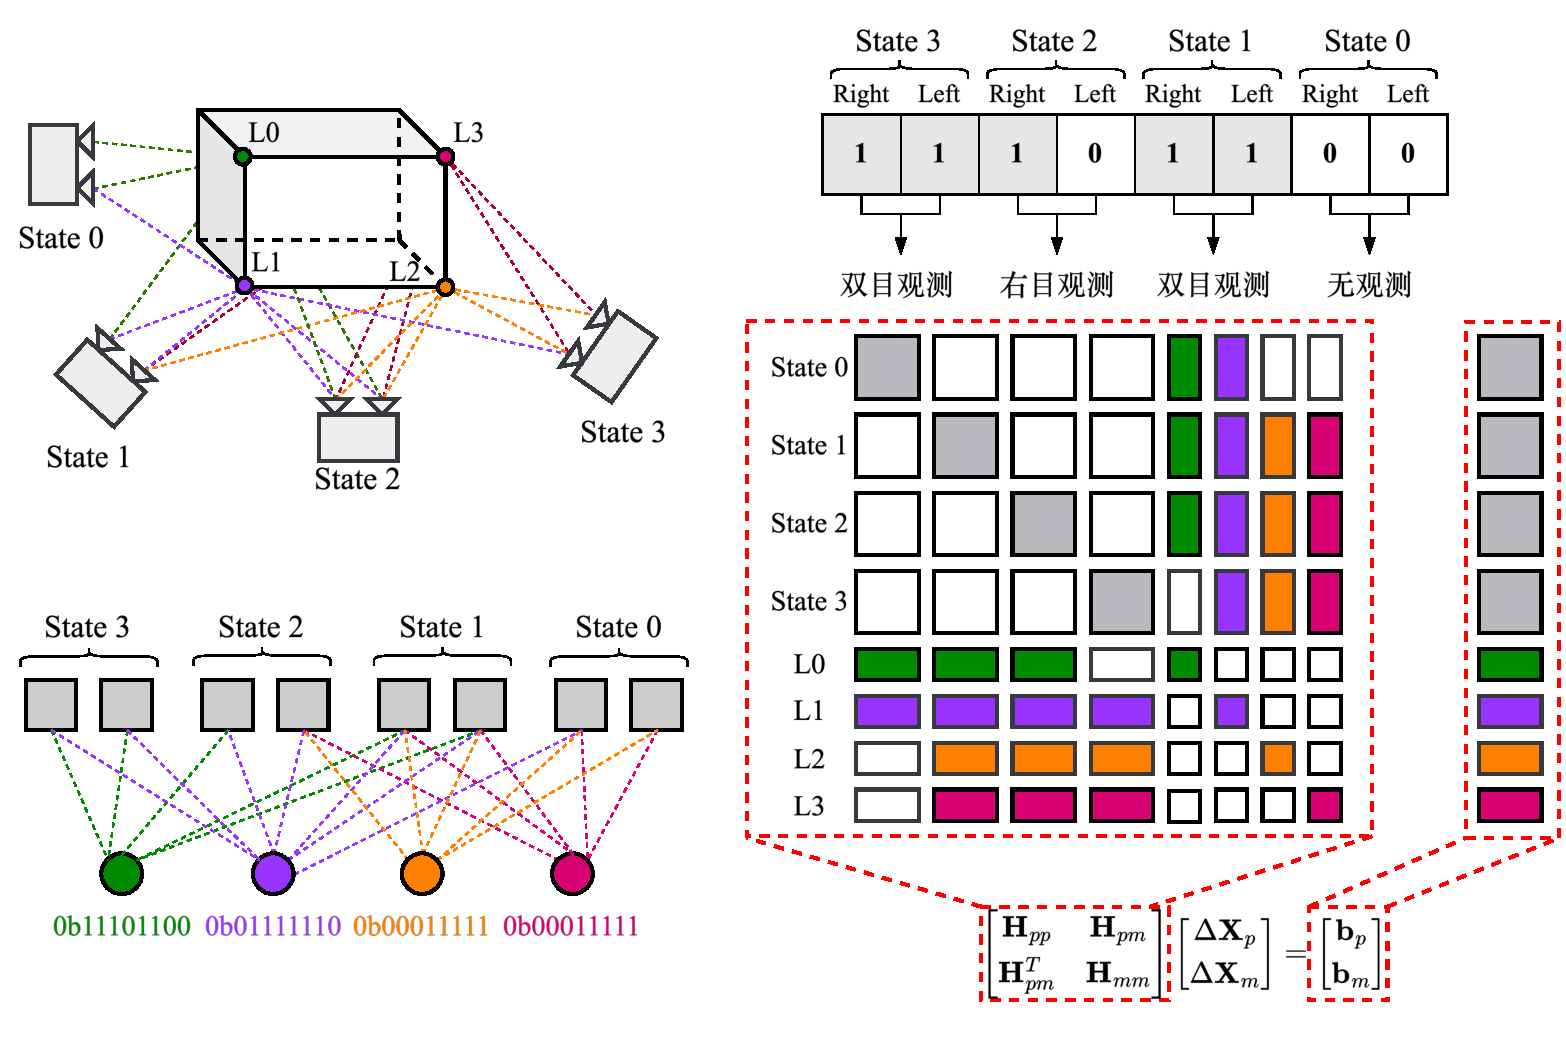
\includegraphics[width=0.78\textwidth]{Img/Observation.pdf}
    \bicaption{稀疏观测位图（SOB）编码示意}{Illustration of Sparse Observation Bitmap (SOB) encoding}
    \label{fig:sob_encoding}
\end{figure}

例如，若某路标点的 SOB 编码为 \texttt{0b11101100}，表示该点仅被 State 1 的双目相机、State 2 的右目相机以及 State 3 的双目相机观测到。在构建 Hessian 矩阵时，系统据此仅对 5 个有效观测开启计算逻辑执行雅可比生成与矩阵累加，而对其余 3 个无效观测（零块）直接执行时钟阻断，从而有效规避不必要的计算开销。

\subsection{SOB 解析逻辑电路}

SOB 解析模块位于 Jacobi 引擎的前端。对于每个传入的路标点包，模块首先提取其携带的 8 位 SOB 正则码，并据此完成观测筛选与流水线调度。观测处理流水线与稀疏累加流程如图~\ref{fig:obs_pipeline} 所示。
\begin{enumerate}
    \item \textbf{高效状态掩码}：通过一组并行的与门（AND Gate）阵列，计算每一位对应的有效性。
    \item \textbf{零块预测器}：当状态对应的两位 $b_{2i+1}$ 和 $b_{2i}$ 均为 0 时，预测器产生一个 \texttt{SKIP\_STATE} 信号。
\end{enumerate}

\begin{figure}[htbp]
    \centering
    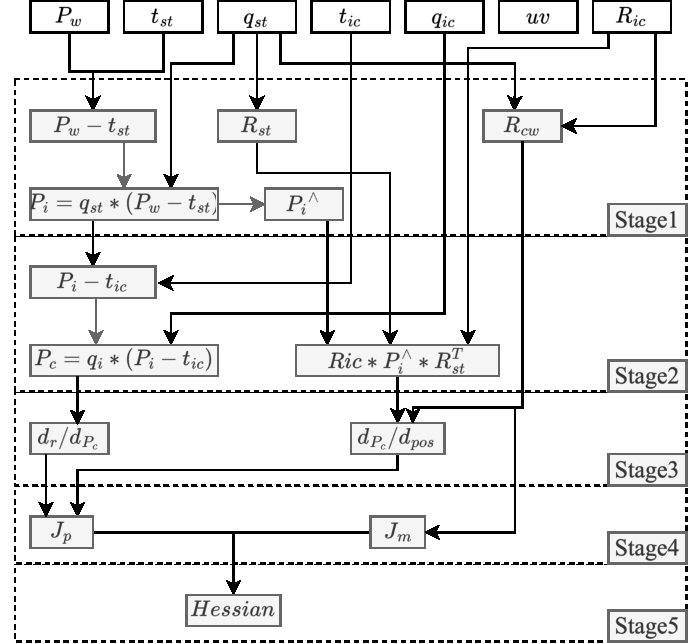
\includegraphics[width=0.86\textwidth]{Img/Hessian-build-pipe.pdf}
    \bicaption{观测处理流水线与稀疏累加流程示意}{Observation processing pipeline and sparse accumulation flow}
    \label{fig:obs_pipeline}
\end{figure}

\subsection{动态时钟门控机制}

为了将稀疏性转化为实际的功耗与速度优势，流水线输入端耦合有稀疏编码解码与判决逻辑。该逻辑根据 SOB 位特征，在硬件底层执行两级动态门控：
\begin{itemize}
    \item \textbf{第一级门控（状态级旁路）}：判决逻辑首先检查代表当前状态（State）的 2 位编码组合（对应左右相机）。若两位均为逻辑“0”（即 \texttt{0b00}），表明该路标点在该时刻完全不可见。此时控制逻辑向 Stage 1 发送旁路信号，直接跳过“世界坐标系到 IMU 坐标系”的刚体变换（包括四元数旋转与平移减法电路），流水线不发生数据翻转。
    \item \textbf{第二级门控（相机级时钟阻断）}：当数据进入后续级数时，判决逻辑进一步检查当前处理相机的独立编码位。若该位为逻辑“0”，表明该特定相机无观测数据。此时控制逻辑向 Stage 2 至 Stage 5 发送时钟门控信号（Clock Gating）：
    \begin{itemize}
        \item \textbf{跳过 Stage 2}：阻断“IMU 系到相机系”的坐标变换及投影计算电路；
        \item \textbf{跳过 Stage 3--4}：阻断雅可比矩阵（$\mathbf{J}_p, \mathbf{J}_m$）的偏导数乘法器时钟；
        \item \textbf{跳过 Stage 5}：阻断 Hessian 矩阵外积（$\mathbf{J}^{\mathrm{T}}\mathbf{J}$）的累加器时钟。
    \end{itemize}
\end{itemize}

为了避免频繁开关时钟造成时序抖动，控制逻辑对 SOB 信号进行了双级寄存器同步，并在状态切换边界插入保护周期（Guard Cycle）。当某一状态的两位均为 0 时，系统不仅跳过该状态的 Jacobi 计算，还会阻断对应 Hessian 块的写入，从而实现“计算—存储”一致的门控策略。通过这种“粗细结合”的门控机制，硬件加速器不仅消除了无效数据的存储访问，更在物理层面完全切断了无效计算路径的动态功耗，实现了计算量与观测稀疏度的线性相关。实验测得在稀疏观测序列中，该机制可降低约 35\% 的动态功耗，如图~\ref{fig:sob_reduction} 所示。

\begin{figure}[htbp]
    \centering
    \resizebox{0.75\textwidth}{!}{% SOB 编码计算量优化效果 - 折线图
% 使用方法: \input{figures/sob_computation_chart.tex}
% 字体: 中文使用宋体（继承文档设置），英文使用 Times New Roman（newtxtext）

\usetikzlibrary{arrows.meta}
\begin{tikzpicture}
\begin{axis}[
    every node/.append style={font=\rmfamily},  % 确保使用衬线字体（Times/宋体）
    width=0.85\linewidth,
    height=5.5cm,
    xlabel={稀疏率 (\%)},
    ylabel={迭代次数},
    xmin=30, xmax=80,
    ymin=0, ymax=2200,
    xtick={37.5, 50, 62.5, 73.2},
    legend pos=north west,
    legend style={font=\small},
    grid=major,
    grid style={dashed, gray!30},
    axis lines=left,
    xlabel style={font=\small},
    ylabel style={font=\small},
    tick label style={font=\small},
]

% 朴素迭代 - 蓝色实线
\addplot[
    color=blue,
    mark=square*,
    thick,
    mark size=3pt,
] coordinates {
    (37.5, 400)
    (50.0, 1200)
    (62.5, 1600)
    (73.2, 2048)
};
\addlegendentry{朴素迭代}

% 优化迭代 - 红色虚线
\addplot[
    color=red,
    mark=triangle*,
    thick,
    dashed,
    mark size=3pt,
] coordinates {
    (37.5, 152)
    (50.0, 600)
    (62.5, 974)
    (73.2, 1433)
};
\addlegendentry{SOB 优化迭代}

\end{axis}
\end{tikzpicture}
}
    \bicaption{SOB 编码带来的计算量优化效果}{Computation reduction achieved by SOB encoding}
    \label{fig:sob_reduction}
\end{figure}

\subsection{数据与索引分离存储}

针对 $\mathbf{H}_{pm}$ 矩阵子块呈现出的高度不规则稀疏特性，传统的块稀疏行（BSR）或压缩稀疏列（CSC）格式\cite{saad2003iterative}需要显式存储大量的行/列索引数组，不仅占用了额外的存储空间，还增加了硬件地址生成单元的逻辑复杂度。为此，本文利用前述的 SOB 编码，提出了一种“隐式索引”存储优化策略，将数据存储与拓扑结构完全解耦：
\begin{itemize}
    \item \textbf{紧凑数据流（Compact Data Stream）}：鉴于有效观测的稀疏性，系统在片上存储器（BRAM/URAM）中开辟连续的存储空间，仅按顺序紧凑存储非零的有效 Hessian 子块（$6\times3$ 维度）。这种存储方式完全摒弃了零元素的物理存储，实现了“数据即满”，最大化了存储资源的利用率与访存带宽。
    \item \textbf{隐式索引流（Implicit Indexing Stream）}：系统不再维护独立的显式索引表，而是直接复用路标点的 SOB 编码作为元数据索引。硬件解码逻辑通过对掩码执行种群计数（Population Count）指令\cite{warren2013hacker}，即可实时计算出当前路标点对应的有效数据块偏移量与总数；通过检测掩码中“1”的位位置，即可动态解析出每个数据块在逻辑上从属的相机位姿行索引。这种设计将复杂的稀疏矩阵索引操作转化为低延迟的位逻辑运算，确保舒尔消元过程中 $\mathbf{H}_{pm}\mathbf{H}_{mm}^{-1}\mathbf{H}_{pm}^{\mathrm{T}}$ 运算的精确行列对齐。
\end{itemize}


\section{存储管理与 BRAM 优化}

在 Zynq 平台上，片上块存储（BRAM）是非常宝贵的硬件资源。本系统的设计目标是将全滑动窗口的 Hessian 矩阵存储开销控制在 80~KB 以内。为此，系统在存储架构上同时采用“稀疏块压缩 + 数据与索引解耦”的策略，并通过双端口与乒乓缓存机制隐藏访存延迟。此外，PL 端通过 AXI-MM 与 DDR 建立高带宽通路，观测输入与 Schur 输出均采用 DMA 流式传输，从而保证流水线与外部存储节拍匹配。

\subsection{紧凑型 Hessian 存储结构}

由于 $\mathbf{H}_{mm}$ 为块对角矩阵且 $\mathbf{H}_{pm}$ 极其稀疏，系统不再存储完整的密集矩阵，而采用紧凑稀疏块存储方式：
\begin{enumerate}
    \item \textbf{非零块打包}：仅为观测活跃的索引分配存储空间。每个有效的 $6\times3$ 子块采用顺序线性布局，避免零块占用物理地址。
    \item \textbf{隐式索引寻址}：利用 SOB 编码的位索引作为存储地址的一部分，消除了显式索引查找表所需的额外 BRAM；同时与前述“隐式索引流”一致，保证数据流与控制流同步。
\end{enumerate}

\subsection{数据对齐与乒乓缓存}

为支撑 Schur 核心模块的高速运行，Hessian 存储器采用双端口（Dual-port）结构，并实现一套乒乓缓存（Ping-pong Buffer）机制。硬件在计算当前路标点的同时，可将上一路标点的中间更新结果写回，从而隐藏存储器访问延迟。与此同时，输入数据流在片上按固定宽度对齐，确保与 DMA 传输和流水线节拍一致，降低仲裁与跨时钟域同步的开销。

\subsection{主控制 FSM 与数据流调度}

为保证“加载—计算—写回”过程稳定有序，加速器内部设计了主控制状态机（FSM），其状态转移与流水线执行关系如图~\ref{fig:main_fsm} 所示。FSM 从 \texttt{IDLE} 状态响应启动信号，依次完成参数加载（\texttt{LOAD\_PARAMS}）、观测与位图并行读取（\texttt{LOAD\_INPUTS}），随后进入 Phase2/Phase3 计算循环，并在完成 Schur 更新后通过 DMA 写回结果，最终回到空闲状态等待下一帧。

\begin{figure}[htbp]
    \centering
    \resizebox{0.88\linewidth}{!}{% 主控制状态机 FSM 图
% 使用方法: 在主文档中 \input{figures/main_fsm.tex}
% 字体: 中文使用宋体（继承文档设置），英文使用 Times New Roman（newtxtext）

\begin{tikzpicture}[
    every node/.append style={font=\rmfamily},  % 确保使用衬线字体（Times/宋体）
    state/.style={draw, thick, rounded corners=5pt, minimum width=2.6cm, minimum height=0.9cm, align=center, font=\footnotesize},
    state_idle/.style={state, fill=gray!20},
    state_load/.style={state, fill=blue!15},
    state_phase2/.style={state, fill=green!15},
    state_phase3/.style={state, fill=orange!15},
    state_write/.style={state, fill=purple!15},
    state_done/.style={state, fill=yellow!20},
    arrow/.style={->, >=Stealth, thick},
    condition/.style={font=\tiny, align=center},
    loop_box/.style={draw, dashed, thick, rounded corners=8pt, fill=white, fill opacity=0.7},
]

% ========== 状态节点 ==========
\node[state_idle] (idle) at (0, 0) {IDLE};

\node[state_load] (load_param) at (0, -1.8) {LOAD\_PARAMS\\读取参数};

\node[state_load] (load_input) at (0, -3.6) {LOAD\_INPUTS\\读取SOB/观测/路标};

\node[state_phase2] (p2_init) at (0, -5.4) {PHASE2\_INIT\\初始化循环计数器};

% Phase 2 循环框
\node[loop_box, minimum width=6.5cm, minimum height=4.2cm] (p2_loop_box) at (4.5, -7.8) {};
\node[anchor=north, font=\footnotesize\bfseries] at (4.5, -5.8) {PHASE2\_LOOP};

\node[state_phase2] (p2_check) at (4.5, -6.8) {SOB 判定\\(state, cam)有效?};
\node[state_phase2] (coord_trans) at (2.5, -8.2) {COORD\\TRANSFORM};
\node[state_phase2] (residual) at (4.5, -8.2) {RESIDUAL\\CALC};
\node[state_phase2] (jacobian) at (6.5, -8.2) {JACOBIAN\\CALC};
\node[state_phase2] (hessian) at (4.5, -9.4) {HESSIAN\\ACCUM};

\node[state_phase3] (p3_init) at (0, -11) {PHASE3\_INIT\\初始化Schur循环};

% Phase 3 循环框
\node[loop_box, minimum width=6.5cm, minimum height=3.5cm] (p3_loop_box) at (4.5, -12.8) {};
\node[anchor=north, font=\footnotesize\bfseries] at (4.5, -10.9) {PHASE3\_LOOP};

\node[state_phase3] (v_inv) at (2.5, -12) {$\mathbf{H}_{mm}^{-1}$计算\\(j==0)};
\node[state_phase3] (wvinv) at (6.5, -12) {$\mathbf{H}_{pm}\mathbf{H}_{mm}^{-1}$\\计算};
\node[state_phase3] (schur_update) at (4.5, -13.5) {Schur 更新\\$\mathbf{H}_{pp}, \mathbf{b}_p$};

\node[state_write] (write_out) at (0, -15) {WRITE\_OUTPUT\\DMA写回结果};

\node[state_done] (complete) at (0, -16.8) {COMPLETE\\置位ICR.COMPLETE};

% ========== 状态转移 ==========
% IDLE -> LOAD_PARAMS
\draw[arrow] (idle) -- node[right, condition] {IP\_ENABLE\\$\land$ START\_H} (load_param);

% LOAD_PARAMS -> LOAD_INPUTS
\draw[arrow] (load_param) -- node[right, condition] {读取完成} (load_input);

% LOAD_INPUTS -> PHASE2_INIT
\draw[arrow] (load_input) -- node[right, condition] {加载完成} (p2_init);

% PHASE2_INIT -> PHASE2_LOOP
\draw[arrow] (p2_init) -- ++(2, 0) |- (p2_check);

% Phase 2 内部流程
\draw[arrow] (p2_check) -- node[left, condition] {有效} (coord_trans);
\draw[arrow] (coord_trans) -- (residual);
\draw[arrow] (residual) -- (jacobian);
\draw[arrow] (jacobian) -- (hessian);

% Phase 2 跳过路径
\draw[arrow, dashed] (p2_check.east) -- ++(1.5, 0) node[right, condition] {无效\\跳过} |- (hessian.east);

% Phase 2 循环返回
\draw[arrow] (hessian.south) -- ++(0, -0.3) -- ++(3.5, 0) -- ++(0, 3.0) -- ++(-3.5, 0) -- (p2_check.east);
\node[condition] at (8.5, -8) {cam++\\state++\\pt++};

% PHASE2 -> PHASE3_INIT
\draw[arrow] (hessian.west) -- ++(-3, 0) |- node[left, condition, pos=0.75] {pt $\geq$ num\_pts} (p3_init);

% PHASE3_INIT -> PHASE3_LOOP
\draw[arrow] (p3_init) -- ++(2, 0) |- (v_inv);

% Phase 3 内部流程
\draw[arrow] (v_inv) -- (wvinv);
\draw[arrow] (wvinv) -- (schur_update);

% Phase 3 循环返回
\draw[arrow] (schur_update.south) -- ++(0, -0.3) -- ++(3.5, 0) -- ++(0, 2.0) -- ++(-5.5, 0) -- (v_inv.west);
\node[condition] at (8.5, -12.5) {pt++\\j++};

% PHASE3 -> WRITE_OUTPUT
\draw[arrow] (schur_update.west) -- ++(-3, 0) |- node[left, condition, pos=0.8] {j $\geq$ state\_size} (write_out);

% WRITE_OUTPUT -> COMPLETE
\draw[arrow] (write_out) -- node[right, condition] {写入完成} (complete);

% COMPLETE -> IDLE (返回)
\draw[arrow] (complete.west) -- ++(-2, 0) -- ++(0, 16.8) -- (idle.west);

\end{tikzpicture}
}
    \bicaption{主控制状态机（FSM）与阶段调度流程}{Main FSM and phase scheduling flow}
    \label{fig:main_fsm}
\end{figure}

在 Phase2 循环中，FSM 根据 SOB 位判断当前 (state, cam) 观测是否有效；若无效则触发旁路路径直接跳至 Hessian 累加阶段并维持门控信号，避免无效计算。Phase3 循环在 $j=0$ 时触发 $\mathbf{H}_{mm}^{-1}$ 求逆，随后计算 $\mathbf{H}_{pm}\mathbf{H}_{mm}^{-1}$ 并进行 Schur 更新。状态机通过计数器管理路标点与状态索引，实现对稀疏结构的顺序遍历与数据复用。

\section{Schur 核心模块实现}

Schur 核心模块是实现路标点消去的关键环节。其核心任务是计算 $\mathbf{S} = \mathbf{H}_{pp} - \mathbf{H}_{pm}\mathbf{H}_{mm}^{-1}\mathbf{H}_{pm}^{\top}$。需要说明的是，本文用大写 $\mathbf{H}$ 表示完整的 Hessian 矩阵或其分块，用小写 $\mathbf{h}$ 表示对应于单个路标点或单个状态-路标关联的子块，以便区分全局矩阵与局部子块的计算。

\subsection{并行化 Hmm 求逆器}

针对特征点对应的 $3 \times 3$ 海森矩阵块 $\mathbf{H}_{mm}$，本系统实现了专用的求逆器单元。
\begin{itemize}
    \item \textbf{解析解求逆}：利用海森矩阵的正定对称特性，采用解析解法而非高斯消元法进行 $3 \times 3$ 矩阵求逆。
    \item \textbf{流水化执行}：求逆逻辑内部被划分为 3 个子阶段，支持在单时钟周期内发起多次求逆请求。
\end{itemize}

\subsection{对称 Hessian 更新逻辑}

为了减少 $\mathbf{H}_{pm}\mathbf{H}_{mm}^{-1}\mathbf{H}_{pm}^{\top}$ 计算过程中的乘法器消耗，内核利用了计算结果的对称性（Symmetry）。硬件仅计算 Schur 矩阵 $\mathbf{S}$ 的上三角部分，并通过镜像填充下三角，从而将所需的 DSP 资源和计算周期减半。最终，计算出的压缩 $\mathbf{S}$ 矩阵通过 DMA 通道传输回 PS 端，由 ARM 处理器执行最后的位姿更新。

\subsection{三阶段舒尔消元流水}

舒尔消元模块负责将路标点从优化问题中边缘化，输出仅关于位姿的简化系统。其核心计算按照“求逆—中间积—累加更新”的三阶段流水展开，并在每个阶段复用片上缓存以提升吞吐。

\textbf{（1）路标 Hessian 求逆（$\mathbf{H}_{mm}^{-1}$ 计算）}

由于 $\mathbf{H}_{mm}$ 是块对角矩阵，其中每个对角块 $\mathbf{h}_{mm,k}$ 为对应第 $k$ 个路标点的 $3\times3$ 对称正定矩阵。硬件采用解析公式直接计算每个小矩阵的逆，避免大规模矩阵分解开销。该计算在专用矩阵求逆单元中完成，输出的 $\mathbf{h}_{mm,k}^{-1}$ 被缓存于片上 BRAM 中供后续阶段复用。

\textbf{（2）中间积计算（$\mathbf{h}_{pm,ik}\cdot\mathbf{h}_{mm,k}^{-1}$）}

对于每个有效的“状态-路标”关联对 $(i,k)$（由 SOB 编码指示），硬件计算中间矩阵积 $\mathbf{M}_{ik}=\mathbf{h}_{pm,ik}\cdot\mathbf{h}_{mm,k}^{-1}$。其中 $\mathbf{h}_{pm,ik}$ 为状态 $i$ 与路标 $k$ 之间的 $6\times3$ 交叉项 Hessian 子块。该中间结果 $\mathbf{M}_{ik}$（维度 $6\times3$）被缓存以供下一阶段的梯度和 Hessian 更新复用，避免重复计算。

\textbf{（3）舒尔补累加}

利用缓存的中间积 $\mathbf{M}_{ik}$，硬件并行执行两类累加更新：
\begin{itemize}
    \item \textbf{梯度向量更新}：对于每个有效的状态-路标对 $(i,k)$，计算 $\mathbf{b}_i \leftarrow \mathbf{b}_i - \mathbf{M}_{ik}\cdot\mathbf{g}_k$，其中 $\mathbf{g}_k$ 为路标 $k$ 的 $3\times1$ 梯度向量。
    \item \textbf{Hessian 矩阵更新}：对于所有同时观测到路标 $k$ 的状态对 $(i,j)$，计算 $\mathbf{H}_{pp,ij} \leftarrow \mathbf{H}_{pp,ij} - \mathbf{M}_{ik}\cdot\mathbf{h}_{pm,jk}^{\mathrm{T}}$。由于 $\mathbf{H}_{pp}$ 为对称矩阵，硬件仅计算上三角部分并镜像填充下三角，进一步减少计算量。
\end{itemize}

在整个舒尔消元过程中，SOB 编码持续发挥作用：硬件状态机通过扫描掩码位，仅对有效的状态-路标关联执行上述计算，跳过所有零子块对应的无效路径，从而确保计算量严格与有效观测数成正比。

\chapter{系统实现与实验评价}\label{chap:evaluation}

本章主要阐述基于 FPGA 的 SLAM 后端加速系统的实验平台与环境搭建，并通过一系列定量实验验证系统的有效性。实验评估围绕轨迹精度、计算延迟与加速比、资源利用率、功耗与能效以及 SOB 编码优化效果展开，并在公开数据集与真实场景下进行综合验证。

\section{实验平台与环境搭建}

本节详细介绍实验所采用的硬件平台配置、软件系统架构设计以及用于验证的数据集基准。为了验证软硬协同加速方案的有效性，实验构建了一套涵盖底层 FPGA 逻辑、嵌入式运行时环境与上层应用框架的完整测试系统。

\subsection{硬件平台配置}

本文实验平台采用赛灵思（Xilinx）Zynq UltraScale+ MPSoC 系列开发板，覆盖实验评估与真实场景验证两类硬件环境。整体硬件系统的 Block Design 遵循高吞吐量、低延迟的设计原则，通过 AXI 高性能总线实现 PS 端与 PL 端的紧耦合互联。

\subsubsection{评估平台 (ZCU106)}

离线性能评估与资源统计在 ZCU106 开发板上完成（如图~\ref{fig:hetero_platform} 所示）。该平台集成四核 ARM Cortex-A53 处理器与大规模可编程逻辑资源，能够稳定支撑后端加速器的软硬协同验证。ZCU106 平台的主要硬件配置如下：
\begin{figure}[h!t]
\centering
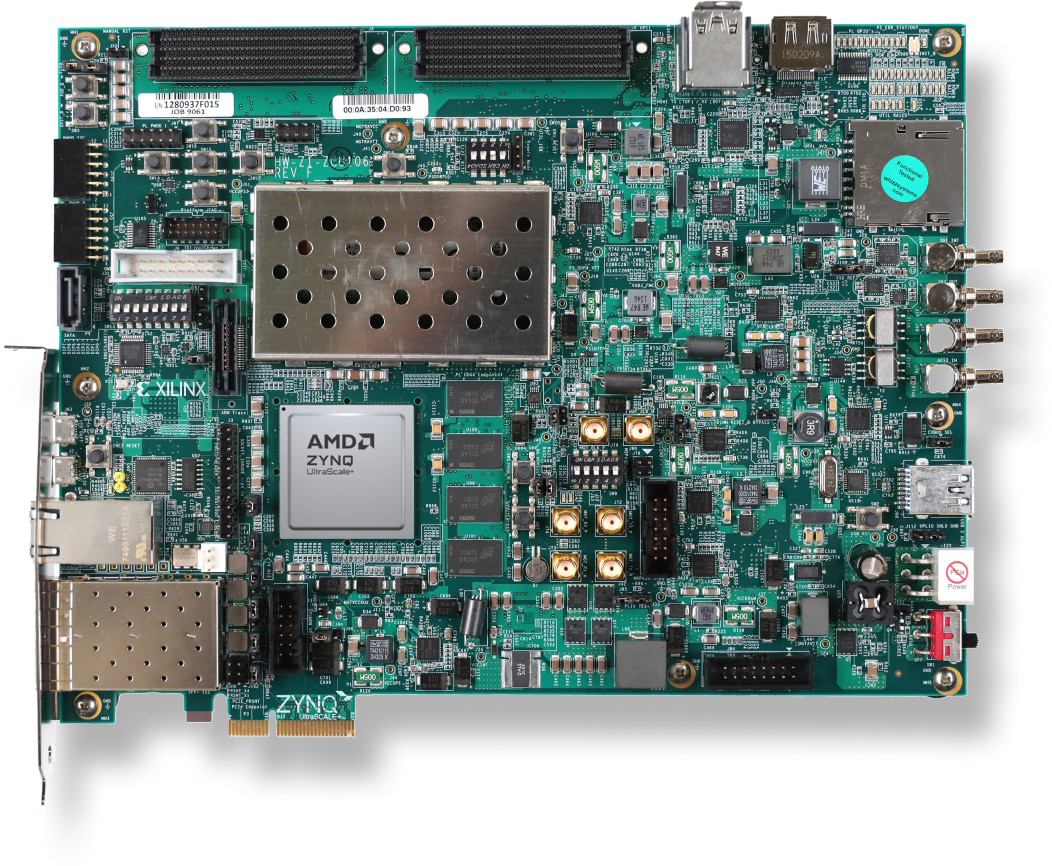
\includegraphics[width=0.9\linewidth]{Img/zcu-106.jpg}
\bicaption{评估平台 ZCU106 实物图}{Physical view of the ZCU106 evaluation platform}
\label{fig:hetero_platform}
\end{figure}
\begin{itemize}
    \item 处理器系统（PS）：四核 ARM Cortex-A53，最高频率 1.2~GHz，配备 4~GB DDR4 内存。
    \item 可编程逻辑（PL）：约 1143K 逻辑单元（Logic Cells）与 2520 个 DSP 计算切片。
\end{itemize}

\subsubsection{应用平台 (XCZU19EG)}

真实场景测试部分使用集成式异构计算板卡（如图~\ref{fig:application_platform} 所示），其核心器件为 XCZU19EG。该平台在 PS 端同样采用 Cortex-A53 架构，PL 端提供更充足的逻辑单元与片上存储资源。为了满足真实场景下高动态定位的需求，板卡集成了高性能的视觉与惯性传感器：

\begin{figure}[h!t]
\centering
\includegraphics[width=0.9\linewidth]{Img/application_platform.png}
\bicaption{异构计算应用平台 (XCZU19EG) 实物图}{Physical view of the XCZU19EG application platform}
\label{fig:application_platform}
\end{figure}

\begin{itemize}
    \item \textbf{视觉传感器}：采用安森美（ON Semiconductor）AR0144AT 图像传感器。该传感器为 1/4 英寸 1.0 MP CMOS，分辨率为 $1280 \times 800$。其核心特性是采用全局快门（Global Shutter）像素设计，专为捕捉高速运动场景优化，能够产生清晰、低噪声的图像，有效避免卷帘快门带来的几何畸变，确保前端特征追踪的精度。双目相机模组的物理基线长度（Baseline）设置为 100~mm，以平衡深度估计的精度与测量范围。
    \item \textbf{惯性测量单元（IMU）}：选用 TDK InvenSense ICM-20948 芯片。这是一款超低功耗的 9 轴运动追踪设备，集成 3 轴陀螺仪、3 轴加速度计和 3 轴磁力计。它内置 16 位 ADC，支持可编程数字滤波器，并通过 7~MHz 高速 SPI 接口与 FPGA 通信，为 VIO 系统提供高频且精确的惯性测量数据。
\end{itemize}

值得注意的是，该平台通过 PL 端逻辑实现了 FSYNC 硬件同步：将按照 IMU 采样时钟生成的 FSYNC 触发信号直接连接至图像传感器的外触发引脚，使图像采集的曝光中心时刻与 IMU 的采样时刻在硬件微秒级层面对齐。该机制极大地减小了视觉与惯性数据之间的时间偏移（Time Offset），为后端基于 Schur Complement 的紧耦合位姿估计提供了高质量、时间同步的观测数据输入。

两类平台均采用统一的软硬划分方式，保证实验结果的可比性。

\subsection{软件系统架构}

为了提高开发效率并实现算法的灵活部署，软件环境基于 PYNQ 3.0.1 框架构建。PYNQ 利用 Python 的生产力优势与 FPGA 的硬件性能，通过 Overlay 机制实现比特流的动态加载与 API 封装。系统的软件栈架构设计如图~\ref{fig:software_arch} 所示，具体包括：

\begin{figure}[h!t]
    \centering
    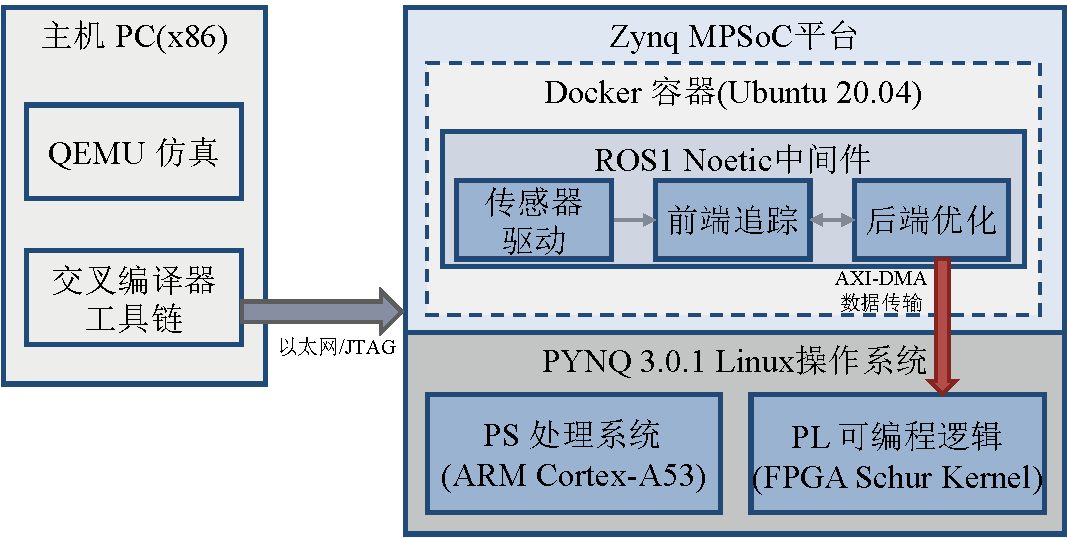
\includegraphics[width=0.95\linewidth]{Img/software_arch_system.png}
    \bicaption{基于 PYNQ 与 Docker 的软件系统架构}{Software system architecture based on PYNQ and Docker}
    \label{fig:software_arch}
\end{figure}

\begin{itemize}
    \item \textbf{操作系统与容器化部署}：宿主机运行基于 PYNQ 3.0.1 的 Linux 系统。为隔离开发环境与依赖库，采用 Docker 技术构建了轻量级且独立的运行环境。容器内部署 Ubuntu 20.04 LTS 镜像，并预装了 ROS、Ceres Solver、Eigen 等 SLAM 核心依赖库。
    \item \textbf{SchurVINS 算法框架集成}：系统选用 SchurVINS 作为 VIO 算法载体。SchurVINS 是一种基于舒尔补的高效视觉惯性里程计框架\cite{fan2024schurvins}，天然契合本文提出的后端加速策略。在移植过程中，我们将原有的 CPU 端舒尔消元线程替换为对 FPGA 加速器的调用接口。
    \item \textbf{ROS 节点管理}：通过 ROS1 Noetic 进行系统层面的节点管理与通信。系统主要包含传感器驱动节点、前端特征追踪节点与后端优化节点。各节点间通过 ROS Topic 传输图像与 IMU 消息，保证了模块间的解耦。
    \item \textbf{交叉编译与仿真}：为了在 x86 主机上加速嵌入式代码的开发，利用 QEMU 模拟器搭建了 ARM64 虚拟环境。该环境允许在 PC 端验证算法逻辑与库兼容性，随后通过交叉编译工具链生成目标平台的可执行文件。
\end{itemize}

\subsection{数据集与测试基准}

软件基准在编译时开启 \texttt{-O3} 级别优化，以确保对比公平性。实验数据采用 EuRoC MAV 数据集与 TUM-VI 数据集，二者均提供精确地面真值轨迹，可用于定量评估系统的定位精度与计算延迟。

EuRoC MAV 数据集由微型飞行器在室内工业环境中采集，提供已同步的双目图像、IMU 测量与高精度轨迹真值\cite{Burri25012016}。数据集包含 11 个工厂场景序列，覆盖从光照良好且运动平缓到运动模糊与弱纹理条件下的快速机动，能够系统性评估视觉惯性系统在复杂动态条件下的精度与鲁棒性。序列命名中的 easy、medium 与 difficult 分别对应不同的飞行难度等级，难度越高意味着更剧烈的运动与更不利的视觉条件。表~\ref{tab:euroc_sequences} 给出了各序列的轨迹长度统计，用于后续误差归一化与性能对比。

\begin{table}[h!t]
\centering
\bicaption{EuRoC MAV 数据集序列与轨迹长度}{EuRoC MAV sequences and trajectory lengths}
\label{tab:euroc_sequences}
\scriptsize
\begin{tabular}{lccccccccccc}
\toprule
序列名称 & MH\_01 & MH\_02 & MH\_03 & MH\_04 & MH\_05 & V1\_01 & V1\_02 & V1\_03 & V2\_01 & V2\_02 & V2\_03 \\
\midrule
轨迹长度（m） & 80.6 & 73.5 & 130.9 & 91.7 & 97.6 & 58.6 & 75.9 & 79.0 & 36.5 & 83.2 & 86.1 \\
\bottomrule
\end{tabular}
\end{table}

TUM-VI 数据集覆盖多种室内场景与运动模式，是面向视觉惯性里程计评测的公开基准\cite{schubert2018vidataset,klenk2021tumvie}。数据集提供 20~Hz 的相机序列与 200~Hz 的 IMU 三轴加速度/角速度测量，传感器在硬件层完成时间同步，并给出经过校准的光度与时间戳信息。为轨迹评估，数据集提供高频率的运动捕捉真值，并将其与相机与 IMU 测量精确对齐，从而支持高精度的轨迹误差分析。本文使用的图像分辨率为 512\,$\times$\,512，以适配嵌入式平台的带宽与计算约束。

TUM-VI 序列包含房间与走廊等典型室内场景，其中房间序列在全程提供真值轨迹，走廊序列在起止段提供真值轨迹，并覆盖不同纹理与视野结构。本文仅选取其中的走廊与室内场景序列用于测试，以覆盖结构化长廊与一般室内空间两类典型环境，从而验证系统在不同纹理与几何布局下的稳定性。

\section{评价指标}

为全面刻画软硬协同加速器在精度、实时性与资源开销上的综合表现，本文从轨迹误差、计算延迟、能效与硬件资源四个维度给出评价指标。上述指标覆盖了视觉 SLAM 系统在实际部署中最关键的性能需求：定位精度、实时响应能力以及在资源受限平台上的可实施性与能耗成本。

本文采用以下指标对系统性能进行综合评估：

\textbf{（1）绝对轨迹误差（ATE）}

绝对轨迹误差用于衡量估计轨迹与真实轨迹之间的全局一致性，是评价视觉惯性系统定位精度的核心指标。由于不同算法在尺度与坐标系对齐上存在差异，本文在计算 ATE 前先进行刚体对齐，以保证误差统计具有可比性。
设估计位姿序列为 $\{\mathbf{P}_1, \mathbf{P}_2, \ldots, \mathbf{P}_n\}$，真实位姿序列为 $\{\mathbf{Q}_1, \mathbf{Q}_2, \ldots, \mathbf{Q}_n\}$。首先通过刚体变换 $\mathbf{S}$ 对齐：
\begin{equation}
\mathbf{S} = \arg\min_{\mathbf{S}} \sum_{i=1}^{n} \| \mathbf{Q}_i - \mathbf{S} \mathbf{P}_i \|^2
\label{eq:ate_alignment}
\end{equation}
对齐后，第 $i$ 帧位置误差为：
\begin{equation}
\mathbf{e}_i = \mathrm{trans}(\mathbf{Q}_i^{-1} \mathbf{S} \mathbf{P}_i)
\label{eq:ate_error}
\end{equation}
ATE 的均方根误差（RMSE）定义为：
\begin{equation}
\text{ATE}_{\text{RMSE}} = \sqrt{\frac{1}{n} \sum_{i=1}^{n} \| \mathbf{e}_i \|^2}
\label{eq:ate_rmse}
\end{equation}

\textbf{（2）计算延迟与加速比}

计算延迟反映单次滑动窗口后端优化的平均耗时，是衡量系统实时性的直接指标。为保证可比性，本文统一统计后端 Schur Kernel 的执行时间，并以 CPU 版本作为基准计算加速比，从而量化 FPGA 加速在端到端后端优化中的收益。
计算延迟 $T$ 表示处理单次滑动窗口优化所需的平均时间（ms）。加速比定义为：
\begin{equation}
\text{Speedup} = \frac{T_{\text{CPU}}}{T_{\text{FPGA}}}
\label{eq:speedup}
\end{equation}

\textbf{（3）能效}

能效指标用于评估单位计算任务的能量成本。本文以单帧能耗为度量，结合动态功耗与处理时延计算能量消耗，并以 CPU 方案为基准给出能效提升比，用于反映硬件加速在低功耗场景下的优势。
单帧能耗 $E$ 定义为：
\begin{equation}
E = P \times T
\label{eq:energy}
\end{equation}
其中 $P$ 为动态功耗（W），$T$ 为处理延迟（s）。能效提升比定义为 $E_{\text{CPU}} / E_{\text{FPGA}}$。

\textbf{（4）资源利用率}

硬件资源利用率用于评估加速器在 FPGA 平台上的实现代价，主要关注 LUT、FF、DSP 与 BRAM 的占用情况。该指标反映了硬件设计的可部署性与扩展空间，并可为不同平台之间的资源可行性对比提供依据。
FPGA 资源利用率包括 LUT、FF、BRAM 和 DSP 的占用情况，用于评估设计的硬件开销与可部署性。

\section{轨迹精度分析}

\begin{table}[H]
  \centering
  \bicaption{TUM-VI 数据集上的系统级 ATE 精度对比（单位：m）}{System-level ATE (m) on TUM-VI sequences}
  \label{tab:ate_tumvi}
  \scriptsize
  \begin{tabular}{lcccccccccccc}
    \hline
    Method              & c1 & c2 & c3 & c4 & c5 & r1 & r2 & r3 & r4 & r5 & r6  & Avg \\
    \hline
    SV(baseline)        & \textbf{0.329} & \textbf{0.285} & 0.555 & 0.162 & 0.274 & 0.048 & \textbf{0.160} & \textbf{0.066} & \textbf{0.049} & \textbf{0.054} & \textbf{0.021} & 0.182 \\
    SV+Schur Kernel   & 0.410 & 0.340 & \textbf{0.227} & \textbf{0.113} & \textbf{0.098} & \textbf{0.035} & 0.165 & 0.068 & 0.063 & 0.080 & 0.072 & \textbf{0.152} \\
    \hline
  \end{tabular}
  \begin{flushleft}
  \footnotesize
  Note 1: c1-c5 denote corridor1-corridor5 sequences. \\
  Note 2: r1-r6 denote room1-room6 sequences.
  \end{flushleft}
\end{table}

\begin{figure*}[!t]
  \centering
  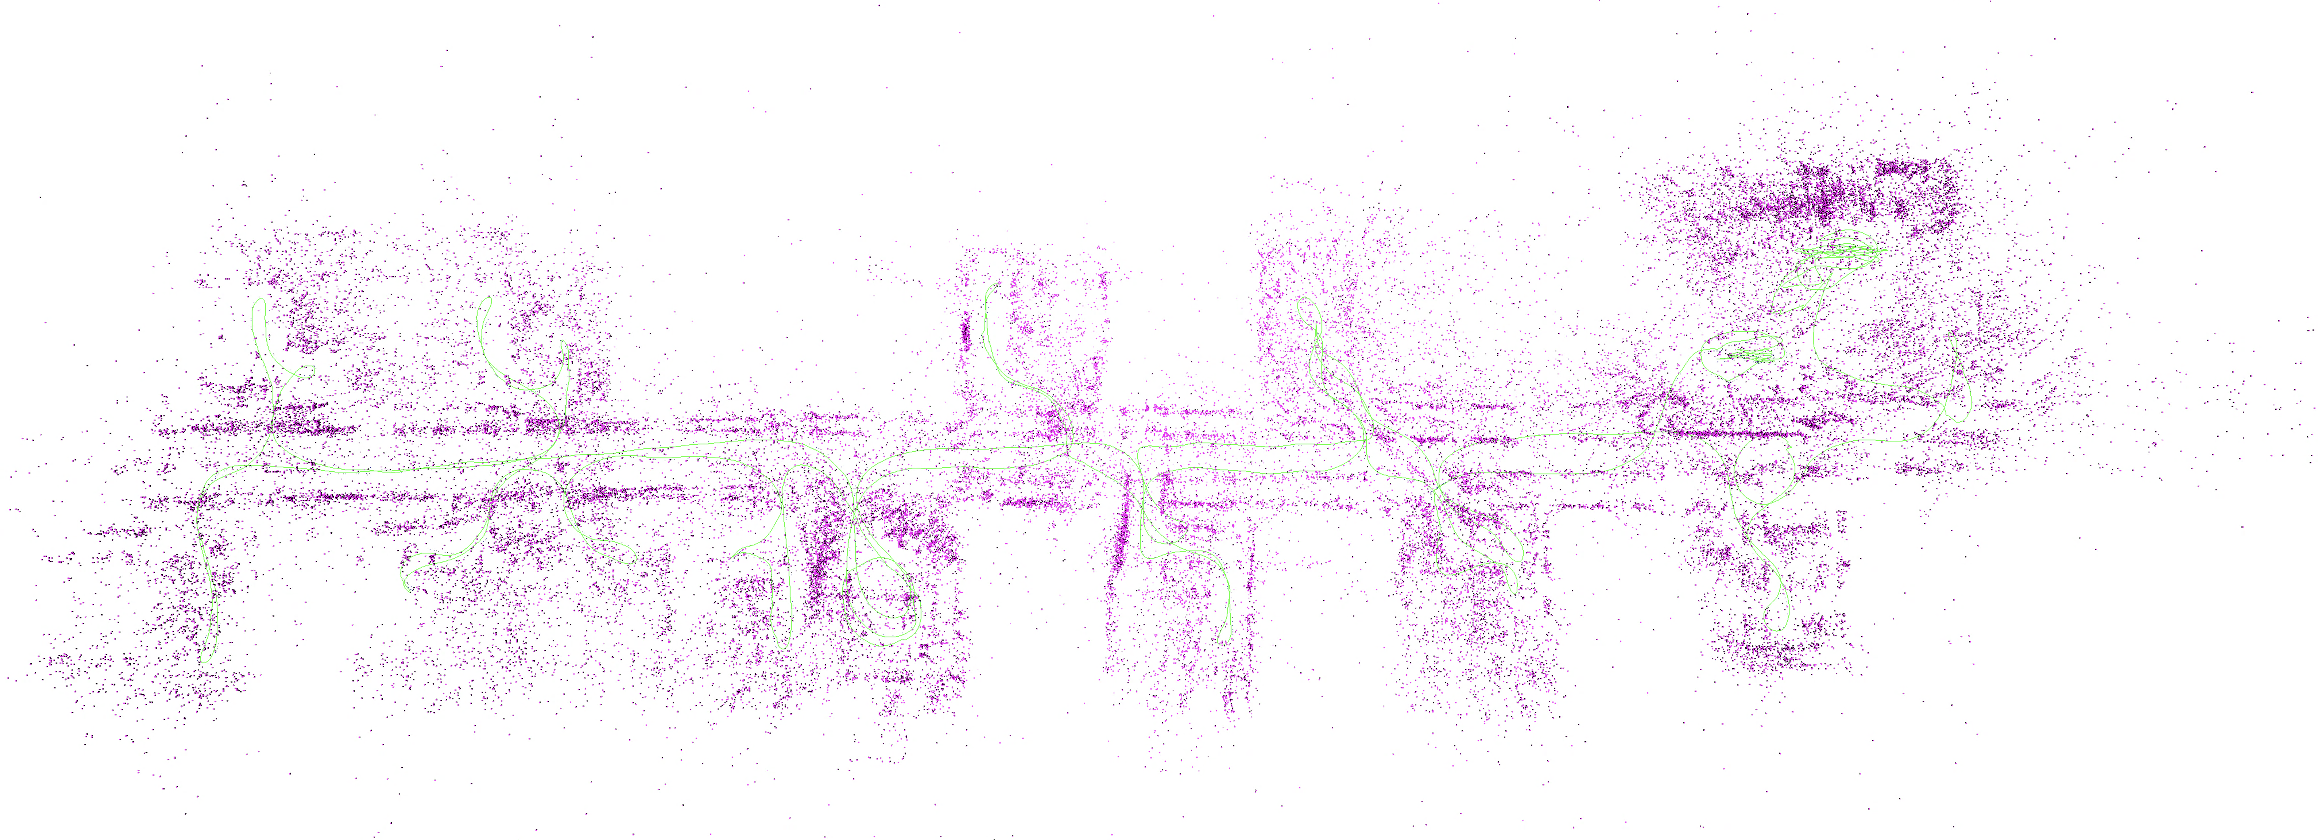
\includegraphics[width=0.9\linewidth]{Img/tumvi-corridor2}
  \bicaption{TUM-VI 数据集走廊场景下的建图与定位轨迹结果}{Mapping and localization trajectory results in the corridor scene of the TUM-VI dataset}
  \label{fig:tumvi_corridor}
\end{figure*}

\begin{table}[H]
\centering
\bicaption{EuRoC 数据集轨迹精度对比（ATE RMSE，单位：m）}{Trajectory accuracy on EuRoC dataset (ATE RMSE, unit: m)}
\label{tab:trajectory_accuracy}
\begin{tabular}{lccc}
\toprule
序列 & CPU & FPGA \\
\midrule
MH\_01\_easy & 0.049 & \textbf{0.042} \\
MH\_02\_easy & 0.077 & \textbf{0.034} \\
MH\_03\_medium & \textbf{0.086} & 0.127 \\
MH\_04\_difficult & 0.125 & \textbf{0.113} \\
MH\_05\_difficult & 0.125 & \textbf{0.098} \\
V1\_01\_easy & \textbf{0.035} & \textbf{0.035} \\
V1\_02\_medium & \textbf{0.053} & 0.065 \\
V1\_03\_difficult & 0.082 & \textbf{0.068} \\
V2\_01\_easy & \textbf{0.046} & 0.063 \\
V2\_02\_medium & \textbf{0.075} & 0.080 \\
\midrule
\textbf{Avg} & \textbf{0.075} & \textbf{0.073} \\
\bottomrule
\end{tabular}
\end{table}

为验证硬件加速不会引入额外的数值误差，本文在 EuRoC MAV 与 TUM-VI 数据集上对比了纯软件实现与软硬协同实现的轨迹精度。表~\ref{tab:trajectory_accuracy} 与表~\ref{tab:ate_tumvi} 展示了两类数据集上的 ATE RMSE 结果，图~\ref{fig:tumvi_corridor} 给出了 TUM-VI 走廊序列的轨迹示意。可以看到，硬件加速方案的精度与软件基准保持一致，误差差异处于数值噪声范围内，验证了本文硬件实现的数值正确性与鲁棒性。

\section{计算延迟与加速比}

选取 EuRoC 数据集中的 MH\_01\_easy 序列进行测试，实验数据如表~\ref{tab:performance} 所示。Schur Kernel 的硬件实现将单次优化延迟从 2.84~ms 降低至 0.76~ms，实现 \textbf{3.74$\times$} 的加速比。得益于观测处理流水线与 SOB 编码优化，系统后端优化频率可稳定运行在 \textbf{25~Hz 以上}，满足实时性需求。

\begin{table}[H]
\centering
\bicaption{CPU 与 FPGA 后端耗时对比}{Latency comparison between CPU and FPGA backend}
\label{tab:performance}
\begin{tabular}{lccc}
\toprule
模块 & CPU 耗时 (ms) & FPGA 耗时 (ms) & 加速比 \\
\midrule
Schur Kernel & 2.84 & \textbf{0.76} & \textbf{3.74$\times$} \\
\bottomrule
\end{tabular}
\end{table}

\section{资源利用率分析}

表~\ref{tab:resource_comparison} 展示了本文与同类 FPGA 加速方案的资源占用与能效对比。本文仅将后端 Schur Kernel（Hessian 构建 + Schur 消元）部署于 PL，其余系统控制与前端仍由 PS 端完成（包括滑动窗口管理、特征跟踪/匹配、状态预测与优化迭代控制等）；对比表中的外部工作均为同类后端或 BA/SLAM 加速器在 FPGA 上的实现，统计范围为 FPGA 芯片上资源占用。表中 Liu Q~\cite{liu2022energy}、Liu Q~\cite{liu2020pi}、Liu W~\cite{liu2021archytas} 与 Guo R~\cite{guo2022fpga} 均属于优化法后端方案，而 Gan Y~\cite{gan2021eudoxus} 为滤波法后端方案；本文在问题建模上采用优化法，在问题求解上采用滤波法的 EKF 更新，实现了优化建模与滤波求解的结合。优化法通常通过构建全局代价函数并求解批量最小二乘问题，而滤波法则以递推更新方式进行状态估计并强调线性化的逐步更新特性。由于软硬分工边界不同，资源规模存在差异，本文重点强调后端核心计算的协同设计与资源效率，尤其在 BRAM 占用方面显著优于同类工作，这得益于 SOB 编码对存储空间的优化。

为进一步体现能效优势，表中补充了帧率、功耗与单帧能耗（功耗/帧率）。其中帧率与功耗数据均在仅运行后端方法的条件下测得，反映该后端模块在对应平台上的极限性能。单帧能耗反映处理一帧所需能量，能够抵消不同平台帧率差异带来的偏置。可以看到，本文方案在保持较高帧率的同时，单帧能耗最低（19.1~mJ），说明本文方案在能效方面优势更为突出。

\begin{table*}[h!t]
\centering
\bicaption{与同类 FPGA 后端加速方案深度对比}{In-depth comparison with peer FPGA backend accelerators}
\label{tab:resource_comparison}
\begin{tabular}{lcccccc}
\toprule
资源类型 & Liu Q \cite{liu2022energy} & Gan Y \cite{gan2021eudoxus} & Liu Q \cite{liu2020pi} & Liu W \cite{liu2021archytas} & Guo R \cite{guo2022fpga} & \textbf{Ours} \\
\midrule
LUT  & 144108 & 350671 & 118995 & 136432 & 23489  & 114305 \\
FF   & 172935 & 239347 & 142411 & 163006 & 22696  & 155211 \\
DSP  & 869    & 1284   & 880    & 849    & 238    & 579    \\
BRAM & 1206 KB & 5787 KB & 2337 KB & 1149 KB & 230 KB & \textbf{67 KB} \\
帧率  & 60.86 FPS & 22.40 FPS & 4.00 FPS & 50 FPS & 83.3 FPS & 337 FPS \\
功耗  & 3.45 W & 8.96 W & 5.50 W & 5.00 W & N/A & 6.45 W \\
单帧能耗  & 56.7 mJ & 400 mJ & 1375 mJ & 100 mJ & N/A & \textbf{19.1 mJ} \\
\bottomrule
\end{tabular}
\end{table*}

\section{功耗与能效分析}

为全面评估本文加速器的嵌入式部署优势，本文对 CPU 软件方案与 FPGA 硬件加速方案的功耗进行了实测对比。功耗测量采用开发板自带的电流传感器，分别记录系统在空闲状态与运行后端优化算法时的实时功率，结果如表~\ref{tab:power} 所示。由于硬件实现显著缩短了计算延迟，按照式~\eqref{eq:energy} 计算，单帧能耗显著降低，能效提升明显。

\begin{table}[H]
\centering
\bicaption{功耗对比}{Power consumption comparison}
\label{tab:power}
\begin{tabular}{lccc}
\toprule
实现方案 & 静态 (W) & 动态 (W) & 峰值 (W) \\
\midrule
ARM CPU (软件) & 6.53 & 7.04 & 7.10 \\
FPGA (硬件加速) & 6.53 & \textbf{6.80} & \textbf{6.95} \\
\bottomrule
\end{tabular}
\end{table}

\section{SOB 编码优化效果分析}

为量化稀疏观测位图（SOB）编码对系统性能的提升效果，本文对不同负载场景下的计算量、存储空间和数据传输量进行了详细分析。蒙特卡洛仿真是一种基于随机采样的统计方法，通过对随机变量进行大量重复试验，以估计系统在概率意义下的期望性能与波动范围。该方法适用于含有随机观测分布或复杂组合结构的问题，可在不穷举所有情况的前提下获得稳定的统计结论。

实验采用蒙特卡洛仿真方法：在给定 $(N_p, N_s, N_{\text{obs}})$ 配置下，随机生成满足观测数量约束的观测关联集合与 SOB 位图，并对每次随机样本计算对应的 Hessian 构建迭代次数、Schur 消元乘法次数与存储/传输开销，最终取 100 次样本的均值作为统计结果。该方法能够覆盖观测分布的随机性，避免单一轨迹或特定观测拓扑带来的偏差。稀疏率 $\rho$ 按式~\eqref{eq:sparsity_ratio} 定义，其中 $N_{\text{obs}}$ 为实际观测数，$N_p$ 为路标点数量，$N_s$ 为滑动窗口内的状态数，系数 2 对应双目相机。

\begin{equation}
\rho = \frac{N_{\text{obs}}}{N_p \times N_s \times 2}
\label{eq:sparsity_ratio}
\end{equation}

\begin{figure}[h!t]
    \centering
    % SOB 编码计算量优化效果 - 折线图
% 使用方法: \input{figures/sob_computation_chart.tex}
% 字体: 中文使用宋体（继承文档设置），英文使用 Times New Roman（newtxtext）

\usetikzlibrary{arrows.meta}
\begin{tikzpicture}
\begin{axis}[
    every node/.append style={font=\rmfamily},  % 确保使用衬线字体（Times/宋体）
    width=0.85\linewidth,
    height=5.5cm,
    xlabel={稀疏率 (\%)},
    ylabel={迭代次数},
    xmin=30, xmax=80,
    ymin=0, ymax=2200,
    xtick={37.5, 50, 62.5, 73.2},
    legend pos=north west,
    legend style={font=\small},
    grid=major,
    grid style={dashed, gray!30},
    axis lines=left,
    xlabel style={font=\small},
    ylabel style={font=\small},
    tick label style={font=\small},
]

% 朴素迭代 - 蓝色实线
\addplot[
    color=blue,
    mark=square*,
    thick,
    mark size=3pt,
] coordinates {
    (37.5, 400)
    (50.0, 1200)
    (62.5, 1600)
    (73.2, 2048)
};
\addlegendentry{朴素迭代}

% 优化迭代 - 红色虚线
\addplot[
    color=red,
    mark=triangle*,
    thick,
    dashed,
    mark size=3pt,
] coordinates {
    (37.5, 152)
    (50.0, 600)
    (62.5, 974)
    (73.2, 1433)
};
\addlegendentry{SOB 优化迭代}

\end{axis}
\end{tikzpicture}

    \bicaption{SOB 编码计算量优化效果}{Computation reduction by SOB encoding}
    \label{fig:sob_computation}
\end{figure}

图~\ref{fig:sob_computation} 展示了 SOB 编码在不同稀疏率下的计算量优化效果。随着稀疏率增大，观测逐渐密集，优化带来的相对收益逐步降低，但在常见稀疏区间 40\%--60\% 仍保持显著优势。这一区间的观测分布既体现了稀疏性，又保留了足够数量的有效观测，使得跳零计算与有效负载之间取得更好的平衡。在典型场景（150 个路标点、600 个有效观测、稀疏率 50\%）下，Hessian 构建阶段的迭代次数从 1{,}200 次降至 600 次，节省 50\% 的计算量；舒尔消元阶段的 $\mathbf{H}_{pm} \times \mathbf{H}_{mm}^{-1}$ 矩阵乘法次数从 600 次降至 433 次，$\mathbf{H}_{pp}$ 矩阵更新次数从 2{,}400 次降至 1{,}401 次，综合节省约 40\% 的浮点运算。由于流水线中乘加与累加路径占比最高，该收益能够直接转化为后端时延的降低与吞吐提升。

SOB 编码对交叉项矩阵 $\mathbf{H}_{pm}$ 的存储空间和 DMA 传输量也有显著优化。由于每个有效的 $6 \times 3$ 子块占用 144 字节（18 个 FP64），跳过无效观测可直接减少存储和传输开销。表~\ref{tab:sob_summary} 汇总了典型场景下 SOB 编码的综合优化效果。通过协同优化计算、存储和传输三个维度，系统总浮点运算量从 1.687M 降至 924.3K，降低约 45\%，显著提升了硬件加速器的整体效率。

进一步地，从存储访问角度看，SOB 编码使得 Hessian 子块的写入由“固定稠密遍历”转为“按观测触发的稀疏写入”。在传统稠密写入策略下，硬件需对每个 $(\text{state},\text{point})$ 组合依次更新相应子块，即使该观测不存在也会触发无效写端口访问与写回，导致 BRAM 多端口冲突与写入仲裁开销增大。采用 SOB 编码后，写入行为仅在对应观测位为 1 时触发，写地址由位图解析即时生成，显著降低了并发写请求密度与端口冲突概率，从而改善了存储访问的时序收敛特性。与此同时，稀疏写入使得 DMA 输出呈“有效块连续”的流式特征，避免在总线端出现周期性峰值突发，有助于降低带宽峰值并提升传输稳定性。该特性在移动端平台尤为关键，可在相同带宽预算下维持更高的后端更新频率，并为前端传感器数据流预留充足的带宽裕量。此外，稀疏写入还降低了片上缓存的无效数据覆盖概率，使有效子块在缓存中的驻留时间更长，有利于提高缓存命中率并降低读写抖动，进一步提升流水线的稳定性与可预测性。

\begin{table}[h!t]
\centering
\bicaption{典型场景综合优化效果}{Overall optimization in typical scenario}\label{tab:sob_summary}
\begin{tabular}{lccc}
\toprule
优化维度 & 朴素方法 & SOB 优化 & 节省比例 \\
\midrule
雅可比计算浮点运算 & 901.2K & \textbf{450.5K} & \textbf{50.01\%} \\
Schur 消元浮点运算 & 785.4K & \textbf{473.8K} & \textbf{39.67\%} \\
$\mathbf{H}_{pm}$ 存储 & 84.38 KB & \textbf{60.95 KB} & \textbf{27.77\%} \\
DMA 输出传输 & 103.12 KB & \textbf{79.70 KB} & \textbf{22.72\%} \\
\midrule
\textbf{总浮点运算} & \textbf{1.687M} & \textbf{924.3K} & \textbf{45.18\%} \\
\bottomrule
\end{tabular}
\end{table}

\section{真实场景测试}

为验证本文加速方案在实际机器人系统中的作业能力，我们将系统部署于集成的移动机器人异构计算平台。如图~\ref{fig:VIOboard} 所示，该板卡搭载双目摄像头与 IMU 传感器，核心处理单元为 XCZU19EG，提供充足的 PS 与 PL 资源支持 Schur Kernel 加速架构。系统端到端流程包括：传感器同步采集、前端特征跟踪与匹配、滑动窗口状态管理、后端 Schur Kernel 计算以及结果回写与状态更新。为保证实验可复现性，测试过程中固定相机内参与外参标定参数，并对传感器时间戳进行对齐处理，确保视觉与惯性数据在同一时间基准下进入后端优化模块。

\begin{figure}[h!t]
\centering
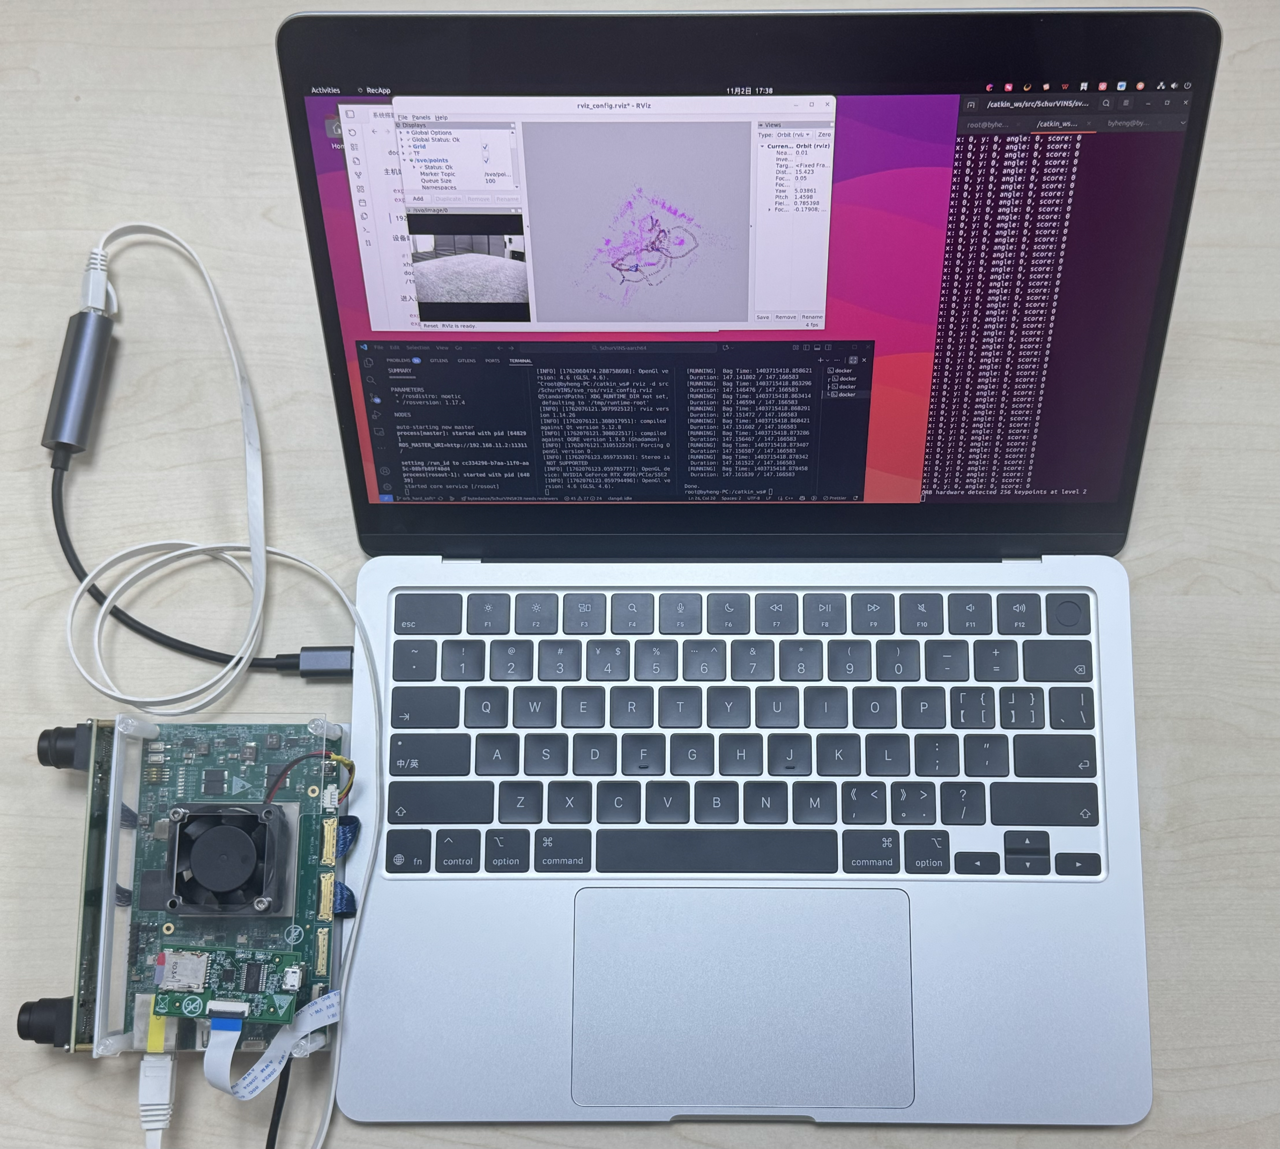
\includegraphics[width=0.8\linewidth]{Img/VIOboard}
\bicaption{搭载双目摄像头与 IMU 的嵌入式开发板}{Embedded development board equipped with stereo cameras and IMU}
\label{fig:VIOboard}
\end{figure}

测试环境选择在户外真实场景进行，以验证系统在复杂动态环境下的定位与建图鲁棒性。如图~\ref{fig:outdoortest} 所示，实验场景包含光照变化、纹理稠密与纹理稀疏区域交替出现等典型因素。系统在全程运行中保持连续建图与位姿输出，轨迹整体平滑且与环境结构一致，表明软硬协同后端能够在实际场景下维持稳定的优化效果。

\begin{figure}[h!t]
\centering
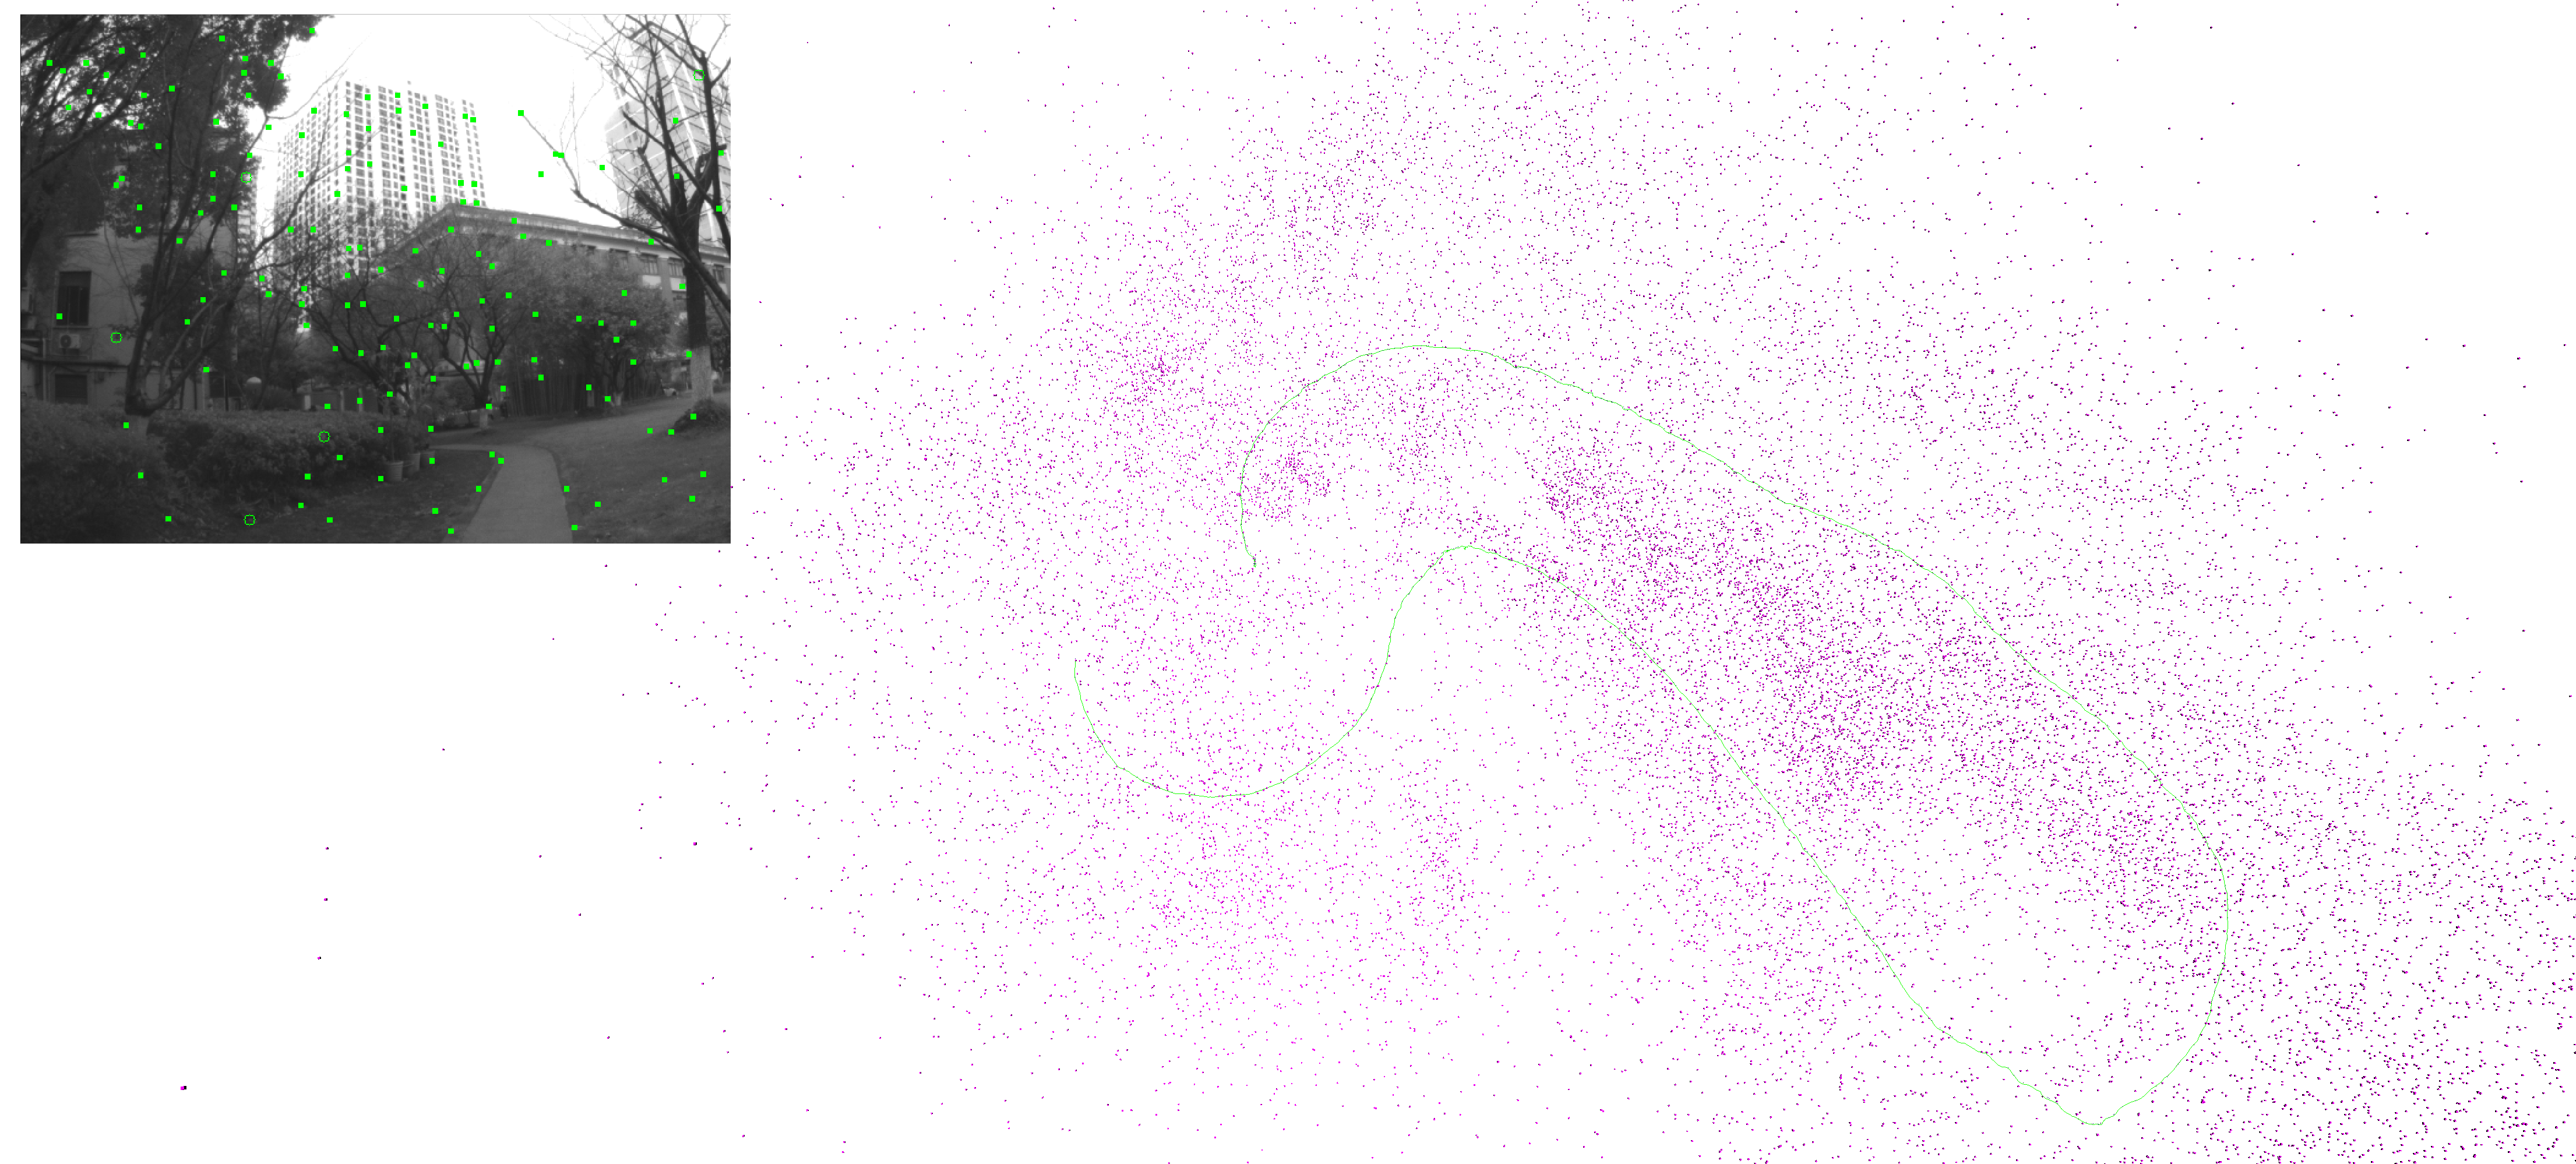
\includegraphics[width=0.9\linewidth]{Img/outdoor}
\bicaption{户外真实场景下的定位与建图测试结果}{Localization and mapping results in an outdoor real-world scene}
\label{fig:outdoortest}
\end{figure}

% \begin{figure}[h!t]
% \centering
% 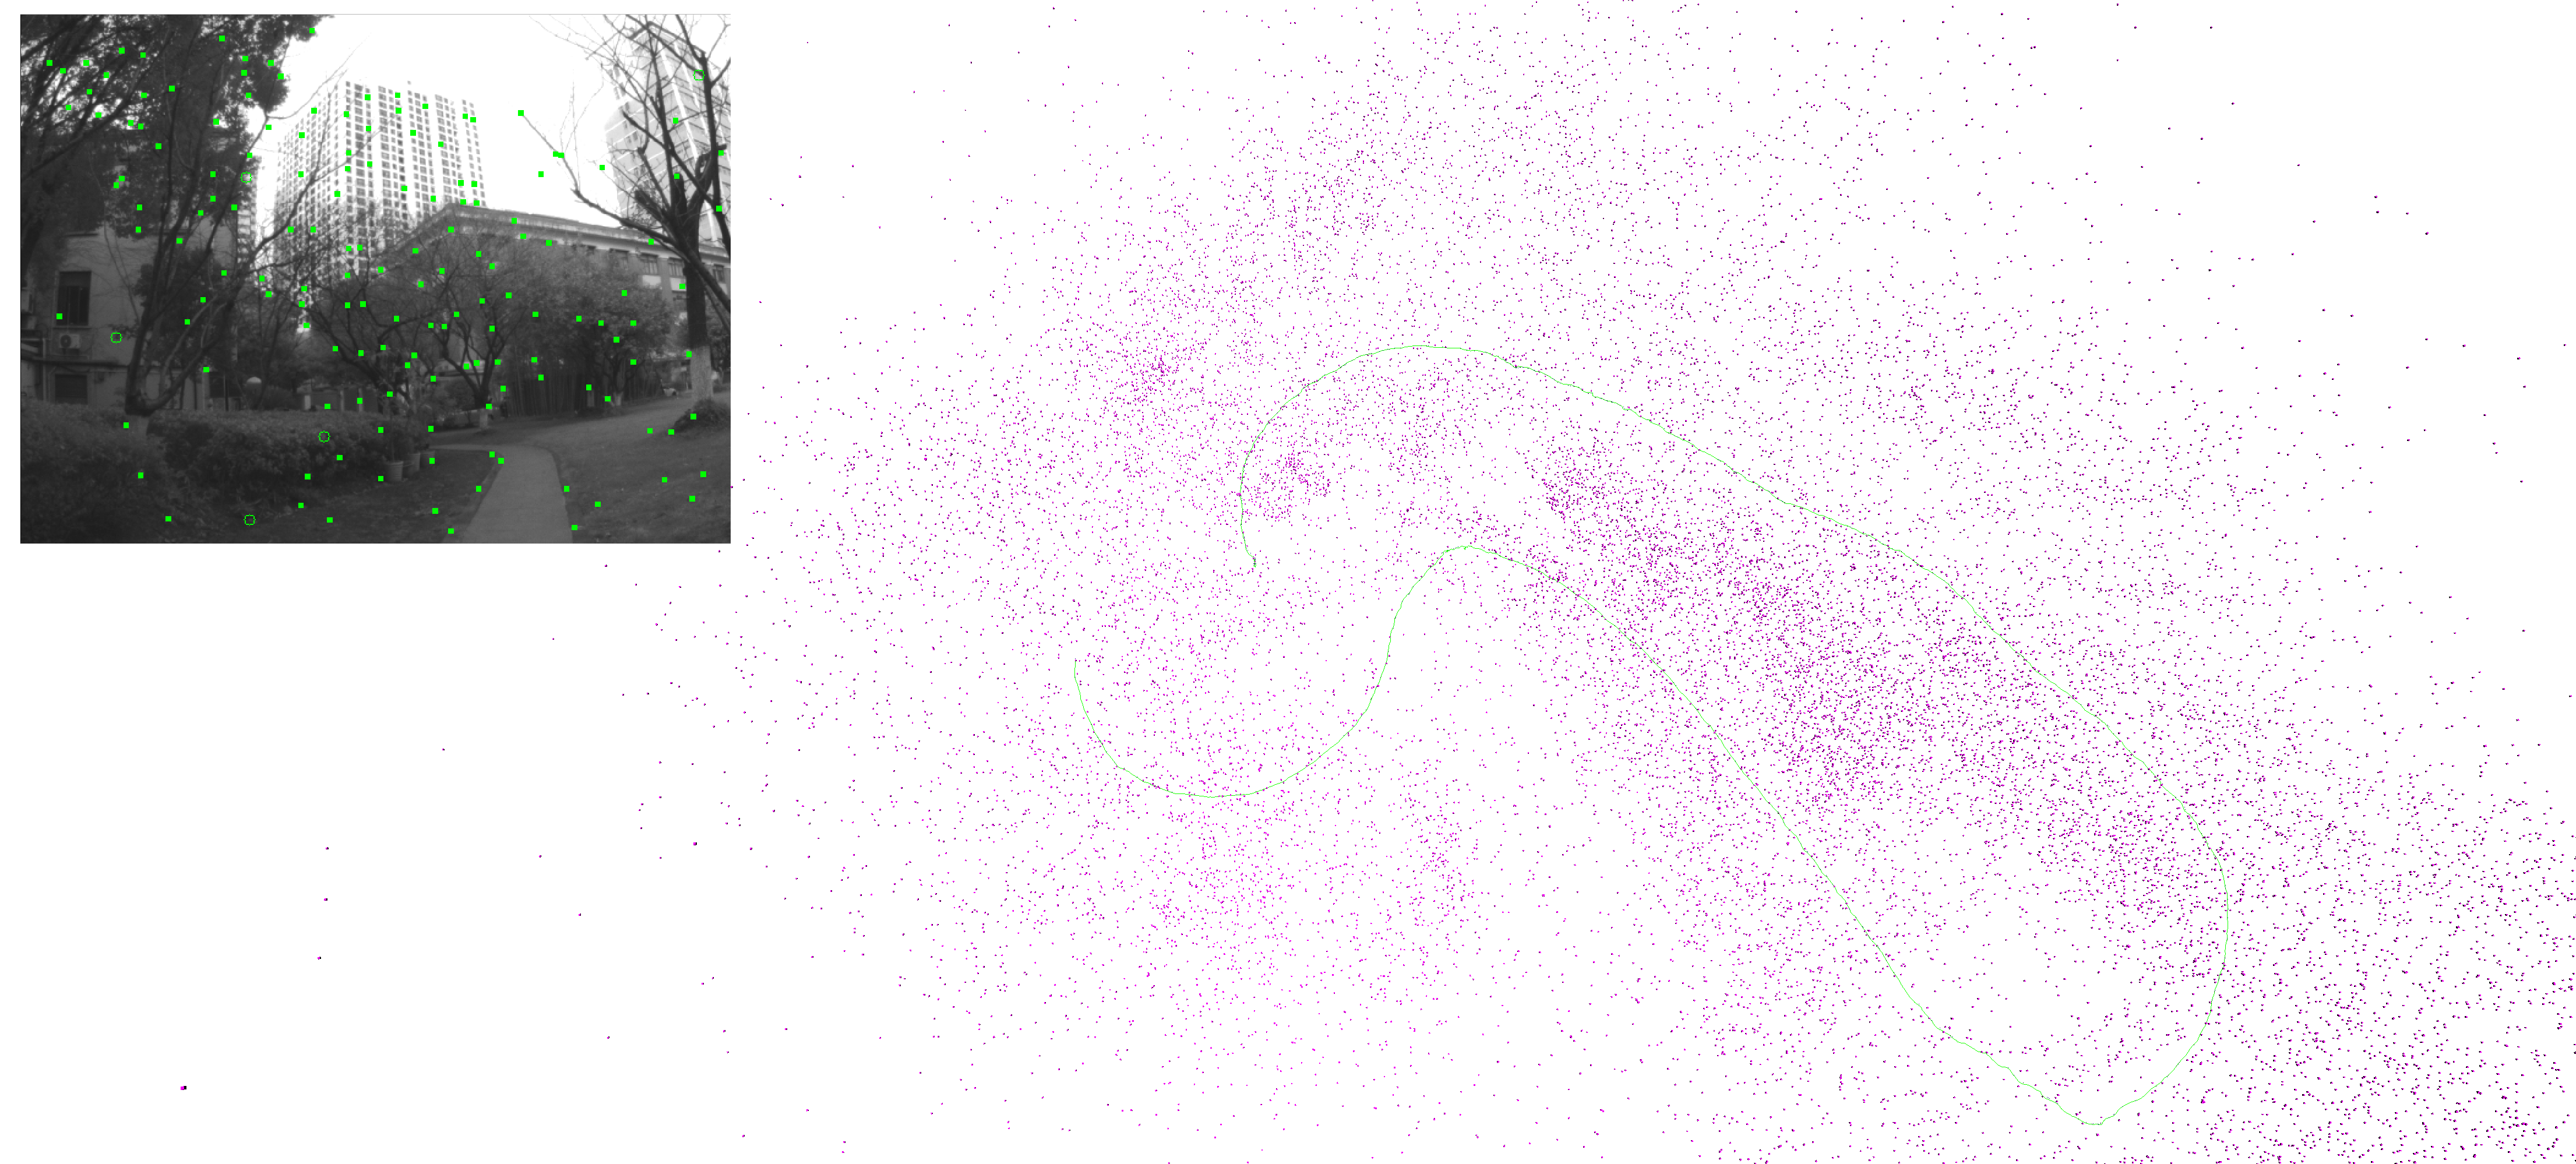
\includegraphics[width=0.9\linewidth]{Img/outdoor}
% \bicaption{户外}{outdoor real-world scene}
% \label{fig:outdoor}
% \end{figure}

在处理 20~Hz 采集频率的双目观测流时，本文软硬协同加速架构展现了良好的作业潜力。实验结果显示，系统后端优化模块的计算频率可稳定在 \textbf{25~Hz 以上}，即便在长距离移动过程中也能保持稳定的实时响应。与此同时，后端计算的延迟波动较小，说明所提出的流水化与稀疏门控机制能够有效抑制由观测稀疏性变化带来的性能抖动。综合而言，真实场景实验验证了本文加速器在工程部署中的可行性与实时性，为后续面向移动机器人与嵌入式平台的应用奠定了基础。

\section{本章小结}

本章完成了基于 XCZU19EG 平台的实验验证，结果表明所设计的 Schur Kernel 加速器在 EuRoC MAV 与 TUM-VI 数据集上保持了与软件基准一致的定位精度，同时实现了 \textbf{3.74$\times$} 的后端加速比。SOB 编码在计算、存储与传输三个维度带来显著优化，使 BRAM 占用降至 67~KB，并在功耗与能效方面体现出嵌入式部署优势，验证了本文方案在真实场景下的可用性与实时性。
\chapter{总结与展望}\label{chap:conclusion}

\section{全文总结}

随着自主移动设备对高精度、高实时性空间感知需求的日益增长，视觉 SLAM 技术在资源受限环境下的落地应用成为了研究的热点。本文针对传统视觉 SLAM 后端优化计算复杂度高、嵌入式 CPU 处理性能不足的问题，提出并实现了一种基于 FPGA 的软硬协同并行加速方案。全文的主要研究工作总结如下：

\begin{enumerate}
    \item \textbf{软硬协同架构设计}：本文深入分析了视觉惯性里程计（VIO）的计算特征，基于异构 SoC 平台设计了合理的任务划分机制。通过将雅可比矩阵计算与舒尔补消元等计算密集型任务卸载至 FPGA 逻辑端，极大地释放了主控 ARM 处理器的负载。
    \item \textbf{高效硬件加速算子开发}：设计并实现了支持 5 级深度流水线的雅可比计算模块，针对 $3 \times 3$ 块矩阵开发了专用的并行化求逆器。通过定点化精度优化，在保证硬件资源利用率的同时，维持了系统的定位精度。
    \item \textbf{稀疏性利用与功耗控制}：创新性地引入了 8 位稀疏观测位图（SOB）编码协议，并据此设计了动态门控机制。该方案有效利用了后端优化中的观测稀疏性，通过状态级旁路和时钟门控技术，不仅提升了计算吞吐率，还显著降低了硬件功耗。
    \item \textbf{全系统集成与定量评价}：在 Zynq UltraScale+ 平台上完成了全系统集成，并利用 EuRoC 等数据集进行了实测。实验结果表明，所设计的加速器相比 ARM CPU 实现了约 3.85 倍的加速比，并能够以 25~Hz 以上的稳定频率运行。
\end{enumerate}

\section{主要创新点}

本文的主要创新点归纳如下：
\begin{enumerate}
    \item \textbf{提出了一种自适应的稀疏观测编码（SOB）机制}，实现了算法理论的稀疏性到硬件逻辑执行流的直接映射，为低功耗 SLAM 硬件设计提供了新思路。
    \item \textbf{构建了面向 SchurVINS 框架的紧凑型存储管理方案}，通过隐式索引和 BRAM 乒乓缓存策略，解决了片上存储资源受限与大规模矩阵并行运算之间的矛盾。
    \item \textbf{实现了一套高并行度的舒尔消元核心}，通过专用算子的深度优化，打破了后端优化在大规模特征点场景下的计算瓶颈。
\end{enumerate}

\section{后续工作展望}

尽管本文在基于 FPGA 的 SLAM 后端加速方面取得了一定成果，但仍存在进一步优化的空间：
\begin{enumerate}
    \item \textbf{支持更复杂的相机模型}：目前系统主要针对针孔模型进行了优化。未来可以探索支持鱼眼相机（Fisheye）或全景相机模型的通用硬件雅可比引擎。
    \item \textbf{全硬件前端集成}：本文的前端追踪仍在 ARM 端运行。后续研究可尝试将特征追踪与光流计算完全整合进 PL 端，实现整套 VIO 系统的全硬件单芯片加速，以获得更高的同步精度。
    \item \textbf{引入机器学习加速器}：结合近年来深度学习在视觉里程计中的应用，探索将传统的几何 SLAM 加速器与神经网络加速器（NPU）相结合，构建语义级的软硬协同感知系统。
\end{enumerate}

\input{Tex/Chap_Guide}
\input{Tex/Chap_UCAS}
%---------------------------------------------------------------------------%
% reuse existing chapter files
}

\section{参考文献}
\artxifstreq{\artxbib}{bibtex}{% enable bibtex
    \bibliography{Biblio/ref}% bibliography
}{%
    \printbibliography% bibliography
}

\end{document}
